\documentclass{thesis}

\usepackage{lipsum}
\usepackage[utf8]{inputenc}
\usepackage[ngerman,english]{babel}
\usepackage{amsmath}
\usepackage{amsthm}
\usepackage{adjustbox}
\usepackage{pdflscape}
\usepackage[toc,page]{appendix}
\usepackage{graphicx}
\usepackage{caption}
\usepackage{lmodern}
\usepackage{float}
\usepackage{sidecap}
\usepackage{pgfplots}
\usepackage{pgfplotstable}
\usepackage{tabularcalc}
\usepackage{todonotes}
\usepackage{hyperref}
\usepackage{minted}
\usepackage{siunitx}
\usepackage{acronym}
\usepackage{subfig}
\usepackage{tabularx}
\usepackage{setspace}
\usepackage[customcolors]{hf-tikz}
\usepackage{url}
\usepackage{csquotes}
\usepackage{booktabs}
\usepackage[T1]{fontenc}
\usepackage[alldates=long]{biblatex}
\addbibresource{thesis.bib}
\graphicspath{{images/}}
\pgfplotsset{compat=1.12}

\title{Privacy implications of exposing Git meta data}
\author{Arne Beer}

\pagenumbering{roman}
\begin{document}

\begin{titlepage}
    
\includegraphics[width=6.8cm]{./pic/up-uhh-logo-u-2010-u-farbe-u-rgb.pdf}
    \begin{center}\Large
        % Universität Hamburg \par
        % Fachbereich Informatik
        \vfill
        Bachelor thesis
        \vfill

        \makeatletter
        {\Large\textsf{\textbf{\@title}}\par}
        \makeatother

        \vfill
        presented by
        \par\bigskip

        \makeatletter
        {\@author} \par
        \makeatother

        born on the 21st of December 1992 in Hadamar \par
        Matriculation number: 6489196 \par
        Department of Computer Science
        \vfill

        \makeatletter
        submitted on {\@date}
        \makeatother

        \vfill
        Supervisor: Dipl.-Inform. Christian Burkert \par
        Primary Referee: Prof.\ Dr.-Ing. Hannes Federrath \par
        Secondary Referee: Prof.\ Dr.\ Dominik Herrmann

    \end{center}
\end{titlepage}

\cleardoublepage{}

\chapter*{Abstract}

Software developers use many tools during their daily work and expose lots of data, often without being aware of doing so.
This data could be used to surveil, to spy on or to influence these developers.

Recent events as the Facebook scandal, in which the data of several million people has been exposed to a consulting company~\footnote{`Facebook scandal hits 87 million users' BBC.com, http://www.bbc.com/news/technology-43649018 (accessed, 24.04.2018)}, show how data can be abused to extract valuable knowledge and can be used for malicious purposes.

This thesis aims to give an example of how much information can be exposed by simply using the popular \ac{vcs} \emph{Git}.
Simple metadata such as UNIX timestamps and email addresses might be enough to extract sensitive information about users or organizations using Git.
This paper covers the whole process of gathering data from a vast amount of Git repositories, through to preprocessing, generating and interpreting the results of the analyses.
With this thesis, I hope to raise the awareness how dangerous it can be to expose even simple metadata and to proof that it can be used maliciously.

\clearpage

\vspace*{\fill}
\thispagestyle{empty}
\begin{quotation}
    \em
    Gotta go fast.

    \medskip
\raggedleft{}
    Senic the Herdgherd
\end{quotation}
\vspace*{\fill}


% Set table of contents depth
\setcounter{secnumdepth}{1}
\setcounter{tocdepth}{1}
{\small \tableofcontents}

\chapter*{Acronyms}
\begin{acronym}
    \acro{api}[API]{Application Programming Interface}
    \acro{cet}[CET]{Central European Time}
    \acro{cest}[CEST]{Central European Summer Time}
    \acro{cpu}[CPU]{Central Processing Unit}
    \acro{cvcs}[CVCS]{Centralized Version Control Systems}
    \acro{dbscan}[DBSCAN]{Density-Based Spatial Clustering of Applications with Noise}
    \acro{dst}[DST]{daylight saving time}
    \acroplural{dst}[DSTs]{daylight saving times}
    \acro{eu}[EU]{European Union}
    \acro{fs}[FS]{file system}
    \acro{gdpr}[GDPR]{General Data Protection Regulation}
    \acro{gb}[GB]{Gigabyte}
    \acroplural{gb}[GBs]{Gigabytes}
    \acro{http}[HTTP]{Hypertext Transfer Protocol}
    \acro{iana}[IANA]{Internet Assigned Numbers Authority}
    \acro{io}[I/O]{Input/Output}
    \acro{json}[JSON]{JavaScript Object Notification}
    \acro{mit}[MIT]{Massachusetts Institute of Technology}
    \acro{orm}[ORM]{Object-Relational Mapping}
    \acro{os}[OS]{Operating System}
    \acroplural{os}[OSs]{Operating Systems}
    \acro{sha1}[SHA-1]{Secure Hash Algorithm 1}
    \acro{ssh}[SSH]{Secure Shell}
    \acro{sql}[SQL]{Structured Query Language}
    \acro{tb}[TB]{Terrabytes}
    \acro{url}[URL]{Uniform Resource Locator}
    \acroplural{url}[URLs]{Uniform Resource Locators}
    \acro{utc}[UTC]{Coordinated Universal Time}
    \acro{vcs}[VCS]{version control system}
    \acroplural{vcs}[VCSs]{version control systems}
\end{acronym}


\chapter{Introduction}
\pagenumbering{arabic}
Git is a \ac{vcs} used by most programmers on a daily basis these days.
Its purpose is to help developers version and manage the code base of their projects.
According to the Eclipse Community Survey, about 42.9\% of professional software developers used Git in 2014 with an upward tendency~\cite{article:git-popularity}.
It is deployed in many, if not most, commercial and private projects and generally valued by its users.
On top of this, it allows collaborating with thousands of contributors on the same project whilst maintaining a clear version history.

Several million users send new commits to their Git repositories every day.
On Github alone, the currently biggest open source platform, there exist about 25 million active repositories and a total of 67 million repositories~\cite{article:github-statistics}.

Some well-known projects and organizations use Git, for example, Linux, Microsoft, Ansible, and Facebook~\cite{article:github-statistics}.
Each of those repositories contains the complete contribution history of every contributing user and every contribution contains all changes, a timestamp, a message from the author and their email address.

This raises the question how much information is hidden in this metadata of a Git repository and which attack vectors could be introduced by analyzing this information.
Could it be used to harm or manipulate a contributor or maybe even a company?

The gained knowledge could be utilized by employers to spy on their employees.
It could be used by an unknown attacker, who aims to obtain sensitive information about a company and its employees through their open-source projects.
It is also imaginable, that a private individual uses this data to monitor another person, who regularly contributes to open-source repositories.

As there have not been any papers published about this specific topic yet or at least no public paper and as Git plays such a crucial role in today's software development, I want to investigate and evaluate this potential threat.
Furthermore, I want to create a foundation for future research and provide a first example of how such attacks might look like.

\section{Motivation}
Each year more and more data is collected by employers.
A study conducted by \ac{mit} students shows, that data-driven companies, that collect data about everything in their company, are about 5\% more productive~\cite{article:management-revolution}, but this should never justify any invasion into their employees' privacy.
Privacy violation already goes as far as tracking medical records of employees, which is a service provided by the company \emph{Castlight}~\cite{article:medical-data}.
Some parties warn against surveillance of employees by the management and demand stricter handling of employee data~\cite{article:vermessung-belegschaft}

Generally, it can be said, that we need to take better care of our personal information and that people need to know in which ways they can leak information.
This thesis aims to show this on the example of the \ac{vcs} Git, which is by itself a very handy tool for code versioning of a project.
It was not developed with any malicious intent, but it might be used for such.

\section{Leading Questions and Goals}

The primary research objective of this thesis is to find out if data mining on Git metadata would be feasible.
This question is explored by looking at various data mining techniques and applying them to aggregated data from Github.

To gather data and to perform analysis on the data for the purpose of this thesis, a program called \emph{Gitalizer} is developed.
It is capable of continuously collecting data from Github in several ways.
Furthermore, three different analysis methodologies and several evaluation methods for these are implemented.

\section{Outline}
This thesis examines the process and capabilities of building a data mining software based on Git metadata.
The Introduction will explain the motivation, the approach and the goals of this thesis.
In Chapter 2 three different attack models will be constructed to determine possible attack goals.
In this context related work will be mentioned with respect to the attack goals.
Chapter 3 will explain the requirements to the data, existing solutions and the process of building an own aggregator, which collects data from Github.
Chapter 4 shows the actual approach and algorithmic implementation of three different attacks.
Chapter 5 evaluates the results of the previously presented algorithms by comparing it with real-world ground truth and conducting small surveys.
In Chapter 6 the overall results of this research will then be discussed and an outlook will be provided.


\chapter{Attacks Goals and Related Work}\label{related-work}
This chapter will show the creation of several attack models, which are used to design possible attacks and outline the requirements to the data needed for these tests.
In the same context, several related works will be mentioned in reference to the particular attacks.
Additional related work, which is not directly related to any attacks is listed in a separate section.


\section{Attack Models}\label{attack-models}
In the following, I will present three attacker models, which were used to design the attack goals in the next section.
Each attacker model represents an interest group, which might use Git metadata to surveil, spy upon, manipulate or harm a target.
A number of possible valuable information about a target, which might be obtainable by analyzing Git metadata, are stated for each model.

\begin{description}
    \item[The Employer] \hfill \\
        This attack model deals with the scenario of an employer who wants to monitor their employees.
        The attacker's motivation is to spot irregularities in working behavior and thereby unmotivated or unproductive employees.
        Information gained by this attack, such as productivity metrics of employees, compliance with working hours and sick leave, could be used to surveil employees without their consensus.

    \item[The Individual] \hfill \\
        This scenario describes a single person, who wants to harm, monitor or gain information about an open-source developer.

        A possible goal of the attacker could be to either stalk the victim, cause harm in any way or manipulate it or one of their acquaintances.
        The motivation of this attacker is mostly personal and on an emotional level.
        For this purpose, the attacker could use information about the target such as relationships to other developers, sleeping rhythm, and daily routines.

        Another nonemotional attacker motive could be a robber trying to find the perfect time window to rob a house.
        Information about the geographic location of the target at a specific time or knowledge about when the target is at work could be used for this purpose.

        A third attacker motive could be a headhunter, that tries to get information about the skills and reliability of a developer.
        Several metrics, such as productivity, sick leave tendencies, geographic location and daily routine could be used for this purpose.

    \item[The Industrial Spy]~\label{attack:industrial-spy} \hfill \\
        This attack model covers the scenario of an external person, who wants to gain as much private or malicious information about a company as possible.
        The attacker's motivation is either to harm the company, gain an advantage as a competitor or in the stock market or to sell secret information to a third party.
        This attack vector only works if the targeted company is providing their full product or at least parts of their product as open-source software.

        Valuable information for this attacker is, for instance, a list of company employees, the company employee history, the geographic location of the company's workforce and internal team structures of the company.
\end{description}


\section{Attack Goals}\label{attack-goals}
This section attends to the establishment of several attack goals, which could be pursued by an attacker.
These goals serve as a guideline for the data aggregation process, which will be covered in the next chapter.
It needs to be noted, that only a few these listed attacks will be actually performed in the scope of this thesis, but this listing also serves as an exhibition of some possible attacks for anyone that wants to further investigate this topic.

\begin{description}
    \item[Productivity of Employees]~\label{attack:employer-monitoring} \hfill \\
        An employer wants to ensure that their employees work sufficiently.
        For this approach, several values could be used to create a metric of quality and quantity of work.

        In~\cite[p.~3]{article:job-productivity} simple productivity measurements such as counting the contributed lines of code and the number of function points are evaluated.
        It is stated, that these measurements indeed provide a metric for the quantity of code, but not about the actual quantity of work and quality of the code.
        In~\cite[p.~43]{article:measuring-programming-quality} the author recommends to also consider the number of removed defects from the code.
        The authors of~\cite[p.~257]{article:software-productivity} also include code style quality measurements such as \emph{cyclomatic complexity}, \emph{coupling} and lack of cohesion of methods.

        The gained information by this attack could, for instance, be used to compare the productivity of several employees with the intent to dismiss all employees that do not perform well enough in relation to their coworkers.
        Another possible use case could be the revelation of developers with a specific skill set for headhunters.
        The data needed for this attack are the additions and deletions of all commits as well as all commit timestamps and the full patches of each commit.

    \item[Compliance of Working Hours] \hfill \\
        The aim of this attack is to allow employers to check whether an employee is productive in the given working hours.
        This might be especially useful to supervise employees, that work remotely and cannot be locally monitored.

        In~\cite{article:do-programmers-work-at-night} a survey on repositories of \emph{Mozilla} and \emph{Apache} is conducted, to detect at what time their developers work.
        For this purpose, all commit timestamps of those repositories have been collected and analyzed.
        Their survey discovers that about 66\% of conducted developers follow office hours.

        The data needed for this attack are commit timestamps of all employees' commits.

    \item[Sleeping Rhythm and Working Behaviour] \hfill \\
        This attack aims to understand and predict the victim's sleep rhythm and working behavior.
        This information could also be used to detect whether the target is a person working regular shifts from Monday to Friday or rather an open-source contributor working in their leisure time.
        The data needed for this attack are commit timestamps.

    \item[Personal Relationships to Various Programmers] \hfill \\
        The objective of this attack is the detection of relationships between various contributors by simply analyzing Git repositories.
        This information could, for instance, be used by a rogue person to perform social engineering attacks based on the gained knowledge.

        A similar topic has been conducted in the study of~\cite{inproceedings:exploring-the-ecosystem}.
        The authors try to detect a correlation between social interaction and different measures, such as written code and the Github \emph{following} mechanic.

        The data needed for this attack are commit timestamps as well as the full Git history graph of the respective repositories.

    \item[Sick Leave and Holiday] \hfill \\
        The aim of this attack is to detect anomalies in the typical work behavior.
        The detection of anomalies in the regular work pattern can be a valuable information for several parties.
        Usually, only a few of parties know about the holiday or sick leave times of a person.
        To know if a person tends to become sick more often or for long times is a dangerous intrusion into a person's privacy.
        For instance, this could be abused by headhunters or personnel managers to cull possible employees with too high sick leave rates and thereby reduce the job prospects of the target.

        For employers, this might be convenient for detecting anomalies in the productivity of employees.
        In case an employee does not commit on a regular basis for several days, this behavior could be detectable with this method.

        Another attack vector could be to look at the correlation of miss-out between several persons.
        This attack could even be performed by an outsider on a commercial open-source project if the employees of the targeted company are known.
        The information gained by this attack could be quite delicate, as it could reveal relationships between persons.
        This attack is heavily inspired by an article about data mining articles of the popular German weekly magazine \emph{Der Spiegel} written by the David Kriesel~\cite{article:spiegel-mining}.

        The data needed for this attack are commit timestamps.

    \item[Geographic Location]~\label{attack:geographic-location} \hfill \\
        This attack aims to detect the location of a target at a given time.
        The goal is to detect the home country of the developer or at least to narrow the location down to a timezone or to a set of countries.
        Another goal is to identify all significant detectable changes in the developer's location.

        For instance, this information might be critical for an individual that wants to be as anonymous as possible.
        Revealing the home location of the target can suggest further information, such as the cultural origin and religious orientation.
        The results of this attack might also provide the attacker with a history of the target's travels.
        This could be used as an additional measure in the detection of relationships between contributors.

        The data needed for this attack are the target's commit timestamps.

    \item[Company Employees]~\label{attack:company-employees} \hfill \\
        The goal of this attack is to detect employees in the repositories of a company.
        A motivation for this attack could be to detect company members for social engineering attacks or to headhunt these employees.
        This attack could also be used to detect team structures of companies and the respective role of each team and their team members.

        In~\cite{inproceedings:developer-networks} a very similar approach on \ac{vcs} data is conducted.
        They try a new fine-grained methodology to automatically detect communities in Git data.
        They do this by analyzing the \ac{vcs} data from their considered projects.
        Their detected communities show a high accordance to the real world communities for those repositories~\cite[p.~10]{inproceedings:developer-networks}.

        The data needed for this attack are the Git commit history graphs of the respective repositories.

    \item[Employment History] \hfill \\
        This attack aims to detect the timespan for which an employee worked at a given company.
        The knowledge about a company's employment history could be interesting, as it shows the average employment duration and the employee amount over the history of the company, which could be an indicator of its current financial growth.
        Social engineering or headhunting could be a motivation here as well.

        To perform this attack the employees of a company need to be known, it is therefore dependent on the previous attack.
        The subsequent proceeding is rather simple as only the first and the last commit of an employee needs to be detected.
        The data needed for this attack are git commit timestamps.

\end{description}


\section{Further Related Work}~\label{further-related-work}

In~\cite{git-mining} several data mining approaches for Github are evaluated.
The authors analyze the data provided by Github and present several existing solutions for aggregating data.
One of their research goals is the analysis and evaluation of data mined from Github by the \emph{GHTorrent} project.
They further investigate the developer knowledge passed between different repositories by applying a novel visualization technique on the datasets.

The authors of~\cite{inproceedings:promises-and-perils} evaluate the usability of data mined from Github for scientific purposes.
They warn about several possible flaws in the data, depending on the research goal.
These perils include, for instance, that the major part of repositories on Github are used for personal projects and that a repository does not necessarily need to be the official repository of a project, but can rather be a fork of it~\cite[p.~4]{inproceedings:promises-and-perils}.


\chapter{Data Source and Aggregation}\label{data}
This chapter will attend to the collection of required data as stated in Section~\ref{attack-goals}.
At first the \ac{vcs} \emph{Git} will be presented and its functionalities explained.
The actual source of the data \emph{Github} will then be evaluated in terms of the amount of ground truth and availability.
At last the methodology used for aggregation and exploration of Github will be explained.

\section{Git}\label{git-explanation}
This section presents the \ac{vcs} \emph{Git}, as it plays a fundamental role in this thesis.
In the following, the most relevant parts of Git will be explained such as user roles, technologies, and internal data representations.
Moreover, current cases of application and some scenarios, that might be interesting for this thesis, will be mentioned.


\subsection{Introduction to Git}\label{git-introduction}
At its core, Git is a tool that is used to manage different versions of files in a specific directory.
A directory managed by Git is called a \emph{repository}.
Each version of the project is saved as a so-called \emph{commit}, which represents a specific state of all files and directories in the project.
Users are able to meticulously specify files or changes in files that should be added to a commit.
For instance, a developer can only commit a subset of the changes, which were applied to a repository.
By doing so, one can split a large set of possibly completely unrelated changes into several commits, where each commit in itself forms a set of logically related changes.
After creating at least two commits, Git is capable of showing the exact changes between any two commits, which is called a \emph{diff} and it allows to jump between different commits of the project, which is called a \emph{checkout}.

Git is the currently most popular tool to control a project's code with a still upward tendency~\cite{article:git-popularity}.
It enables to work with multiple developers on a single code base, as it provides several techniques to prevent, detect and resolve conflicts of changes at the same lines of code, namely the \emph{history tree}, the \emph{branch} and the \emph{merge}.
The commit history of Git is internally represented as a directed, non-cyclic, connected graph of commits.
The commits act as \emph{nodes} and the connection to their parent commits as \emph{edges}.

If a single node has two children, a new \emph{branch} has been created.
In Git a branch is a pointer to a specific commit, which allows you to easily jump between and to distinguish versions.
Git provides the feature to name branches, whereas the main branch is per default named \emph{master}.

\begin{figure}[H]
    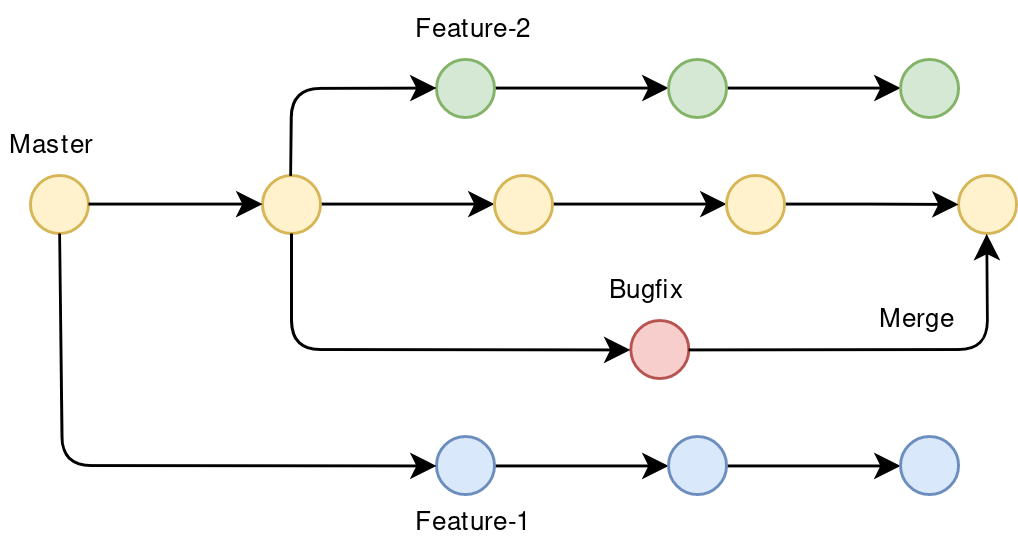
\includegraphics[scale=0.35]{./graphs/git-history-branch}
    \centering
    \caption{A Git commit history tree that shows a history graph with two feature branches and a bug fix that is merged into the master branch.}\label{fig:git-commit-tree}
\end{figure}

As shown in figure~\ref{fig:git-commit-tree} two developers can, for example, create their own branch on which they can work unimpeded.
If they finished their tasks and want to add their work to the master branch, they can now merge their changes.
Git then tries to automatically resolve any conflicts which might have emerged from editing the same lines in a file.
If that is not possible, it marks the conflicts and allows the user to manually correct them.
After this resolution a new \emph{merge commit} is created.
A merge commit represents the merge of changes from two different branches.

With this methodology, it is possible to work with many people or teams on the same project, without accidentally overwriting changes of another developer, whilst maintaining a clear history of all changes in the project.

Another important feature of Git is the possibility to set up a \emph{remote}.
A remote often acts as a centralized repository, developers can \emph{push} their changes to or \emph{pull} changes from other developers.
This principle is called a \ac{cvcs} and is supported by many \acp{vcs}~\cite{version-control}.
It can, for example, be a distinct server, which is attached to some kind of network accessible by the developers.
This feature allows developers to remotely contribute to a project, as long as they have access to the remote's network.
Git also supports several protocols such as \ac{http} or \ac{ssh} to connect to a remote and thereby provide a simple user management layer.


\subsection{Git User Roles}
There exist two roles in Git, the \emph{committer} and the \emph{author}.
Every commit in Git contains the email addresses and the names of those two roles.
The author of a commit is the person who actually contributed the changes in the files.
The committer is the person, who created the Git commit.
This is important to keep track of the original author of the changes.

If one looks at the case of an author contributing code to a project via an email with an attached patch file.
If a maintainer of the project now applies the patch file and commits without setting the author, the information about the original author would be lost.
The collected data of 49 million commits, indicate that in about 89\% the author and the committer are the same person.


\subsection{Internal Representation}~\label{git-internal-representation}
Git's underlying storage and management solution for files is commonly described as a mini \ac{fs}~\cite[p.~9]{book:pro-git}
In the following I will thereby refer to its file management layer as \emph{git-fs} and explain the most important aspects of it.

The representation of a single file in Git is called a \emph{blob} object~\cite[p.~56]{book:pro-git}.
A blob object is a file, which has been added to a \emph{git-fs}.
It is compressed and saved in the \inlinecode{.git/objects} directory under the respective \ac{sha1} hash of the uncompressed file.
As a result, there exists a blob object for every version of every file of the project.

The \ac{sha1} hashing for unique file identifier might seem unsafe at first, but the probability of a \ac{sha1} collision is really low, roughly $10^{-45}$.
In 2017 Google managed to force a collision in a controlled environment, but it is really unlikely to encounter such a collision under normal circumstances~\cite{techreport:sha-collision}.
This characteristic of \ac{sha1} hashing will become quite important in the design of the database later on.

As mentioned in the Section~\ref{git-introduction} Git is used to store the state of a specific directory of an actual \ac{fs}.
To represent a \ac{fs} or to simply bundle multiple Git blob objects together, Git uses the tree object.

A tree object is a file, which has a \ac{sha1} hash reference to all underlying blob and tree objects as well as their names and their \ac{fs} permissions.
To represent a subdirectory, a tree simply holds a reference to another tree object.
With these tools, Git manages to build its own basic representation of a \ac{fs}.

\begin{minted}[linenos]{text}
    100644 blob 11d1ee77f9a23ffcb4afa860dd4b59187a9104e9  .gitignore
    040000 tree ac0f5960d9c5f662f18697029eca67fcea09a58c  expose
    100644 blob 61b5b2808cc2c8ab21bb9caa7d469e08f875277a  install.sh
    040000 tree 8aaf336db307bdcab2f082bd710b31ddb5f9ebd4  thesis
\end{minted}
\begingroup
\captionof{listing}{An example of a Git tree file\label{lst:raw-commit}.}
\endgroup

As stated before the commit is utilized to provide an exact representation of a state of the repository's files and directories.
For this purpose, it holds a reference to the tree object representing the root directory of the project as can be seen in line 1 in Listing~\ref{lst:raw-commit}.
Just as blob objects, the tree and commit files are also stored in the \inlinecode{.git/objects} directory under their respective hash.

\begin{minted}[linenos]{text}
    tree      cd7d001b696db430b898b75c633686067e6f0b76
    parent    c19b969705e5eae0ccca2cde1d8a98be1a1eab4d
    author    Arne Beer <arne@twobeer.de> 1513434723 +0100
    committer Arne Beer <arne@twobeer.de> 1513434723 +0100

    Chapter 2, acronyms
\end{minted}
\begingroup
\captionof{listing}{An example of a Git commit file\label{lst:raw-commit}.}
\endgroup

As you can see in Listing~\ref{lst:raw-commit}, the commit is just another kind of file utilized by Git, which contains some metadata about a repository version:

\begin{itemize}
    \item The reference to a tree object, which represents the root directory of the commit's version of the project.
    \item A reference to one or multiple parent commits, to maintain a version history.
    \item The name and email address of the author.
    \item The name and email address of the committer.
    \item The timestamps with an \ac{utc} offset for the committer and the author.
    \item The commit message. A message with arbitrary text from the committer.
\end{itemize}

The commit is the most important object for this thesis.
It contains crucial information such as the date of the commit as well as the email, which is needed to identify a contributor across several commits.

\subsection{Relevant Features}~\label{git-features}
Git provides a collection of high level abstraction tools to work with its underlying \emph{git-fs}.
In the following, the most important features for data aggregation will be listed and briefly explained.

\begin{description}
    \item[checkout] \hfill \\
        Git allows jumping between different project versions with the \emph{checkout} command.
        Calling \inlinecode{git checkout \$IDENTIFIER} jumps to the commit specified by the variable \inlinecode{\$IDENTIFIER}.
        The identifier, for instance, can be a partial or full \ac{sha1} hash of commit, a branch name or a tag.

    \item[HEAD] \hfill \\
        To mark the current checkout of a repository, Git utilizes a special marker called \emph{HEAD}.
        Due to this feature, it is, for instance, possible to jump to the previous commit in history with \inlinecode{git checkout HEAD\textasciitilde1}.

    \item[diff] \hfill \\
        The \emph{diff} is a tool to compare the state of two different commits in a repository.
        It allows listing all files which changed between those commits as well as showing the exact changes in the files

\end{description}

Git provides many more features, which are not necessarily important for data analysis, but which might need be taken into account when aggregating the data.
In the following, some functionalities will be shown, that can lead to problems or irregularities in the gathered data.

\begin{description}
    \item[force push] \hfill \\
        Git allows pushing to a remote with the \inlinecode{--force} flag, which is called a \emph{force push}.
        This enables the users to rewrite every commit in the whole history tree.
        If another user has the old Git repository version before the force push, they would now be incapable of simply pulling the newest version.
        Instead, they would need to manually checkout the newest commit of the rewritten remote branch and change their branch pointer to the new commit.

    \item[rebase] \hfill \\
        It is possible to \emph{rebase} branches. For instance, a rebase can rewrite the commit history and change the branch point of a branch to another commit.
        This is, for example, a very powerful but also dangerous tool, as it also implicitly changes the timestamps of the commits of the rebased branch.

    \item[filter-branch] \hfill \\
        In case somebody pushes a huge file, which significantly increases the size of the repository, or adds a file with secret information, such as a password file, Git provides the \emph{filter-branch} command.
        The filter-branch command removes a specified file from every commit in the history and thereby rewrites the history to the point, where this file was added to the repository.
        This command leads to similar problems as the rebase command since it can severely change the history of a repository.

\end{description}


\section{Data source}\label{data-source}
The acquisition and clean-up of data was the biggest initial task of this thesis.
Selecting a data source was a crucial step, as good data for analysis and evaluation is the backbone of this thesis.
This section will list all requirements in detail and evaluate why I chose to use Github as a data source.
Furthermore, some functionalities of Github will be explained and a brief overview of the data provided by Github's \ac{api} will be given.


\subsection{Requirements}\label{requirements}
The data source had to satisfy as many requirements as possible, as specified in Section~\ref{attack-goals}.

To accomplish a meaningful analysis one needs a sufficient amount of commits.
For instance, it is necessary to have a few commits per weekday over a timespan of at least a month for a simple sleep rhythm analysis.
If there are only 20 commits for a user over the past month there is probably not enough data for a representative analysis.
To gather as many commits as possible I had to get access to as many repositories, to which the targeted users contributed to, as possible.
Thereby the data source has to provide a way to dynamically explore repositories around a single user or company.

For analysis of companioned persons as described in Section~\ref{attack:industrial-spy} it is crucial to find users, who are likely to know each other.
Optimally the data source provides a functionality for users to actively mark other users as their friends or colleagues.

To attack a company or to spy on company members, as described in Section~\ref{attack:employer-monitoring}, the best case scenario would be to have full access to all repositories owned by the company.
The data source thereby needs to provide some kind of representation for a company.
Ideally, there should also be a list of all company members for evaluation purposes of data mining findings.


\begin{itemlist}{A summary of the requirements to the data source:}
    \item Real world data
    \item Large amount of repositories
    \item Access to all commits of each repository
    \item Access complete metadata for each commit
    \item Email address to user association
    \item Methods to discover repositories a user contributed to
    \item Methods to discover possibly companioned contributor
    \item A representation of a company
    \item Access to members of a company
\end{itemlist}


\subsection{Github}\label{github}
I decided to use Github as a data source, as it is not only convenient to find \acp{url} for cloning repositories but also provides solutions for most of the other requirements.
It hosts one of the biggest collections of open-source projects~\cite{techreport:how-github-conquered} with 64 million repositories, 24 million users and 1,5 million organizations~\cite{article:github-statistics}.
Github also provides a well-documented \ac{api} for querying its metadata and there are libraries for most major languages, which provide an abstraction layer for this \ac{api}.
This \ac{api} is publicly available and can be used by anyone registered on Github.

For instance, Gitlab, one of Github's competitors, has much fewer data to offer.
Gitlab does not provide detailed usage statistics, but they state that they only host about 100000 organizations, which is remarkably less than Github~\cite{article:gitlab-help}.

On the other hand, one of the downsides of using Github is, that we do not have access to all metadata.
For example, the full list of members for organizations is often inaccessible, as users need to actively opt-in to be publicly displayed as a member of the organization.
The internal team structures of organizations are not visible at all, as one needs to be a member of the organization to access those.
Another problem are dangling email addresses, which are not related to any account anymore.
All commits made with such an email address cannot be used any more for any analyses that require a user to commit relationship.
But even though some ground truth is missing, I decided to use this approach as it still was the most promising way to gather as much data and real-world noise as possible, compared to other open-source hosting services.

\begin{figure}[H]
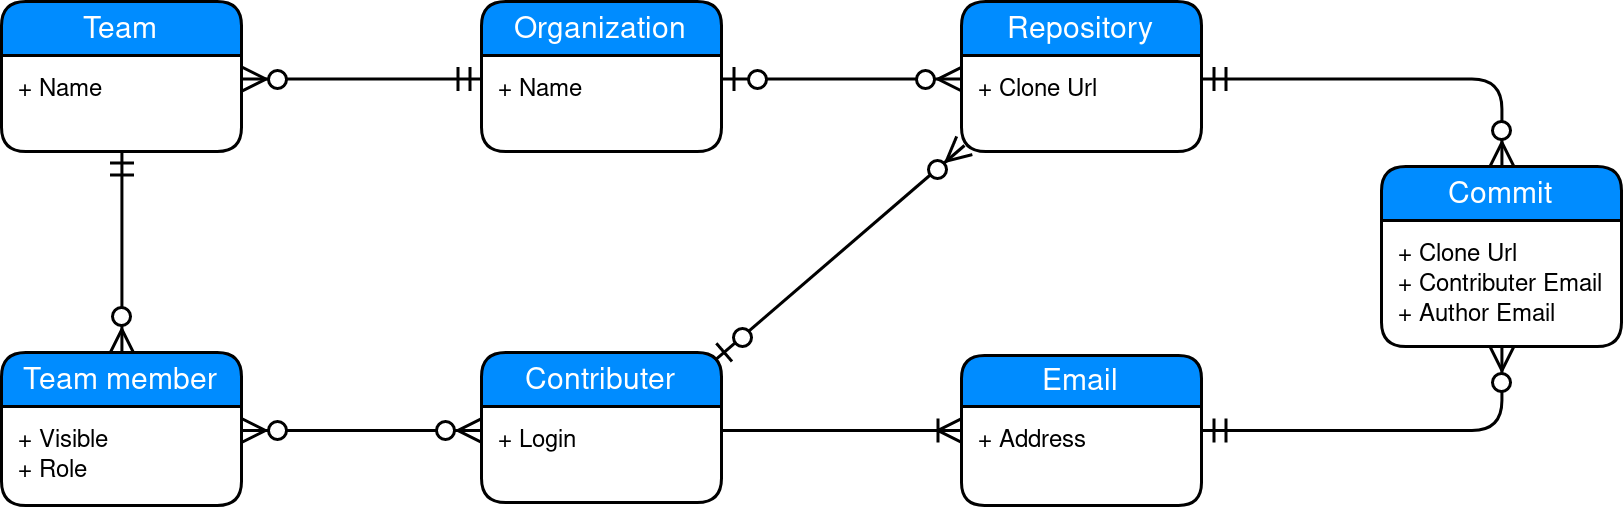
\includegraphics[scale=0.27]{./graphs/github-data-structure}
\centering
\caption{A simplified visualization of Github's internal relationships between the most important objects in Crow's foot notation.}\label{fig:github-relationship}
\end{figure}

\subsection{Github's Features}\label{github-features}
In the following I will explain some of the features provided by Github, that cover the requirements listed in Section~\ref{requirements}.
Github offers some features, which, for example, are convenient to finding repositories a specific user contributed to or to find contributors hwo likely personally know each other.

\begin{description}
    \item[Stars] \hfill \\
        A very crucial feature is \emph{starring}. Every user has the possibility to star a repository to show appreciation or interest in this specific project.
        Hence popular repositories usually have a comparatively large number of stars. For instance, the Github Linux kernel mirror has a star count of over 58000~\footnote{`Linux kernel source tree' Github.com, https://github.com/torvalds/linux (accessed, 24.04.2018)}.
        Even though Github allows to query all repositories, which are owned or forked by a user, their \ac{api} does not provide a method to get all repositories a user ever contributed to.
        However, Github provides an endpoint to query all starred repositories of a user.
        In case a user stars a repository he contributed to, whilst not owning it, it is now possible to get this repository with this feature.
        Of course, it is still not a reliable way to get all repositories a user ever contributed to, but it is a viable approach to get at least a few of them.

    \item[Follower] \hfill \\
        Another important feature is \emph{following}.
        Every user can follow any other user to get informed, when they do specific things, like creating new repositories or starring repositories or to simply show interest in or respect for their work.
        By getting all followed or following users, one might catch some friends of the user.
        It is also possible that a user follows the owner of a repository he contributed to.
        By using this feature it is thereby possible to get some additional repositories they contributed to, as well as some friends of the user.

    \item[Organizations] \hfill \\
        The last feature is \emph{organizations}.
        An organization is used to host projects under an account, that is not necessarily led by a single natural person, but rather supports roles with different permissions and team structures.
        Github allows querying all repositories of an organization via their \ac{api}.
        This enables us to link an organization to its owned repositories and as a result to perform analyses for users on a specific organization repository subset.

        Generally, organizations provide us with some important ground truth, even though the information might not be complete.
        Despite not knowing all members of an organization, we still get some useful information to estimate the tendency of precision of our knowledge extraction algorithms.
\end{description}


\section{Data Aggregation}\label{aggregator}
As mentioned in Section~\ref{github}, I decided to use Github as my primary data source and to utilize their \emph{Github APIv3} for this purpose.
The aggregator and analysis program written for this thesis is named \emph{Gitalizer}.
In this section, I will explain the technologies and methods used in the data aggregation process, the database structure and the interaction with Github's \ac{api}.
In the end, some problems which occurred during the data collection will be shown as well.


\subsection{Existing Solutions}
There are of existing solutions for accessing and collecting Git metadata.
In the following, the practicability of these solutions is evaluated based on our requirements.

\subsubsection{GHTorrent}
The \emph{GHTorrent} project aims to provide Github's metadata to elude the limitations of Github's \ac{api} rate limiting~\cite{inproceedings:ghtorrent}.
It provides representations for followers and commits, as well as organizations and organization members, but some crucial pieces of information are missing.
GHTorrent only stores the main email address of a user and does thereby not support the handling of multiple emails, as commits are directly assigned to their respective Github user id.
Commits miss information about additions and deletions in lines of code, which implicates that each commit would need to be scanned by a separate program again.
Furthermore, GHTorrent does not have the concept of \emph{starring}, which makes it hard to reduce the number of considered repositories to a manageable size.
Their database provides about 4~\ac{tb} of data according to their website, which is too much information without the possibility of specifying a precise subset of data~\footnote{`The GHTorrent project' ghtorrent.com, http://ghtorrent.org/ (accessed, 05.05.2018)}.
It provides a vast amount of data, but at the same time, it cannot be ensured, that the data is as complete as possible for a specific user.
Modifying the GHTorrent code base and extending their database schema has thereby been judged as impractical.

\subsubsection{ghcrawler}
Microsoft provides an open-source crawler called \emph{ghcrawler}, which is supposed to continuously fetch data from Github~\footnote{`Github crawler' github.com, http://github.com/ (accessed, 05.05.2018)}.
Sadly their documentation is very incomplete and after diving into their source code, it appears that their crawler is for Github entities only and not for the underlying data of Git repositories.

\subsubsection{Alitheia-Core}
\emph{Alitheia-Core} is a Java data collector for Git repositories.
It is not actively maintained for more than three years and their documentation website is offline.
Using this library seemed unpromising and unfeasible.

\subsubsection{RepoDriller}
The \emph{RepoDriller} project aims to support researchers by providing easy access to repository data from Github~\footnote{`A tool to support researchers on mining software repositories studies' github.com, http://github.com/ (accessed, 05.05.2018)}.
Despite providing a good solution for getting all necessary information from a repository, it provides no way to explore Github using \emph{stars} or \emph{following}.
These features, as well as the assignment of emails to a contributor via the Github \ac{api}, would need to be added.
As the program is also written in Java and I am no longer familiar with the language and its ecosystem, I decided to stick to writing my own solution.

\subsection{Database}\label{gitalizer-database}
To store the gathered Information I chose a \ac{sql} based solution.
PostgreSQL provides excellent tools to ensure a high consistency in your database, namely check constraints, as well as great support for working with times, time zones and locations.
The \ac{sql} database is used in combination with the \ac{orm} library \emph{SQLAlchemy}.

The basic schema created for the purpose of this thesis consists of five \ac{orm} models.
A model for commits, emails, repositories, contributors, and organizations has been created.
The latter is only important to validate results and is not actually used for knowledge discovery, as this is Github specific data.

\begin{figure}[H]
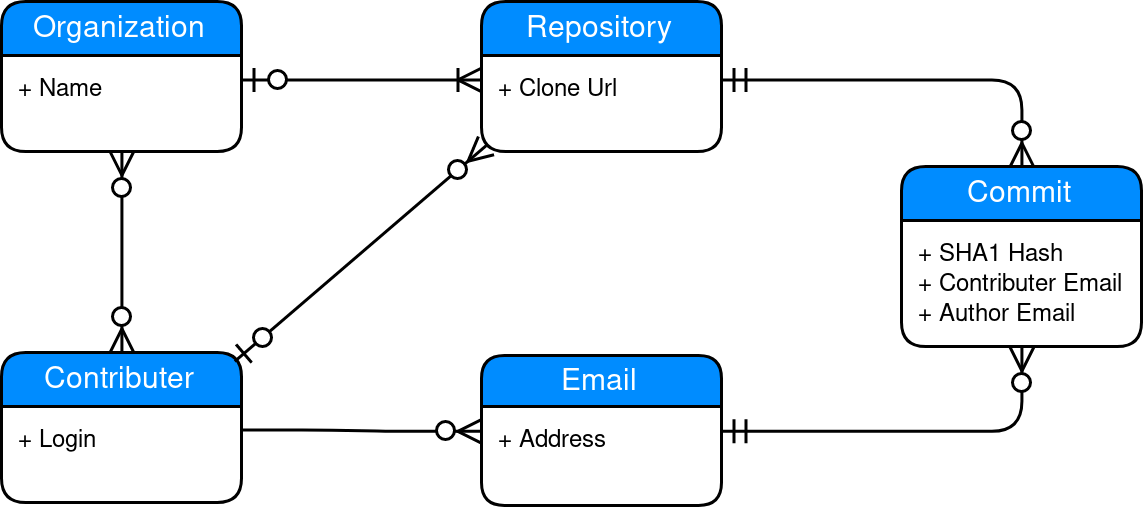
\includegraphics[scale=0.3]{./graphs/gitalizer-data-structure}
\centering
\caption{The relationships between Gitalizer's most important database objects in Crow's foot notation.}\label{fig:gitalizer-relationship}
\end{figure}

Every commit of each repository is saved in the database along with its \ac{sha1} hash and the two email addresses as in Listing~\ref{lst:raw-commit}.
It is important to note that there is a many-to-many relationship in figure~\ref{fig:gitalizer-relationship} between commits and repositories.
This feature prevents duplication of the same commits from forked repositories.
It is, for instance, a common practice to create a fork of a repository to develop without intervening with the main Git repository of the project.
As described in Section~\ref{git-internal-representation} the probability of a \ac{sha1} collision is highly improbable.
By exploiting this feature, it is possible to enforce a unique constraint on the commit hash column, assuming that any duplicated commit hash actually results from a forked or copied repository.
The formula for calculating the probability of such a collision is as follows, where $p$ is the probability of collision, $n$ is the number of different hashes and $b$ is the size of the hash in bytes:

\begin{equation}\label{eq:collision-probability}
    p \leq \frac{n(n-1)}{2} * \frac{1}{2^{b}}
\end{equation}

Without this mechanism, it could be possible that the same commit of a contributor could be used multiple times as a result of repository forking.
After collecting 43 million commits from Github and actively ignoring obvious project forks, there are still 49 million references between commits and repositories.
This means that about 13\% of gathered commits result from forked repositories which cannot easily be identified as such.
Considering Formula~\ref{eq:collision-probability}, the probability of a collision for 49 million hashes on the 160 bit \ac{sha1} hash would be about $8.21 * 10^{-34}$.

As stated above each commit is also saved with its respective email addresses.
There exists a one-to-many relationship between contributors and emails since every contributor can obtain an unlimited amount of email addresses.
It is necessary to connect all email addresses to a specific contributor, to unambiguously assign all commits to their respective contributor.
This relationship does not have a \inlinecode{NOT NULL} constraint as it happens quite often that an email address cannot be assigned to any person.
Looking at the collected data it appears that roughly 20\% of all collected email addresses from Github are no longer connected to an active user.

As stated in Section~\ref{github-features} Github provides a way to organize several people in organizations and teams.
As one of the potential goals of this thesis is to see if it is possible to detect members of an organization in open-source projects, a model for organizations has been created as well.
This data can then be used to check the results of this research's results.


\subsection{Gitalizer}
The Program written for this thesis features data aggregation, preprocessing, knowledge extraction and visualization.
Gitalizer uses a PostgreSQL database for data storage and data consistency checks as described in~\ref{gitalizer-database}.
For interaction with the Github \ac{api} the \emph{PyGithub} library is used.
It provides a convenient abstraction layer for requests and automatically maps \ac{json} responses to \emph{Python} objects.

The data aggregation module of Gitalizer is capable of several approaches for gathering data.
In the following, I will explain those approaches in detail.

\begin{description}
    \item[Git repository]\label{stand-alone-repository-scan} \hfill \\
        Gitalizer can scan any Git repository from a \ac{ssh} or \ac{http} \acs{url}, as long as the user used by Gitalizer has access to it.
        The repository is cloned into a local directory.
        After the cloning is done, the actual scanning process begins.
        During the scan, the \inlinecode{HEAD} of the current default branch for this repository is checked out and every from the \inlinecode{HEAD} downwards reachable commit of the Git history is scanned.
        The program saves all available metadata for each commit in its database, which are emails, timestamps as well as additions and deletions to the project in lines of code.

        After this scan, a lot of information is still missing.
        There exists no unique identifier of an author or committer since names may change or can be ambiguous and a single person can have multiple email addresses.
        The problem with the simplicity of Git is that there exists no concept of a user.
        Thereby we cannot easily link several email addresses to a specific contributor without additional metadata.


    \item[Github Repository]\label{github-repo-scan} \hfill \\
        To tackle the problem of missing metadata in the previous approach, I used the Github \ac{api} to get some of the missing metadata.
        The general approach is the same as in the previous scan method.
        At first, the repository is cloned and locally scanned.
        However, a request is issued to Github every time an email is found, that is not already linked to a contributor.
        Github allows linking multiple email addresses with a single user account and automatically references the respective user in their own \ac{api} commit representation.
        With this additional metadata, we gain ground truth about the identity of an author or committer.

        Anyway, this approach does not work if the user of a commit removes the email, which has been used for the commit, from their account or if the user completely deletes their account.
        If this happens and the email contributor relationship has not already been created in a previous scan, there is nothing that can be done and those commits need to be handled later on during the preprocessing of the data.

    \item[Github User]\label{github-repo-scan} \hfill \\
        While trying to get all repositories of a specific user, a new functionality has been added, which highly utilizes the Github \ac{api}.
        At first, several requests are issued to get all repositories of the specified user, as well as all starred repositories of this user.
        During the repository exploration, every relevant repository is added to a shared queue, called the ``repo-queue'', which is then processed by a multiprocessing pool of workers.
        Each worker process continuously pops entries from the ``repo-queue'' and scans every single repository as described in the previous approach.


    \item[Connected users and organizations]\label{github-repo-scan} \hfill \\
        For detection and analysis of connections between contributors over multiple repositories, additional user repository discovery, as described in Section~\ref{requirements}, has been added to Gitalizer.
        Gitalizer is able to achieve this by not just scanning a single user, but also scanning the repositories of all following and followed users as described in the previous approach.
        For this task, two different worker pools are utilized.
        The user discovery pool is initialized with a shared queue, called ``user-queue'', with all users we need to look at.
        This worker pool simply searches for relevant repositories of each user and passes the repository \ac{url} to the second shared queue.
        The second worker pool then processes the ``repo-queue'' as described in the approach for Github repositories.

        For organizations, it is nearly the same approach.
        Initially, all repositories, which are owned by the organization, are added to the ``repo-queue''.
        All publicly visible organization members are then added to the ``user-queue'' and processed as described above.
\end{description}


\subsection{Database Optimization}
As the database kept growing, it became the bottleneck in the aggregation process several times.
As a result, adjustments in the database schema, PostgreSQL parameter tweaking and a migration to better hardware were necessary.
The first considerable slowdown occurred after reaching about 12~\acp{gb} of data.
At this stage, the database \ac{io} operations took longer than the actual aggregation process and the whole machine started to become unresponsive because of high \ac{io} load.

The performance of the database then needed to be continuously tweaked in several steps.
The first countermeasure was the reduction of commits using deduplication by using the features of the \ac{sha1} hash as stated in Section~\ref{gitalizer-database}
Ignoring forked repositories reduced the number of entries in the relation table between commits and repositories by another 26\%.

Other performance boosts were achieved by disabling or loosening several fail-safe mechanisms of PostgreSQL, namely `synchronous commit' and `write-ahead' parameter, which are designed to prevent data loss on a system crash.
As there is no important or critical data handled, it was acceptable to pass on these mechanisms and to trade safety for performance.

\begin{figure}[H]
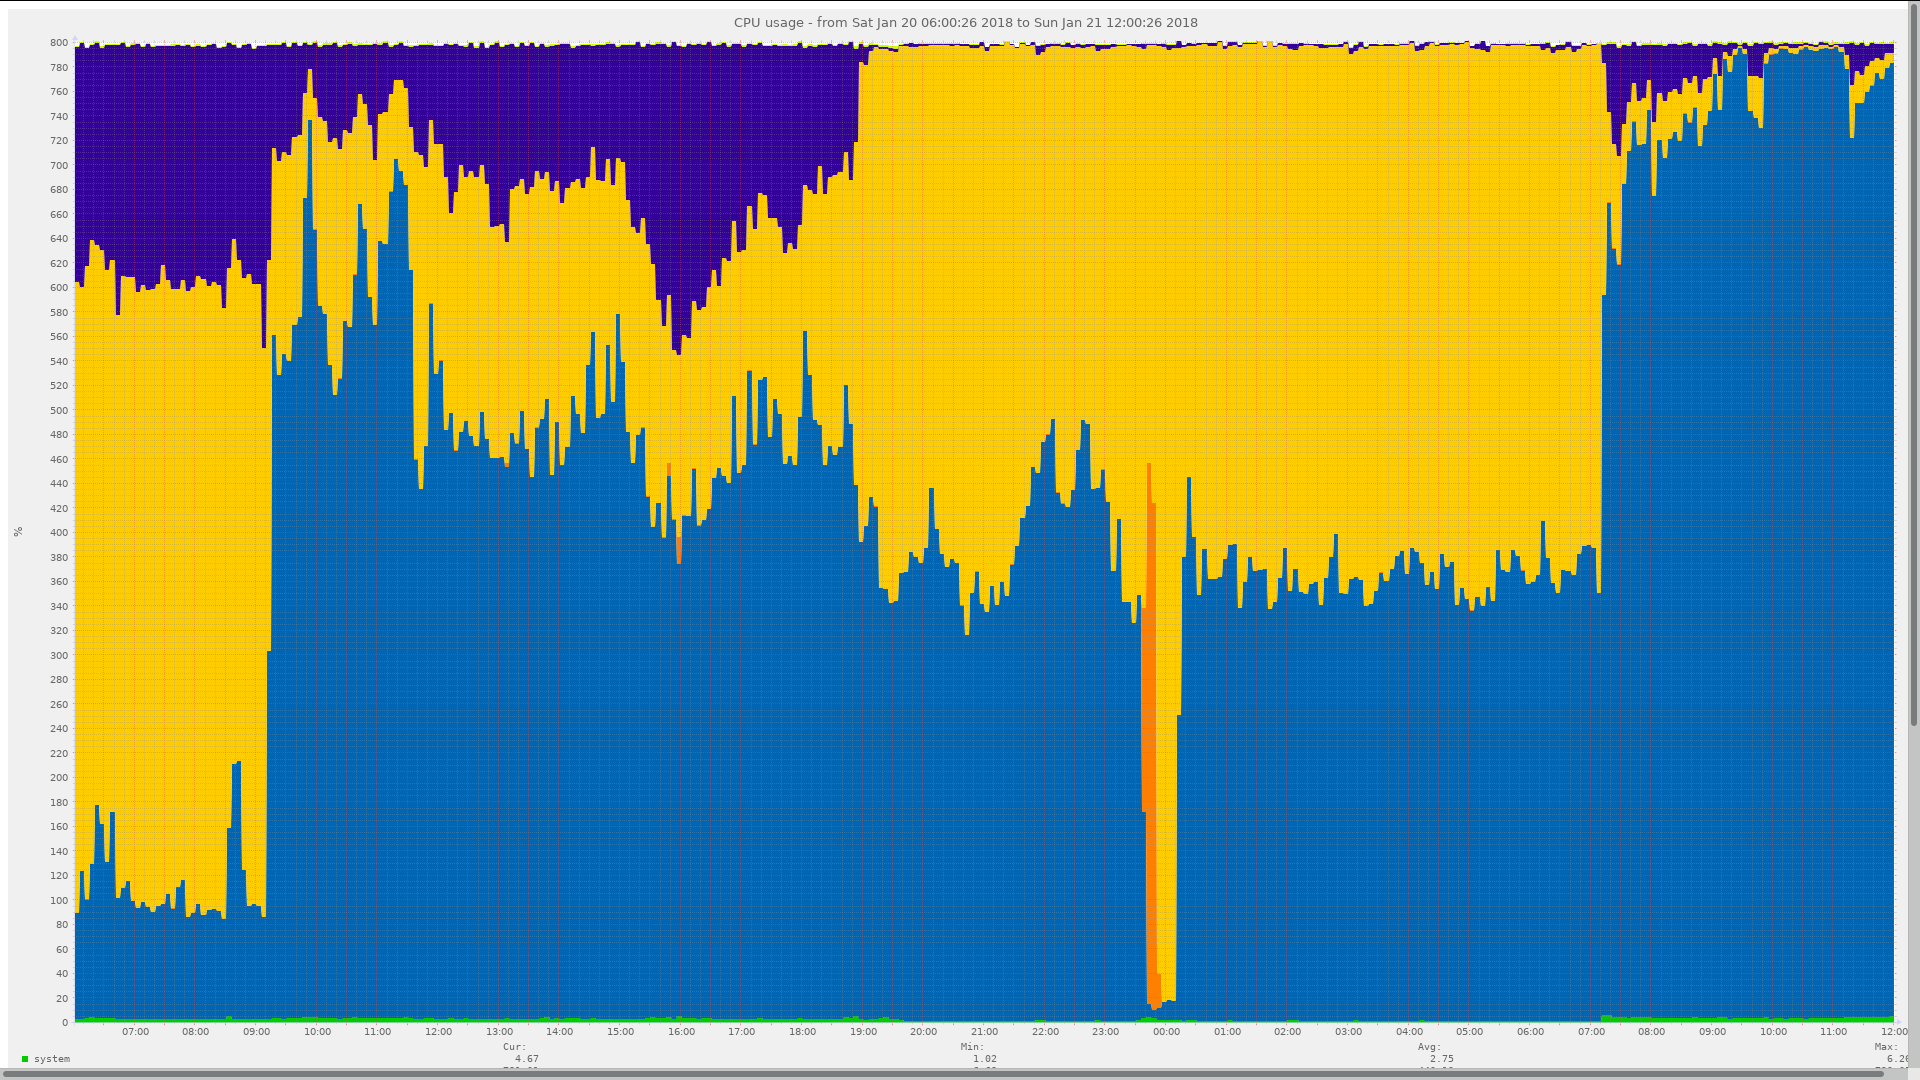
\includegraphics[scale=0.22]{./graphs/server-graphs/query-refactoring}
\centering
\caption{The \ac{cpu} load of the aggregation server before and after query and cache optimization.
The light blue area represents the \ac{cpu} percentage actually used for computation.
The dark blue area represents the amount of \ac{cpu} idle time due to \ac{io} load.
At the beginning of the graph the server was partly unresponsive due to high \ac{io} wait.
At the right side of the graph the \ac{io} load is significantly reduced after some optimizations.}\label{fig:cpu-load}
\end{figure}

After renting a root server and deploying Gitalizer onto it, the aggregation process worked really well, until the database size hit about 25~\ac{gb}.
In Figure~\ref{fig:cpu-load} the overall \ac{cpu} load right before optimizing several \ac{sql} queries, by caching intermediate results and increasing the cache size of PostgreSQL, can be seen.
The dark blue represents the \ac{io} wait time while the light blue represents the actually used processor capacity by the aggregator.
Due to complex and numerous \ac{sql} queries the server became partly unresponsive and the aggregation process began to stall.

After many improvements, the server can now run with 16 worker threads and roughly 38~\ac{gb} of data without any signs of slowdown whilst using the rate limit to capacity.


\subsection{Incremental Aggregation}
To ensure a constantly up to date database, Gitalizer needed to be capable of fast rescans of repositories.
The initial scan of a repository always includes cloning, scanning the whole repository and writing it into the database.
After a repository is scanned completely at least once, it is marked as such and will never by completely scanned again.
All following runs then only clone the repository and scan the newest unknown commits.
These are discovered by performing a breadth-first search until no new commits can be found.

\begin{figure}[H]
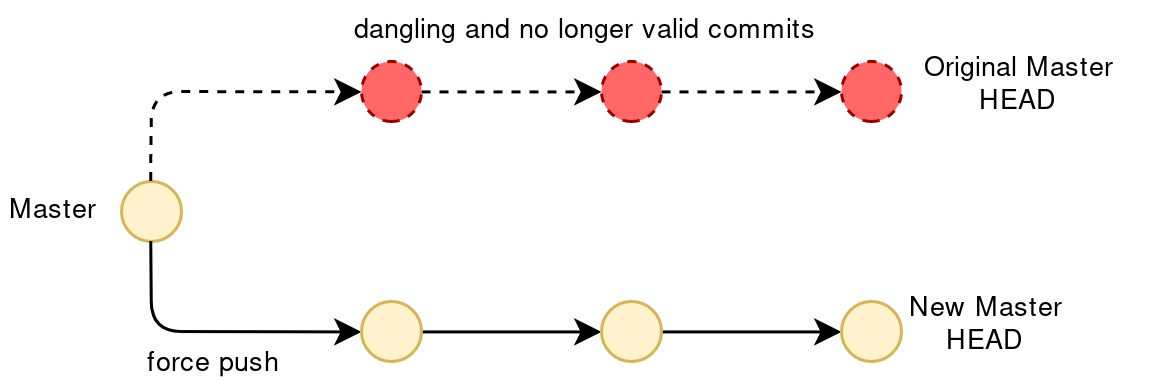
\includegraphics[scale=0.3]{./graphs/git-history-rewrite}
\centering
\caption{This figure shows an example of a Git history tree which master branch's history has been rewritten by a force push.}\label{fig:truncated-git-history}
\end{figure}

As explained in Section~\ref{git-features} it is possible to rewrite commits and force push them.
This scenario needs to be explicitly handled since force pushes can completely alter the history of a Git repository, which can subsequently lead to a split in the Git history and leave dangling commits.
As the complete history of a repository is stored in the database, Gitalizer needs to detect a force push by walking down the Git history tree until it finds known commits.
If any of these commits have children, which are not in the newly scanned commits, a force push took place and the old commit history has to be flagged as such since it is now outdated and irrelevant.
An example scenario can be seen in Figure~\ref{fig:truncated-git-history}, where all red commits represent the old commit history, which needs to be truncated.


\subsection{Problems}
During the development of the data aggregator, I experienced a few problems and edge cases that needed to be handled.
The earliest and most delaying problem was the rate limit of the Github \ac{api}, which is limited to 5000 requests per hour.
Beside this rate limiting, there also is an abuse detection mechanism, that triggers if too many requests are fired in a short amount of time.
The solution for this problem resulted in various workarounds, which include random wait times to detain those mechanisms from triggering.

The first version of the aggregator did not clone and scan the repository locally, but rather gathered all information from the Github \ac{api} endpoints.
This approach worked well until the aggregator hit the official repository of \emph{Nmap}, which had about 11.000 commits and took over three hours to scan.
Soon I realized that this would severely slow down my research and I then started to continuously minimize the amount of \ac{api} calls issued by Gitalizer, to avoid waiting for a reset of the previously mentioned \ac{api} limit.
A connected user scan of my own Github account led to about 600.000 commits and took about one and a half day on the final working version of Gitalizer, to provide you with a reference of scale.

After implementing multiprocessing, I managed to hit the rate limit again, as I was now issuing requests to the \ac{api} with multiple threads.
To fix this issue I implemented a wait and retry wrapper around every single function call or object access, that triggered a call to the Github \ac{api}.
Afterward, the aggregator was capable of running multiple days without worker processes silently dying or finishing with incomplete data.

Fine tuning the edge cases and the handling of the \ac{api} took about 3 months since there were many problems such as unpredictable error responses from Github, missing data in queries or simply unknown or broken encodings in Github's metadata.

A big throwback became apparent as I discovered that PostgreSQL automatically normalizes \ac{utc} timestamps with any offset to the \inlinecode{UTC +0} timezone.
As a result of this normalization, the exact time of the commit admittedly stays the same, but the crucial metadata about the offset is lost.
As a consequence, the commit model needed to be adjusted, as the \ac{utc} offset had to be stored explicitly, and the whole commit aggregation process was started from scratch.

Another problem occurred during the local scanning of the repositories.
The \emph{libgit2} library, used for interaction with Git, issued \emph{stat} Linux syscalls during a diff operation for each file, which changed between the compared commits, to check if there were any local uncommitted changes.
Anyhow the locally scanned repositories were cloned in \emph{bare} mode.
This means that there exists no project root directory, but rather only the git internal representations of those files, which makes the behavior stated above unnecessary and unwanted.
As a result, all processes slowed severely down due to high \ac{io} wait times, because of a huge amount of stat syscalls on non-existent files.
Luckily after reporting the issue~\footnote{`Unnecessary syscalls on bare repository' github.com, https://github.com/libgit2/libgit2/issues/4480 (accessed, 25.04.2018)} it was resolved in a week and I was able to continue developing with my own compiled version of the libgit2 library.



\chapter{Attack Implementations}~\label{implementation}
After collecting all necessary data as shown in Chapter~\ref{data}, this chapter now attends to the analysis of this data.
The approach for several attacks, as listed in Section~\ref{attack-goals} will be presented and their attack goals recapitulated.
The possible applications for the gained knowledge will be stated and the implementation of and requirements to the respective algorithm will be explained for each attack.

\section{Holiday and Sick Leave Detection}

Figure~\ref{fig:missing-time} shows the analysis of an employee for their employer's repositories.
The y-axis represents the additions and deletions of commits, the x-axis represents the week of the respective year.
For better verification and evaluation of the results, a scatter plot with the additions and deletions of each commit has been added on top of individual miss-out graphs.

\begin{figure}[h]
    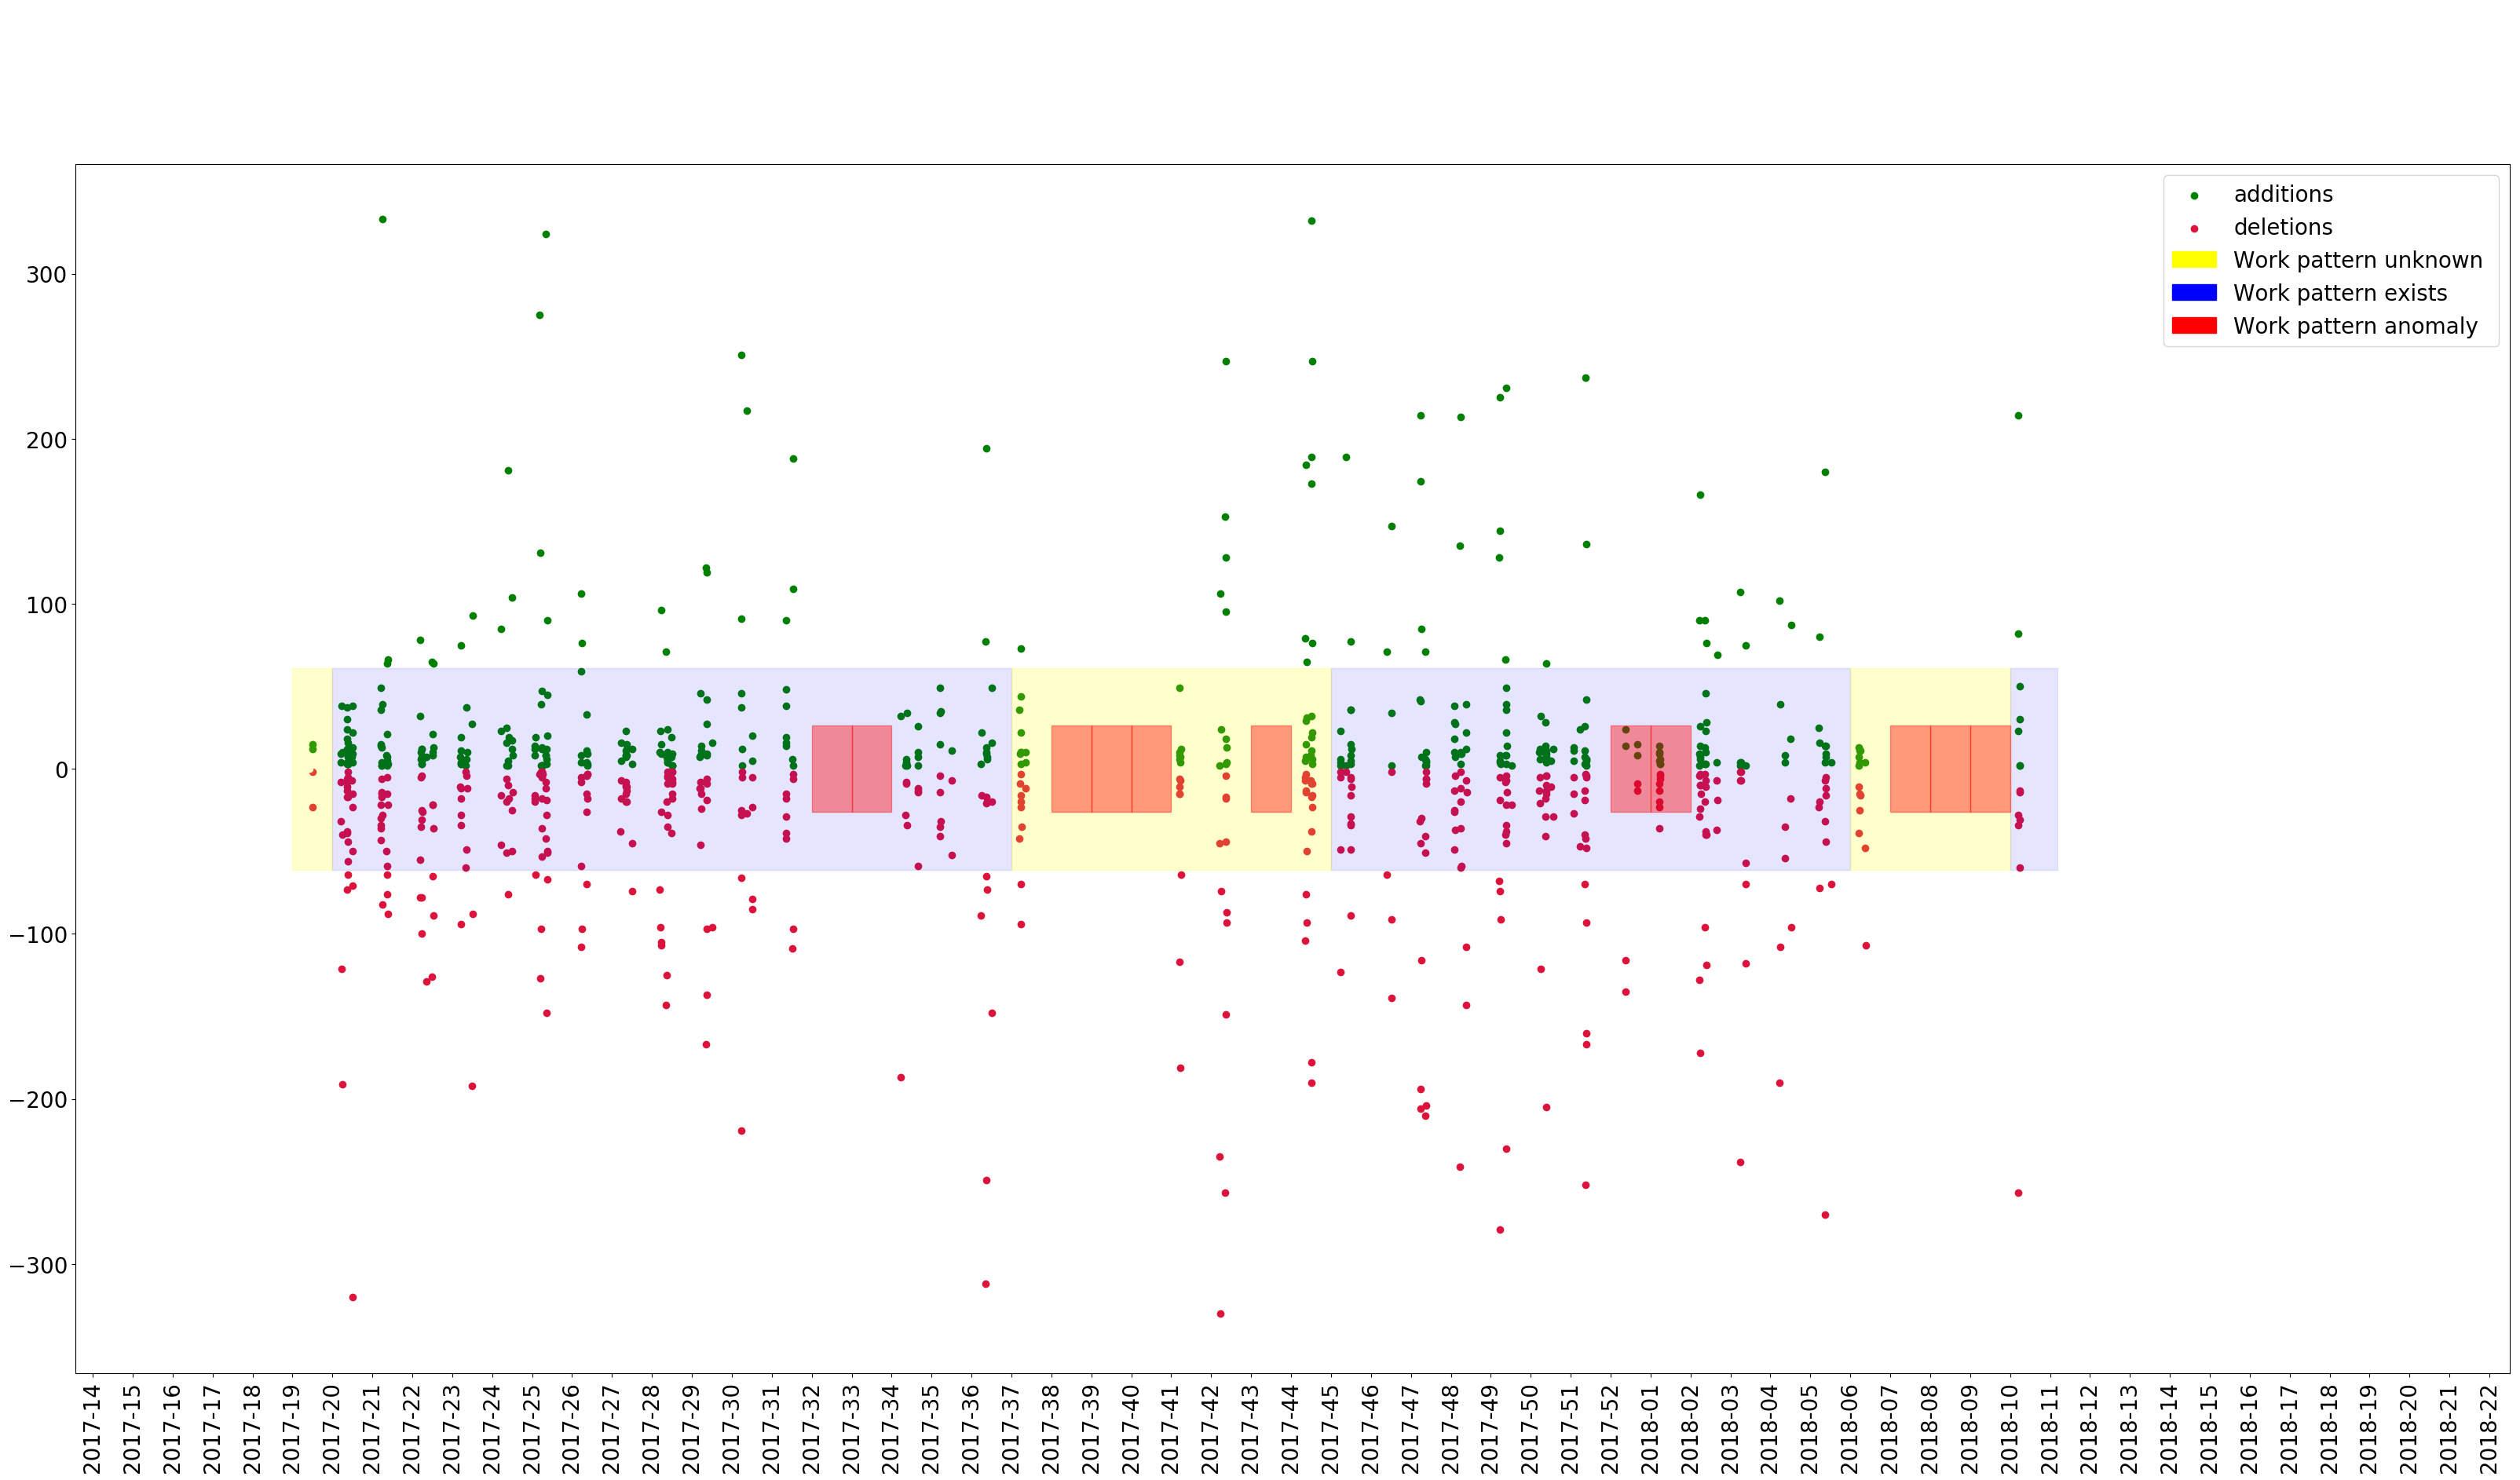
\includegraphics[scale=0.19]{./graphs/analysis/work-time-analysis}
    \centering
    \caption{
        The work time analysis of an employee.
        Blue sections are time spans in which the target has a consistent reoccurring week work pattern.
        Yellow sections show irregularities in their week work pattern.
        Red blocks are miss-out anomalies detected by the algorithm, which indicate holiday or sick leave.
    }\label{fig:missing-time}
\end{figure}

The evaluation of this algorithm turned out to be quite difficult, as there is no publicly available information about sick leave or holiday.
For the purpose of this thesis, I was allowed to use anonymous statistics of a company with a test group of five developing employees.

After scanning and analyzing the company's repositories, a survey has been conducted, for which each employee had to look at their visualized miss-out graph and check whether there are any wrong or missing detections.

The algorithm successfully managed to find all sick leave and holiday-related miss-outs in all cases.
However, there were three false positive cases.
Firstly a developer did work related research and did thereby not commit as regularly as usual, which was then detected as a miss-out.
Secondly, a developer contributed to repositories, which are not owned by the employee.
As a result, two weeks were marked as miss-out.
Thirdly there were two developers, that contributed to a branch, but their work has not been merged into the master branch yet, hence the commits were not being scanned yet.
This particular problem can be solved by not only scanning the master branch but also all other branches, however, this adds a lot of complexity to the continuous mining process and has thereby not been implemented yet.
Anyway, this problem only seems to occur in the latest weeks.

A not intended side effect of detecting prototypes is that the algorithm not only detected anomalies, such as sick leave or holiday, but also found inconsistencies in the work routine.
For instance between week 37 to 45 in Figure~\ref{fig:missing-time}, a developer was forced to reduce their working hours due to legal questions and continuously shifted hours and working days for several weeks.
It is hard to interpret those inconsistencies without more contextual information, but nevertheless, it provides the fact that something happened during this time.

The conducted survey also included a question about the precision of these inconsistencies.
In the case of three developers, the inconsistencies perfectly matched real-world occurrences in their work behavior.
In the two remaining cases, there were a few inconsistencies the developers could not explain, even though there definitely were inconsistencies in their commit pattern.
But those inconsistencies could be explained by the fact that those developers were working on flexible work time.

\begin{figure}[h]
    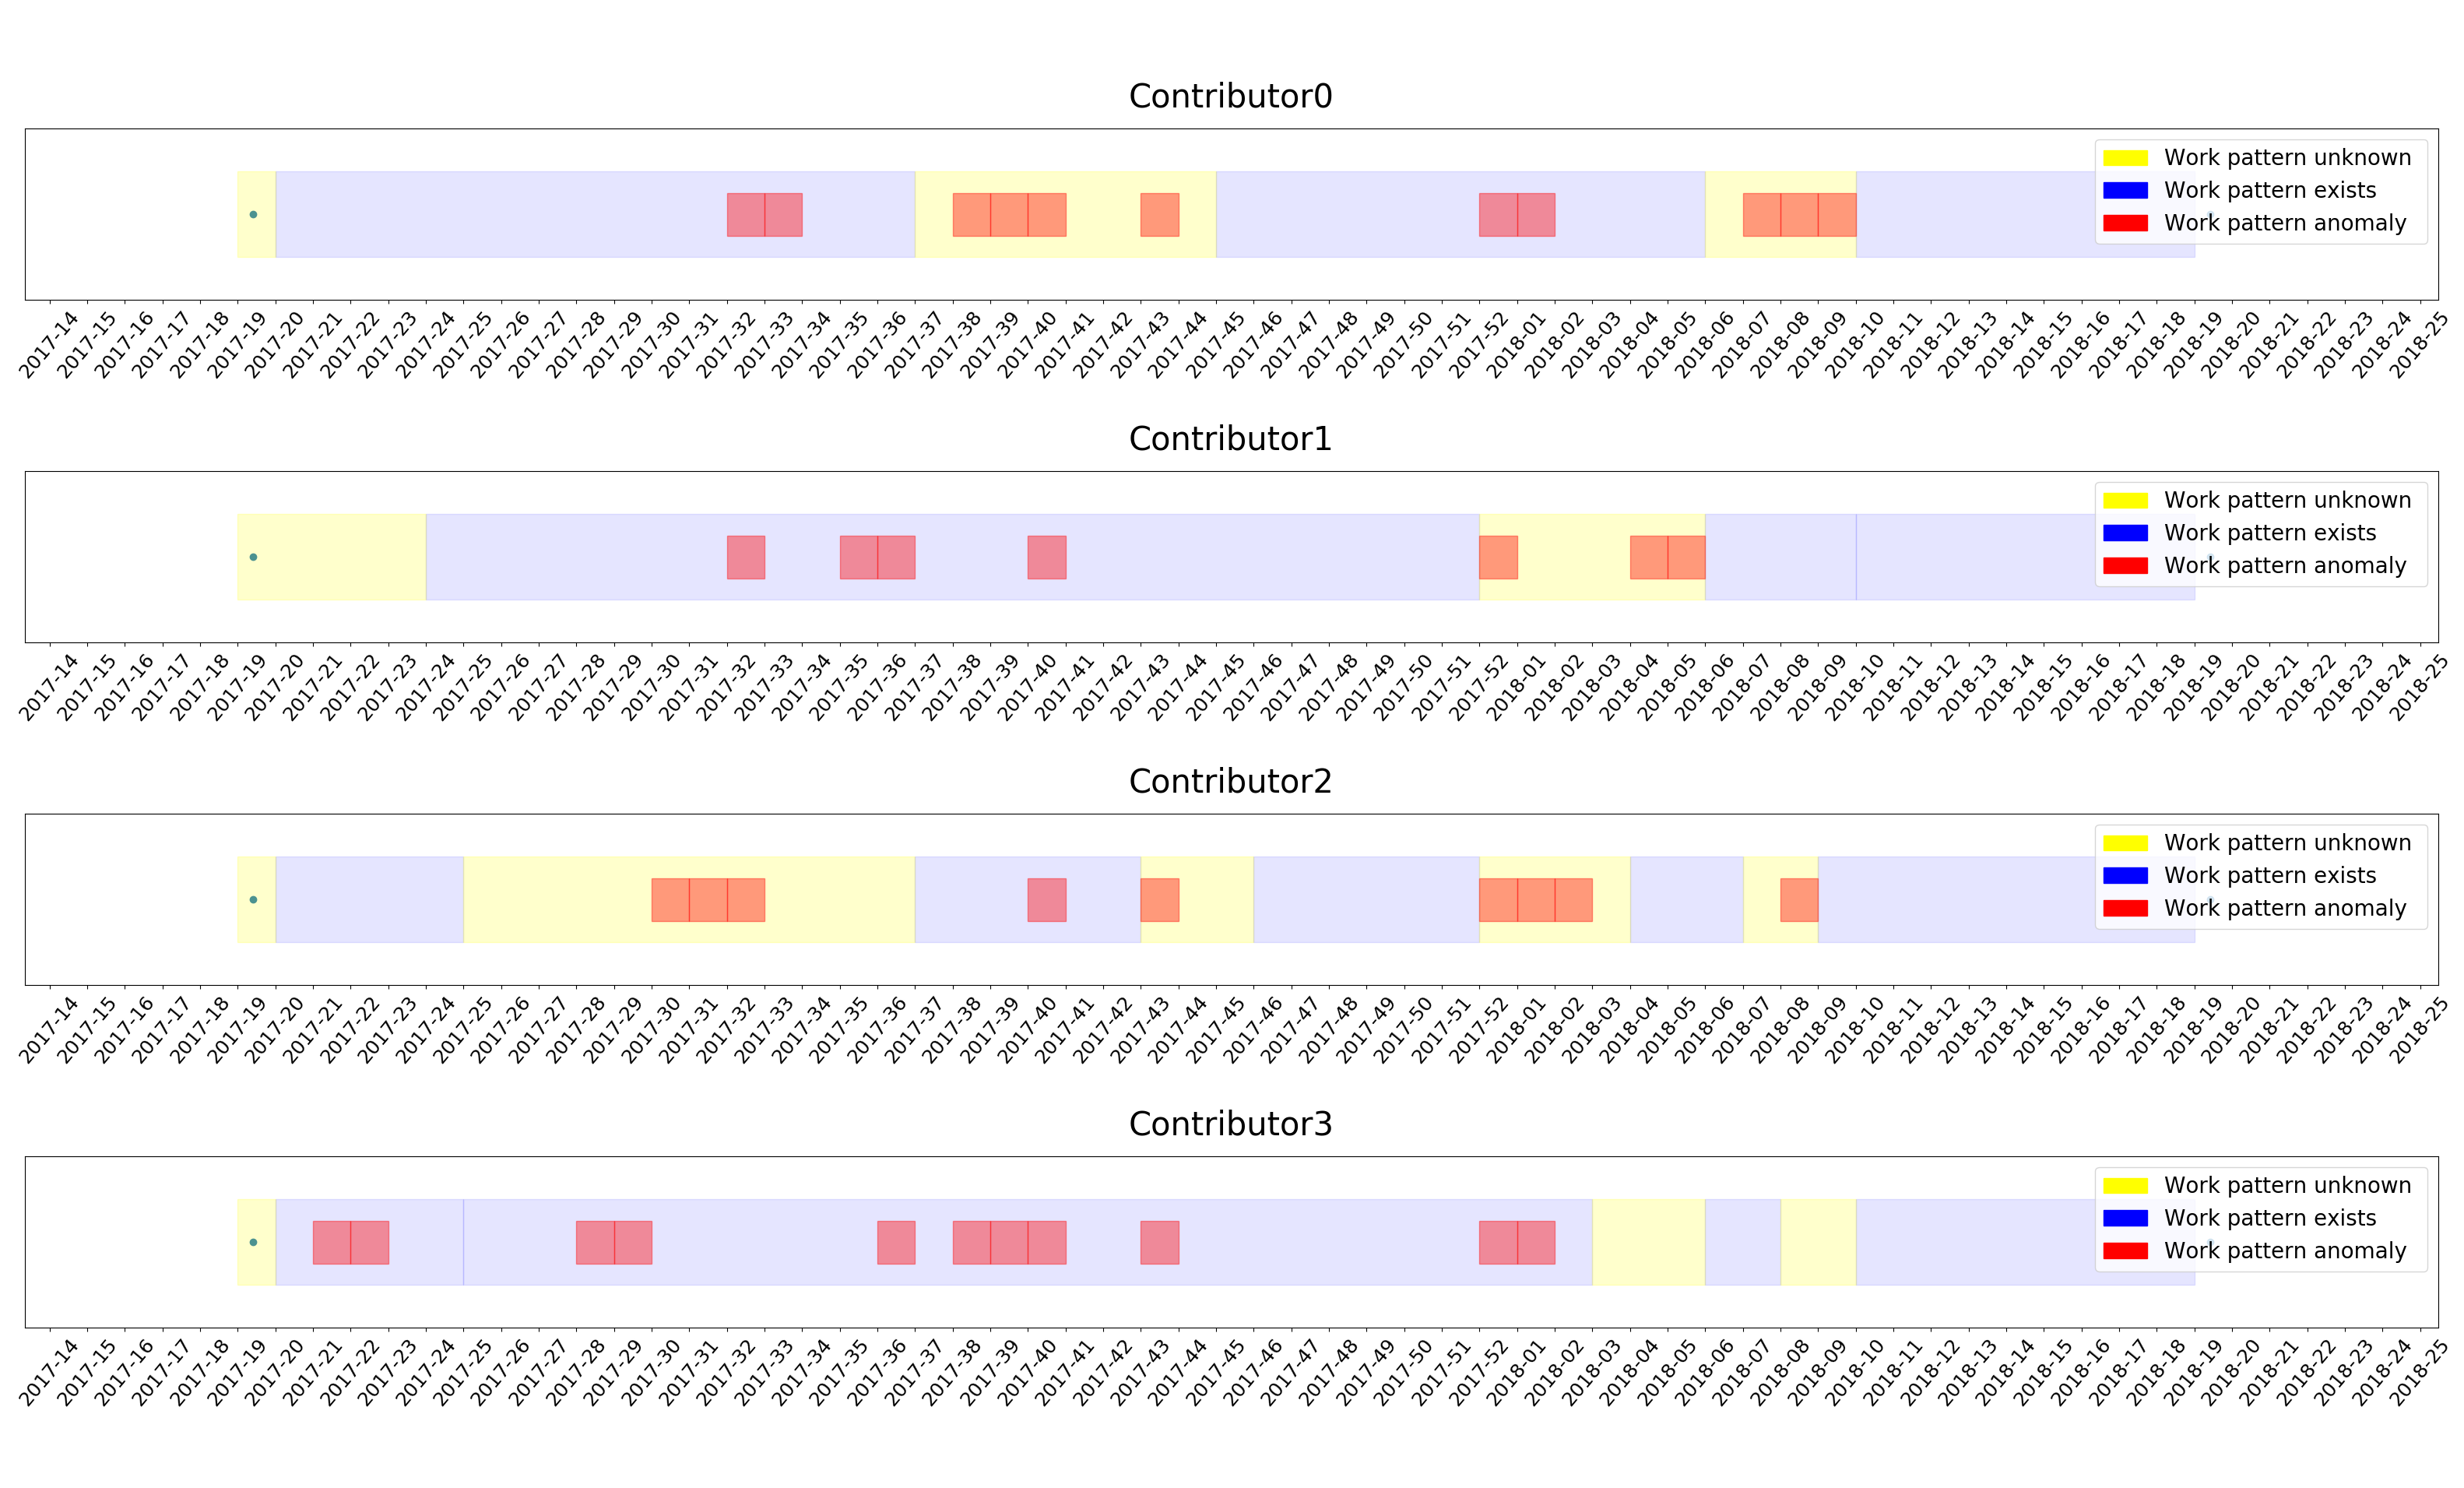
\includegraphics[scale=0.19]{./graphs/analysis/work-time-analysis-comparison}
    \centering
    \caption{The miss-out analysis graphs of the four employees from the survey.}\label{fig:miss-out-comparison}
\end{figure}

In Figure~\ref{fig:miss-out-comparison} the comparison between multiple employees can be seen.
\emph{Contributor0} and \emph{Contributor2} are working on flexible work time, which reflects in the inconsistencies in the work patterns (yellow sections in Figure~\ref{fig:miss-out-comparison}) of those contributors.
The other two contributors have very consistent working hours patterns, as can be seen by the long-lasting blue sections.


\section{Sleep Rhythm and Working Hours}

\subsection{Sleep Rythm}
To evaluate the significance of the punch card in terms of sleep rhythm analysis, a small survey in a closed community has been made.
A group of ten people, who know each other well, has been selected for this purpose.
Furthermore, a subset of four people has been chosen who were going to be evaluated.
The data gathered for the test group only contained their leisure time contributions, as their work repositories were not open-source.
All ten people then needed to assign the punch card of those four persons to a specific person.
The specific task given to test group was to assign each punch card to a specific person based on their knowledge about their sleep rhythm and leisure time behavior.

To this end, three quite similar patterns, from which one contributor has a very regular sleep rhythm (Subfigure 2 in Figure~\ref{fig:punchcard-survey}) and one pattern of a practically inexistent sleep rhythm (Subfigure 1 in Figure~\ref{fig:punchcard-survey}) have been selected.

For the three similar graphs, no significant results could be assessed, as the assignments were more or less random.
The contributor with the irregular sleep rhythm, on the other hand, got correctly assigned in all cases.

Sadly, as such a survey needs very specific targeting and a long lead time for data collection, it could only be executed on a small number of subjects.
Anyhow the result of this survey indicates that there exists a correlation between the structure of the punch card and the sleep and leisure time commit behavior of a contributor, even if it can only be accurately assigned in extreme cases.


\begin{figure}[H]
    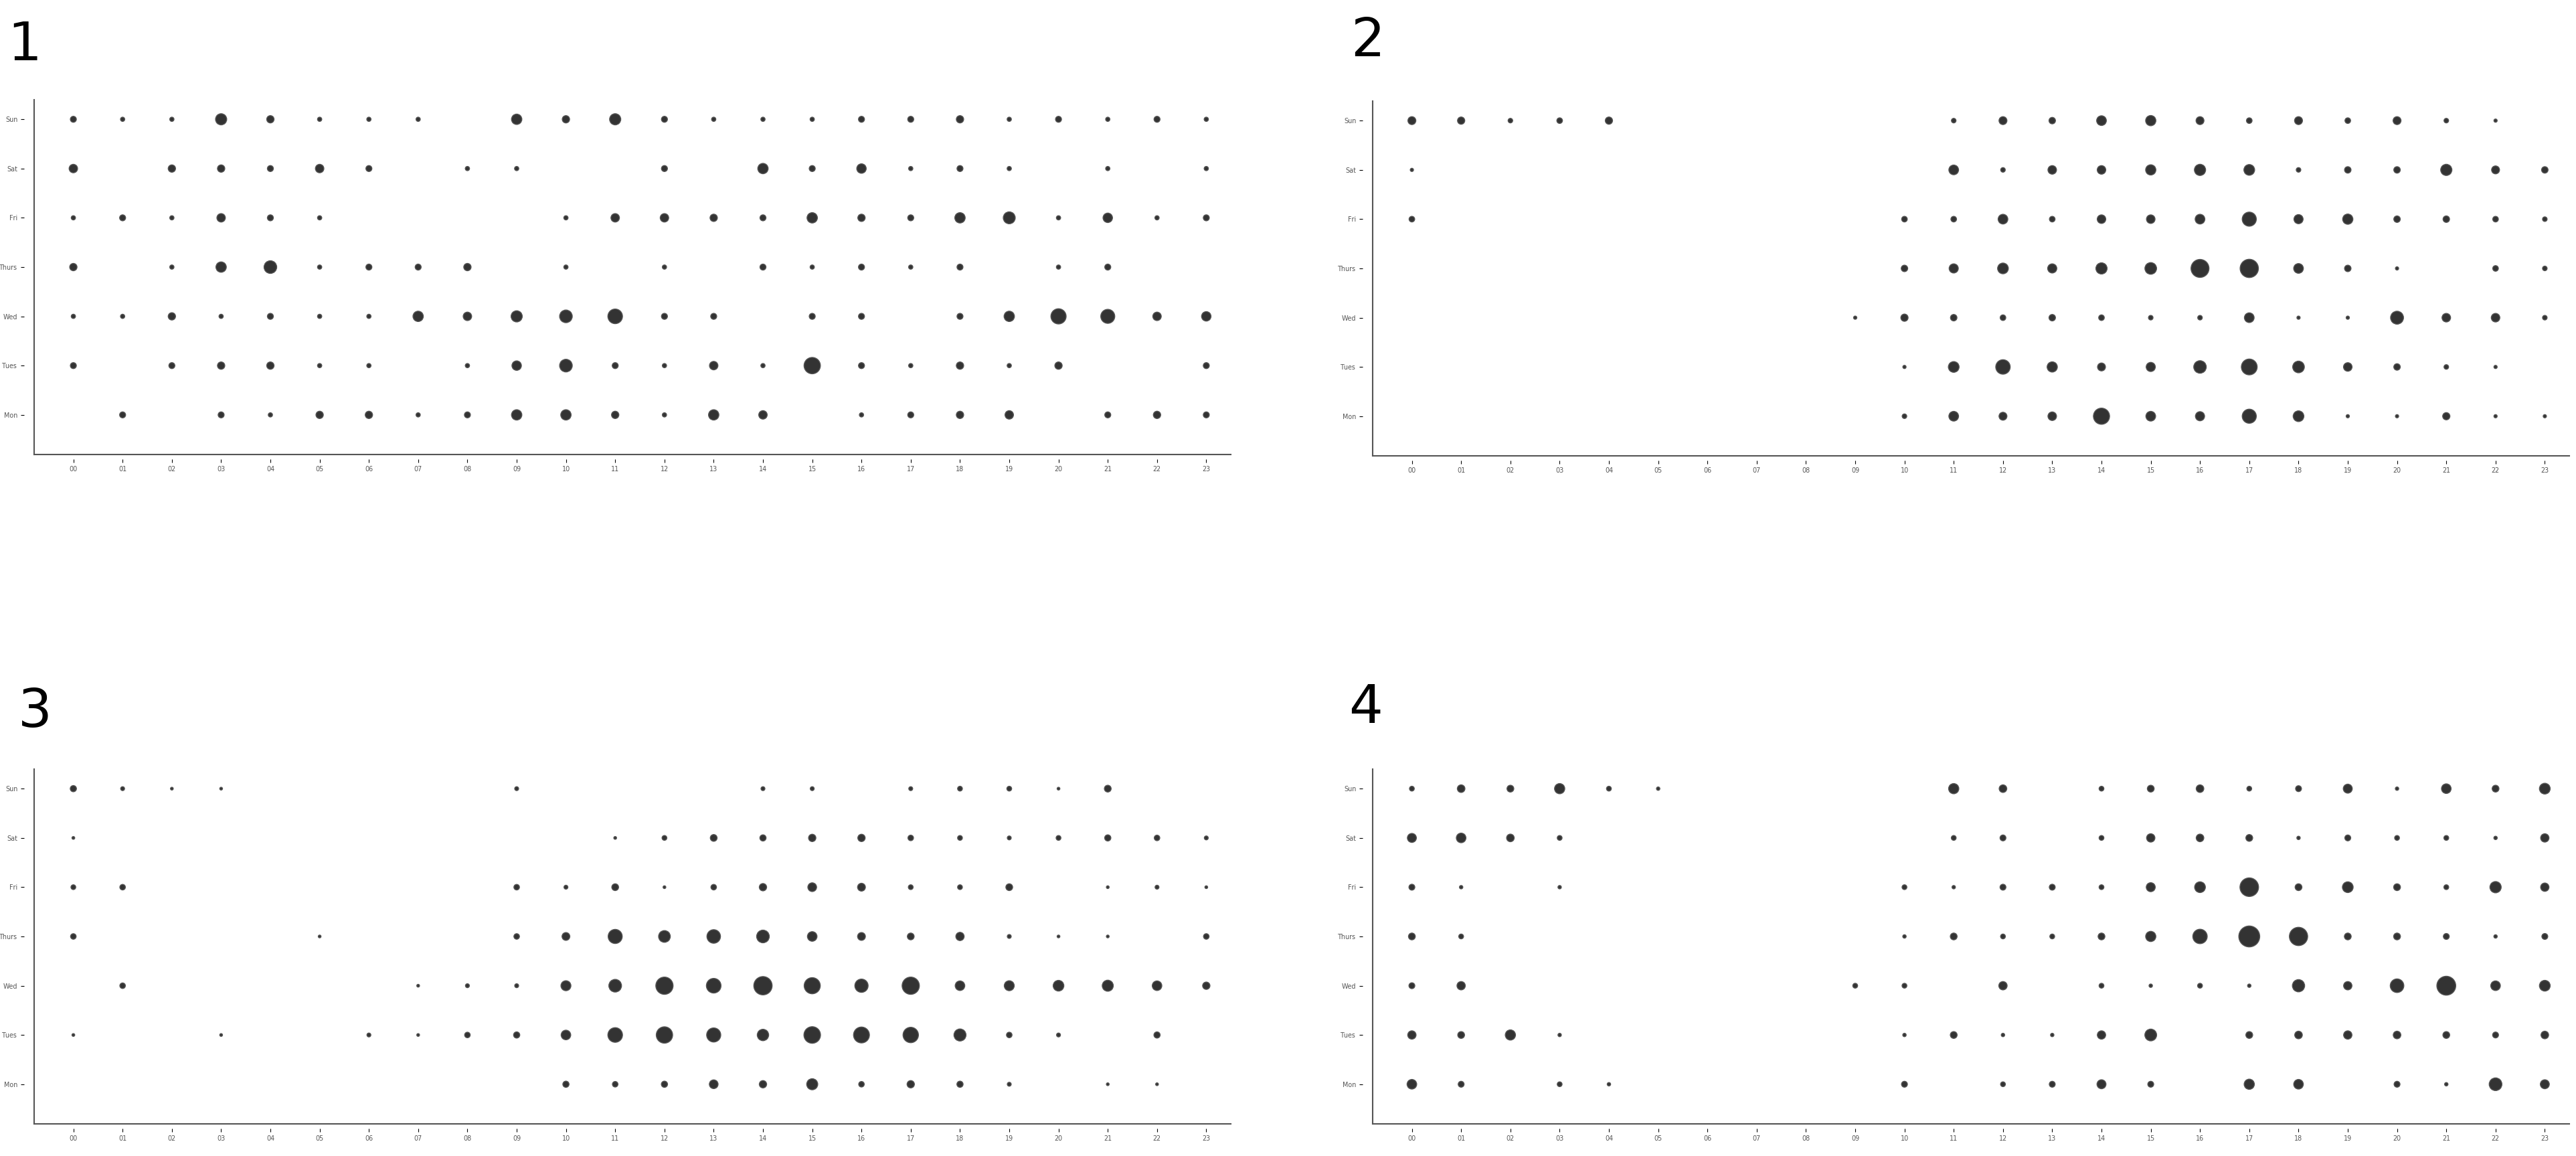
\includegraphics[scale=0.16]{./graphs/analysis/survey_combined}
    \centering
    \caption{The punch cards created and used for the test group in the survey.}\label{fig:punchcard-survey}
\end{figure}

\subsection{Employee or Open-Source Contributor}
To determine whether a punch card could be used to distinguish between an employee or an open-source volunteer, the results of the clustering described in Section~\ref{punchcard-implementation} have been utilized.
For this approach, two assumptions have been made.
A usual employee works between Monday and Friday during the day and only as an exception at the weekend, an example cluster can be seen in Figure~\ref{fig:normal-office-hours}.
An open-source volunteer works outside of the usual work shifts, which means early and late during weekdays and at the weekend, an example cluster can be seen in Figure~\ref{fig:leisure-time-hours}.

\begin{figure}[H]
    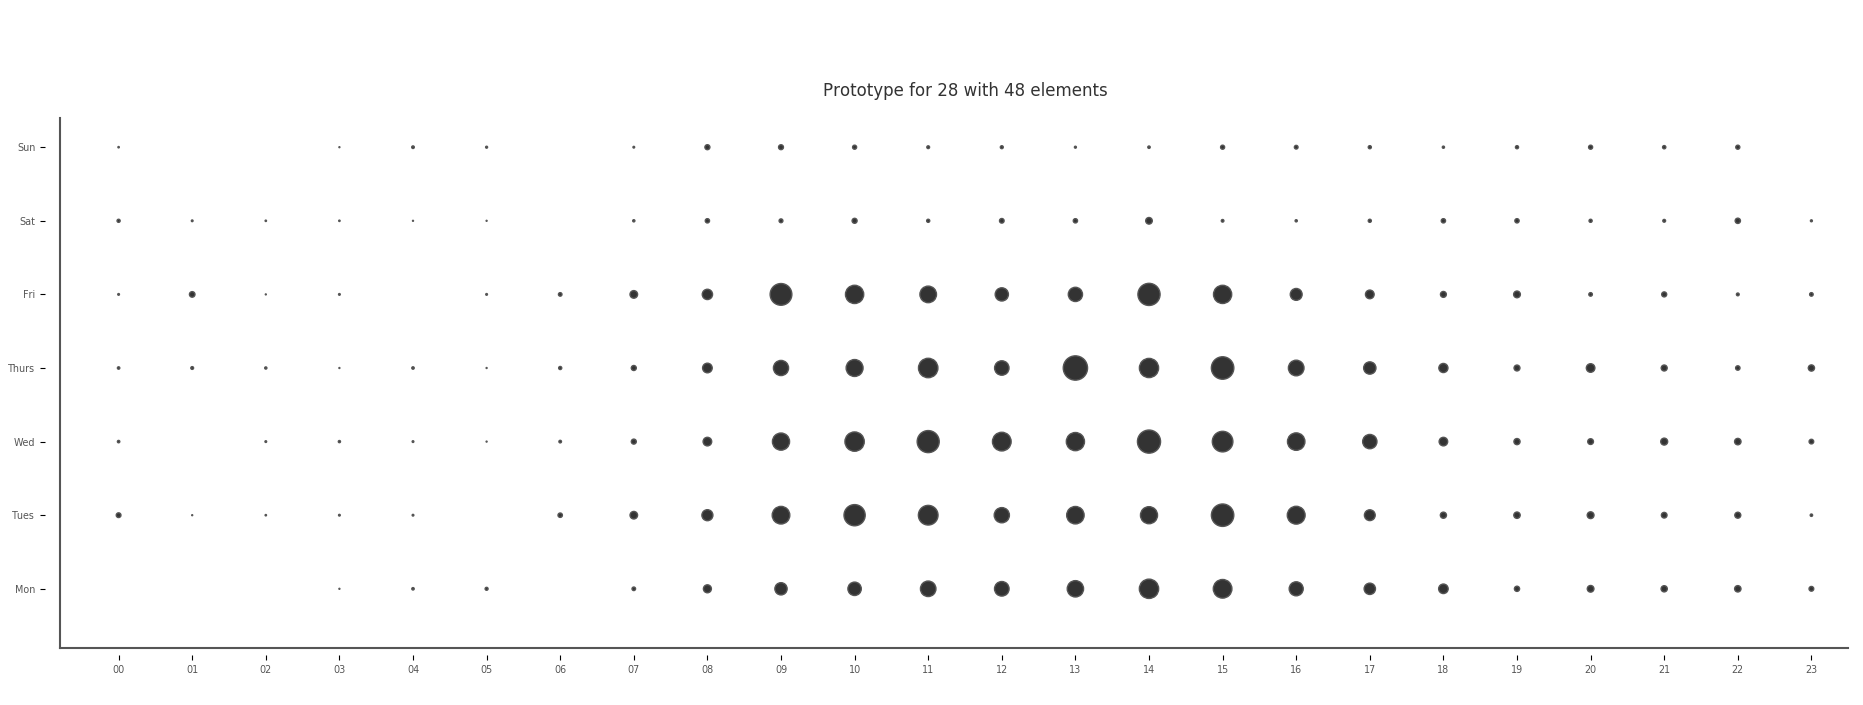
\includegraphics[scale=0.32]{./graphs/analysis-affinity/28}
    \centering
    \caption{Punch card of an example from an affinity propagation cluster of contributors with normal work shifts.
    A clear tendency to regular office working hours can be seen (Monday to Friday between 7:00 and 18:00 o'clock)}\label{fig:normal-office-hours}
\end{figure}

For each assumption, two representative clusters have been chosen and ten random persons have been selected from each cluster.
The manual verification is conducted by checking if the contributor mainly contributes to repositories which belong to the registered employee.
If no employee is registered, but other sources such as a homepage are provided, the information of these sources is checked for possible employee details as well.
In case no employee exists, it is examined whether the contributor pushes to their own and to open-source projects or rather to the repositories of a specific company.

\begin{figure}[H]
    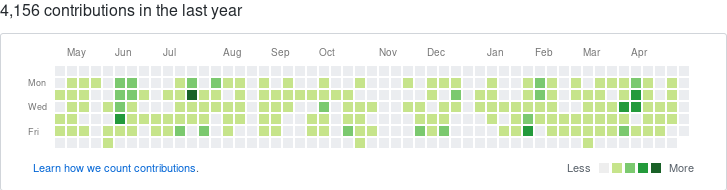
\includegraphics[scale=0.6]{./graphs/contribution-overview-alxhub}
    \centering
    \caption{Github contribution overview of a Google developer with the nickname alxhub.}\label{fig:github-contribution-overview}
\end{figure}

For this purpose, the Github contribution overview on the contributors' profile page has been used.
An example of such an overview can be seen in Figure~\ref{fig:github-contribution-overview}.
It provides a good overview of the usual weekday work pattern over the last year and allows to quickly inspect the repositories a contributor committed to at a specific month.

\begin{figure}[H]
    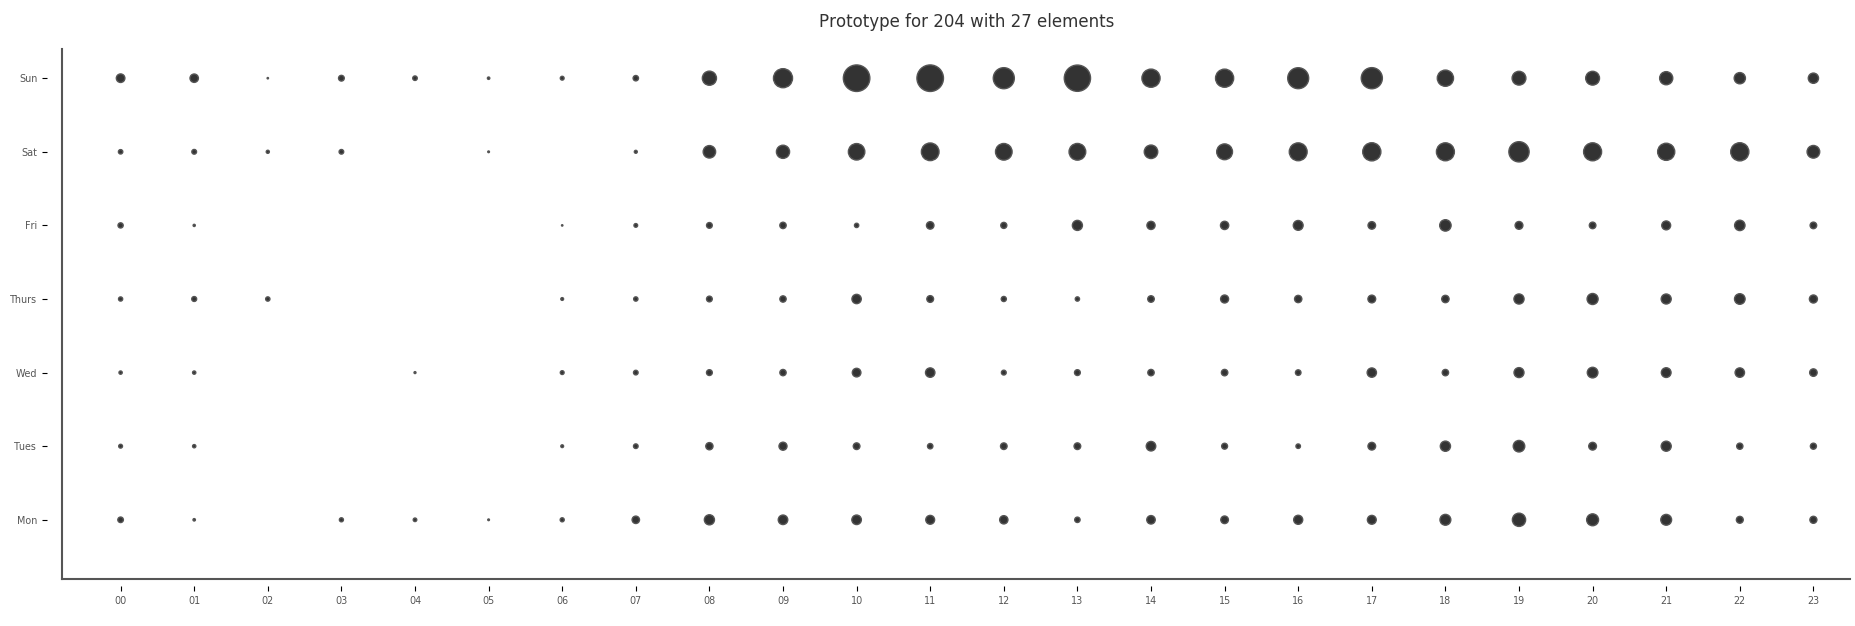
\includegraphics[scale=0.32]{./graphs/analysis-affinity/204}
    \centering
    \caption{Punch card of an example from an affinity propagation cluster of leisure time contributors. A clear tendency to contributions out of regular working hours and at the weekend.}\label{fig:leisure-time-hours}
\end{figure}

The representatives for the usual five-day week commit behavior were surprisingly accurate.
19 out of 20 considered contributors were mainly working on projects of their companies, with occasional commits to other open-source projects.
For the remaining contributor, it could not be determined if they work for a company.

The representatives for the leisure time commit behavior are mostly correct as well.
15 out of 20 considered contributors were irregularly contributing to either work unrelated open-source projects or to their own projects.
See Appendix~\ref{tbl:leasure-time-cluster-evaluation} for a table with the results of the leisure time cluster evaluation.
The remaining five contributors were either contributors working and committing to their employee's projects, but also to their own and open-source projects or employees with an untypical commit behavior.

This analysis shows quite well, that there is a correlation between the assumed patterns and the Github commit behavior or the usage of their Github accounts.
Unfortunately, the evaluation process for these results is very time consuming and thereby only a relatively small sample (n=40) has been chosen.
As it is not trivial to link the employee of a contributor to all their funded projects, all verification needed to be conducted manually.

\begin{landscape}
    \begin{table}[]
        \centering
        \captionof{table}{Employee cluster evaluation.}\label{tbl:employee-cluster-evaluation}
        \begin{tabular}{lllll}
            \toprule
            Nickname      & Employer     & Main projects                & Work related & Over 90\% work related \\
            \midrule
                          &              &                              &              &                        \\
            brettfo       & Microsoft    & visualfsharp                 & yes          & no                     \\
            aputinski     & Salesforce   & Salesforce                   & yes          & yes                    \\
            alxhub        & Google       & Angular                      & yes          & yes                    \\
            MatrixFrog    & Google       & Google Projects              & yes          & yes                    \\
            ryanemerson   & Red Hat      & Infinispan                   & yes          & no                     \\
            garagatyi     & Red Hat      & Eclipse and related projects & yes          & yes                    \\
            eternoendless & PrestaShop   & PrestaShop                   & yes          & yes                    \\
            initvector    & vanilla      & vanilla                      & yes          & yes                    \\
            kyhavlov      & HashiCorp    & HashiCorp                    & yes          & no                     \\
            XenoPhex      & CloudFoundry & CloudFoundry                 & yes          & yes                    \\
            gjoranv       & unknown      & vespa-engine/vespa           & probably     & yes                    \\
            doolse        & Equella      & Equella                      & yes          & yes                    \\
            leplatrem     & Mozilla      & Mozilla/Kinto                & yes          & yes                    \\
            StrongMonkey  & Rancher Labs & Rancher Labs                 & yes          & no                     \\
            lukaseder     & jOOQ         & jOOQ                         & yes          & yes                    \\
            DaazKu        & vanilla      & vanilla                      & yes          & yes                    \\
            brettcannon   & Microsoft    & Microsoft/Python             & yes          & yes                    \\
            isidorn       & Microsoft    & Microsoft Projects           & yes          & yes                    \\
            jackhorton    & Microsoft    & Microsoft Projects           & yes          & yes                    \\
            glasserc      & Mozilla      & Mozilla/Kinto                & yes          & yes                    \\
            nickwei84     & CloudFoundry & CloudFoundry                 & yes          & yes                    \\
            \bottomrule
        \end{tabular}
    \end{table}
\end{landscape}


\subsection{Bot Detection}
Another possible attack that opened up during the creation of the clusters was the detection of automatically committing programs, so-called \emph{bots}.
Several clusters showed a very consistent commit behavior around a specific hour, such a punch card can be seen in Figure~\ref{fig:bot-punchcard}.

\begin{figure}[H]
    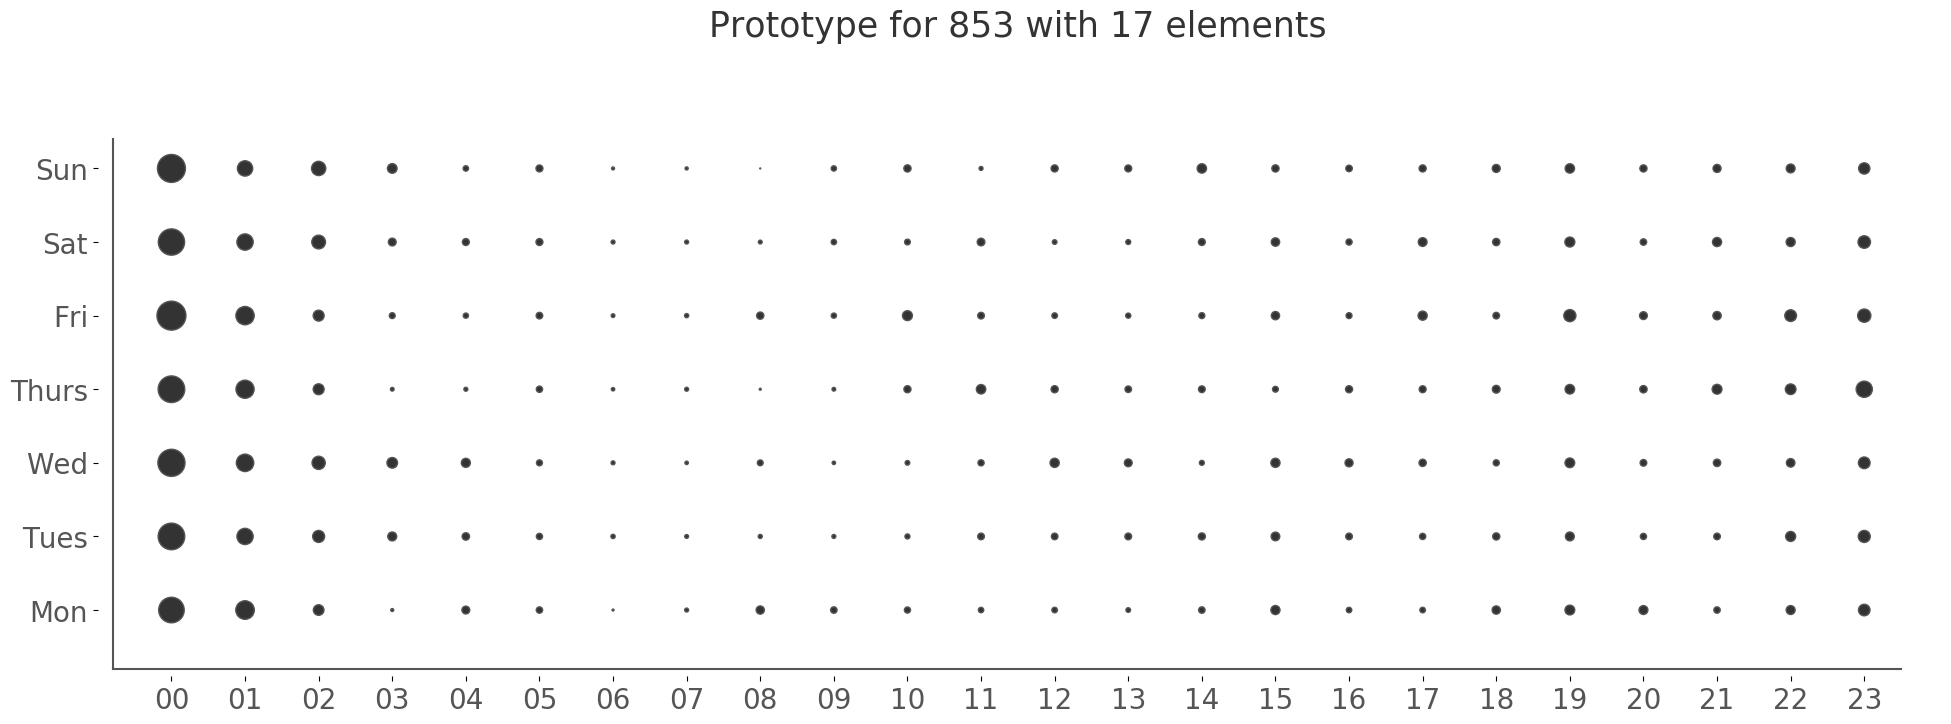
\includegraphics[scale=0.32]{./graphs/analysis/bot-punchcard}
    \centering
    \caption{A punch card with an extraordinary commit pattern around midnight. This might indicate a regularly automatically committing program, a so-called \emph{bot}}\label{fig:bot-punchcard}
\end{figure}

In the following, I implemented an algorithm which simply detected centroids with an extremely equally distributed pattern or patterns with a spike at a specific hour.
After a manual revision of the clusters detected by this methodology, it became apparent that only a very small subset of those clusters actually contained bots.
Even if the cluster contained bots there usually were only one or two of a much larger pool of cluster members.

Detection of bots in the outliers, which were not assigned to any cluster, did not seem to be promising as well.
Manual revision of over 100 possible candidates led to not a single bot.
After reviewing these results, I decided that there is currently no viable approach to this problem.


\subsection{Fingerprinting}
Another possible attack was to fingerprint a contributor and create a unique identifier by analyzing their commit behavior.

This attack soon proved to be unfeasible, as the pattern of a contributor can significantly differ from month to month, as can be seen in Figure~\ref{fig:october-punchcard} and Figure~\ref{fig:november-punchcard}.

\begin{figure}[H]
    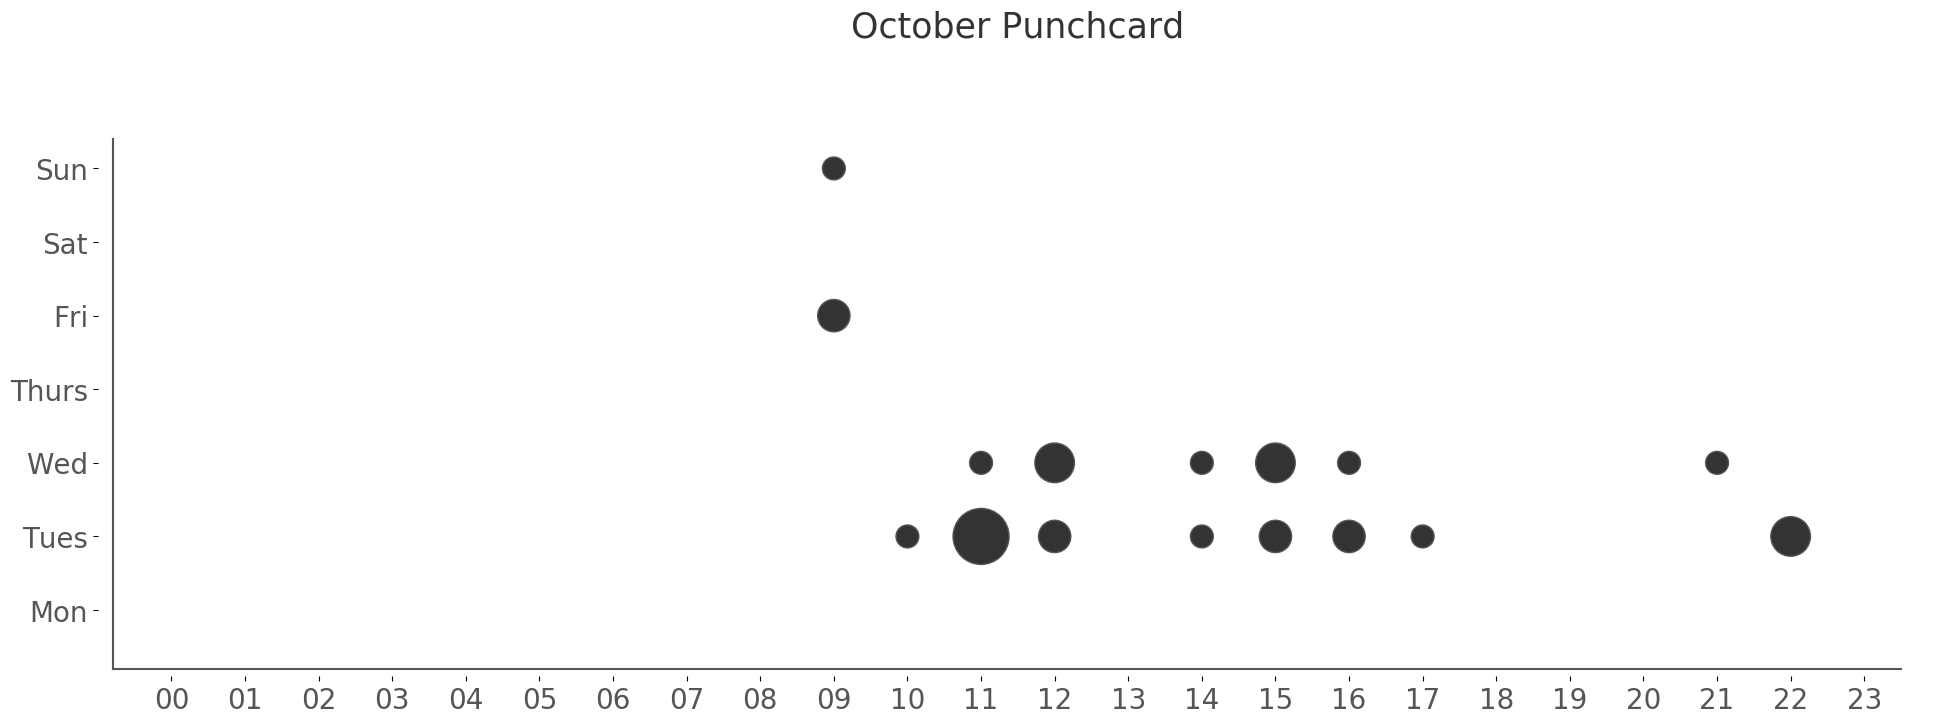
\includegraphics[scale=0.32]{./graphs/analysis/october-punchcard}
    \centering
    \caption{The author's punch card from October 2017.}\label{fig:october-punchcard}
\end{figure}

\begin{figure}[H]
    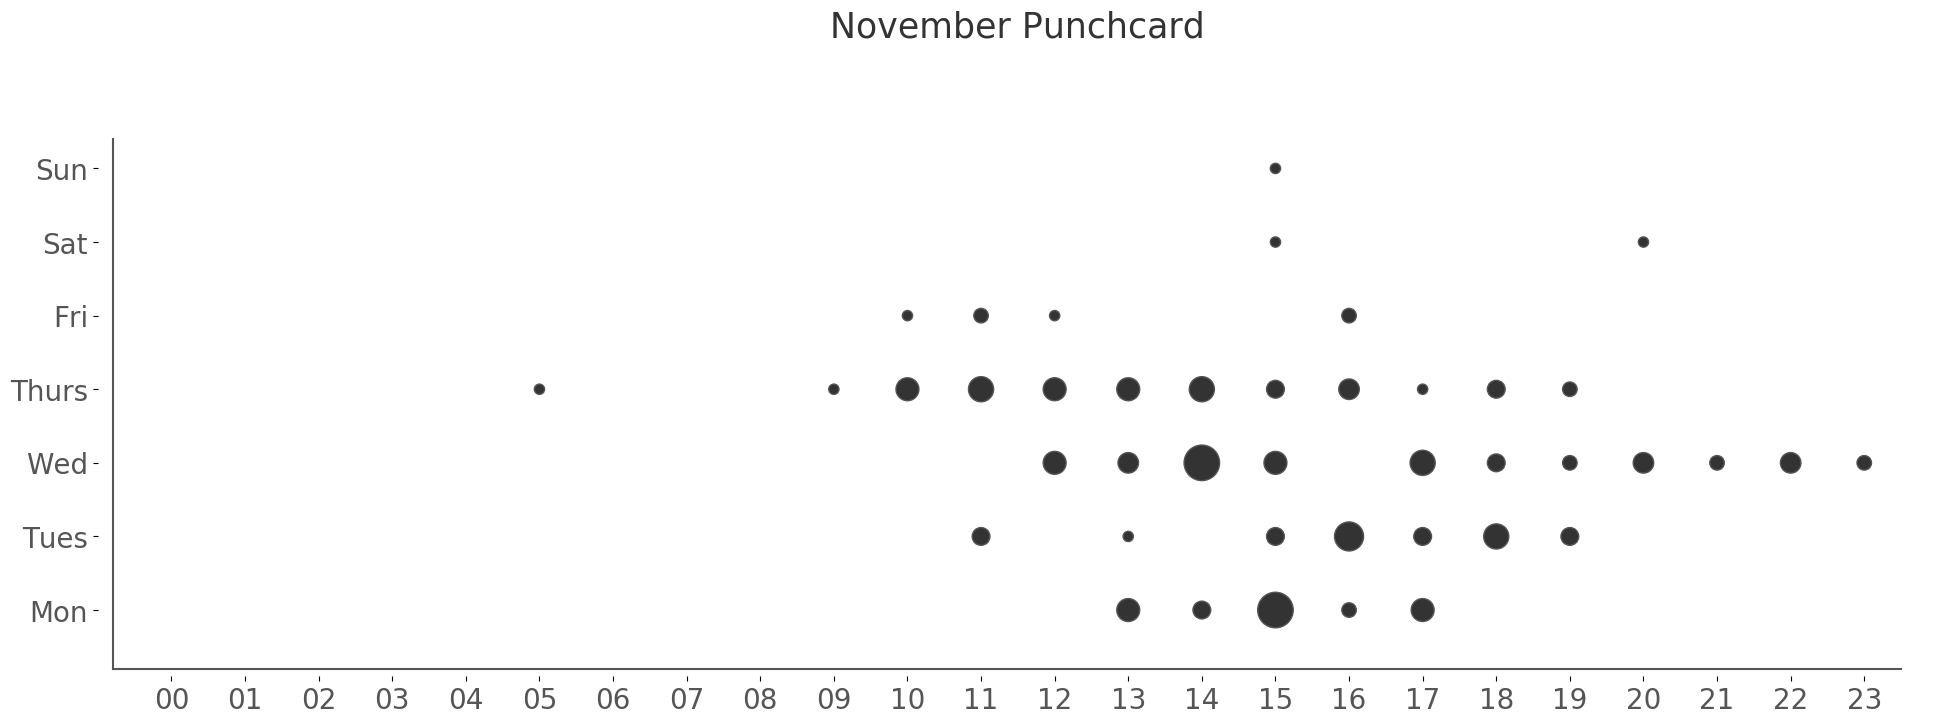
\includegraphics[scale=0.32]{./graphs/analysis/november-punchcard}
    \centering
    \caption{The author's punch card from November 2017.}\label{fig:november-punchcard}
\end{figure}

If the interval of a year is considered and the compared interval is shifted by a single month, the occurring changes are not that drastic, but still too different to see a consistent pattern over a longer time.
The commit behavior of people seems to be too inconsistent to create a unique fingerprint.


\clearpage
\section{Geographic Location}

First of all, it needs to be clarified that parts of this attack only works under specific circumstances.
Git commit timestamps are created by taking the current local time of the underlying \ac{os}.
If one wants to show the travel path of a target, the target's \ac{os} needs to automatically adjust the \ac{utc} offset accordingly to the current geographic location of the device.

This feature is available for newer versions of popular \acp{os}, such as \emph{Windows}~\footnote{Ivan Jenic, `Your Time Zone Can Now Switch Automatically in Windows 10', windowsreport.com, https://windowsreport.com/time-zone-automatic-switch-windows-10 (accessed, 24.04.2018)}
and \emph{Mac Os}, but they are not enabled by default.
It is also available for Linux, for instance, with the \emph{tzupdate} package~\footnote{`Set the system timezone based on IP geolocation', github.com, https://github.com/cdown/tzupdate (accessed, 24.04.2018)}, but it needs to be manually installed and activated.

\begin{figure}[H]
    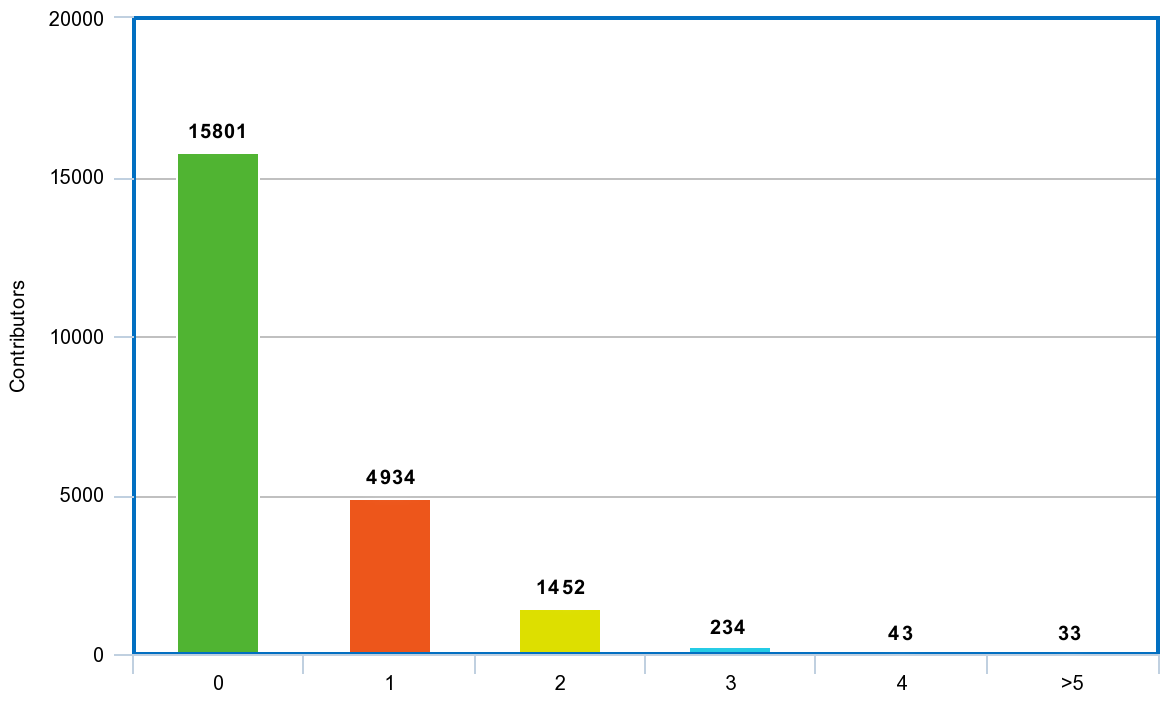
\includegraphics[scale=0.38]{./graphs/analysis/timezone-switch-distribution}
    \centering
    \caption{Distribution of users according to the amount of timezone switches detected by the algorithm.
    The major part of all contributors does not have any detectable timezone changes.}\label{fig:timezone-switch-distribution}
\end{figure}

Figure~\ref{fig:timezone-switch-distribution} shows the number of contributors in relation to the number of detected timezone switches.
On about 70\% of considered contributors, only a single timezone has been detected, looking at the last year.
These 70\% do either not commit when they travel, their \acp{os} do not synchronize the timezone accordingly to their location or they simply did not travel in the last two years.

\begin{figure}[h]
    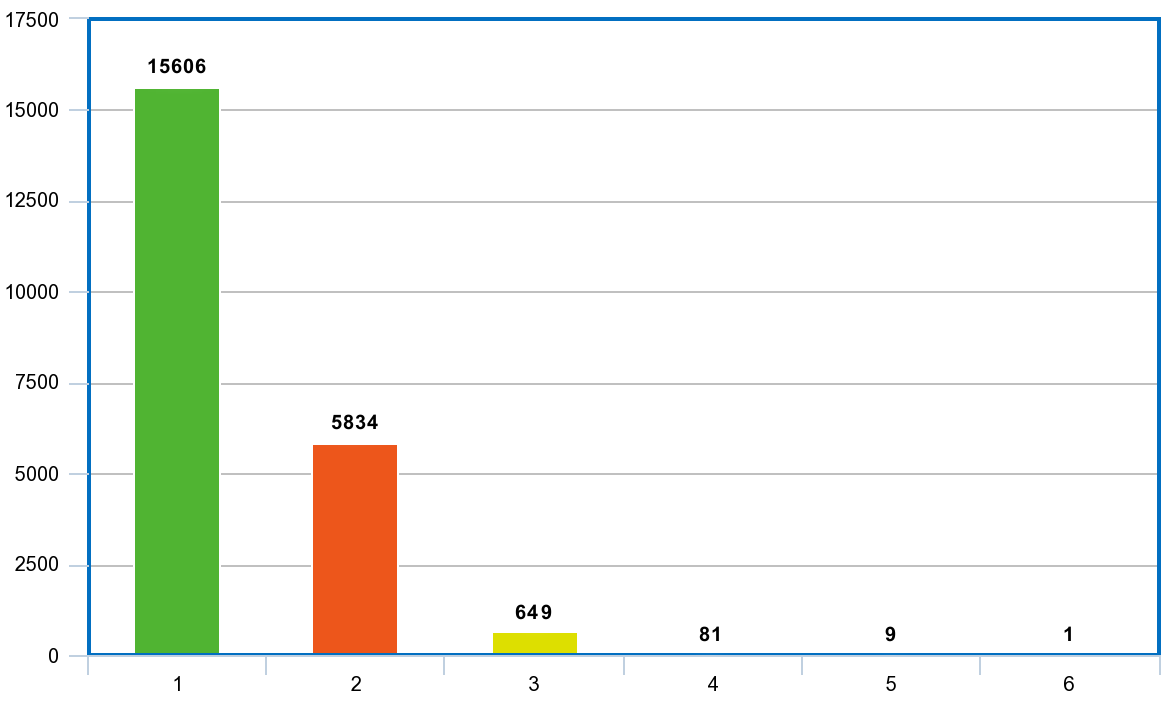
\includegraphics[scale=0.38]{./graphs/analysis/timezone-distribution}
    \centering
    \caption{Distribution of users according to the amount of the different timezones detected by the algorithm.}\label{fig:timezone-distribution}
\end{figure}

In Figure~\ref{fig:author-home-location} the visualized home location analysis of the author can be seen.
Regions marked in dark green are regions in which the contributor is likely to live.
The light green region represents the timezone of the home location.
As you can see in Figure~\ref{fig:author-home-location} the country of French Guiana is also marked as a possible home location.
This problem occurs due to the several conversions between country names and codes, which were necessary as stated in Section~\ref{timezone-implementation}.
This misassignment only happens during the visualization process of the results and thereby does not affect the results of the analysis.

\begin{figure}[h]
    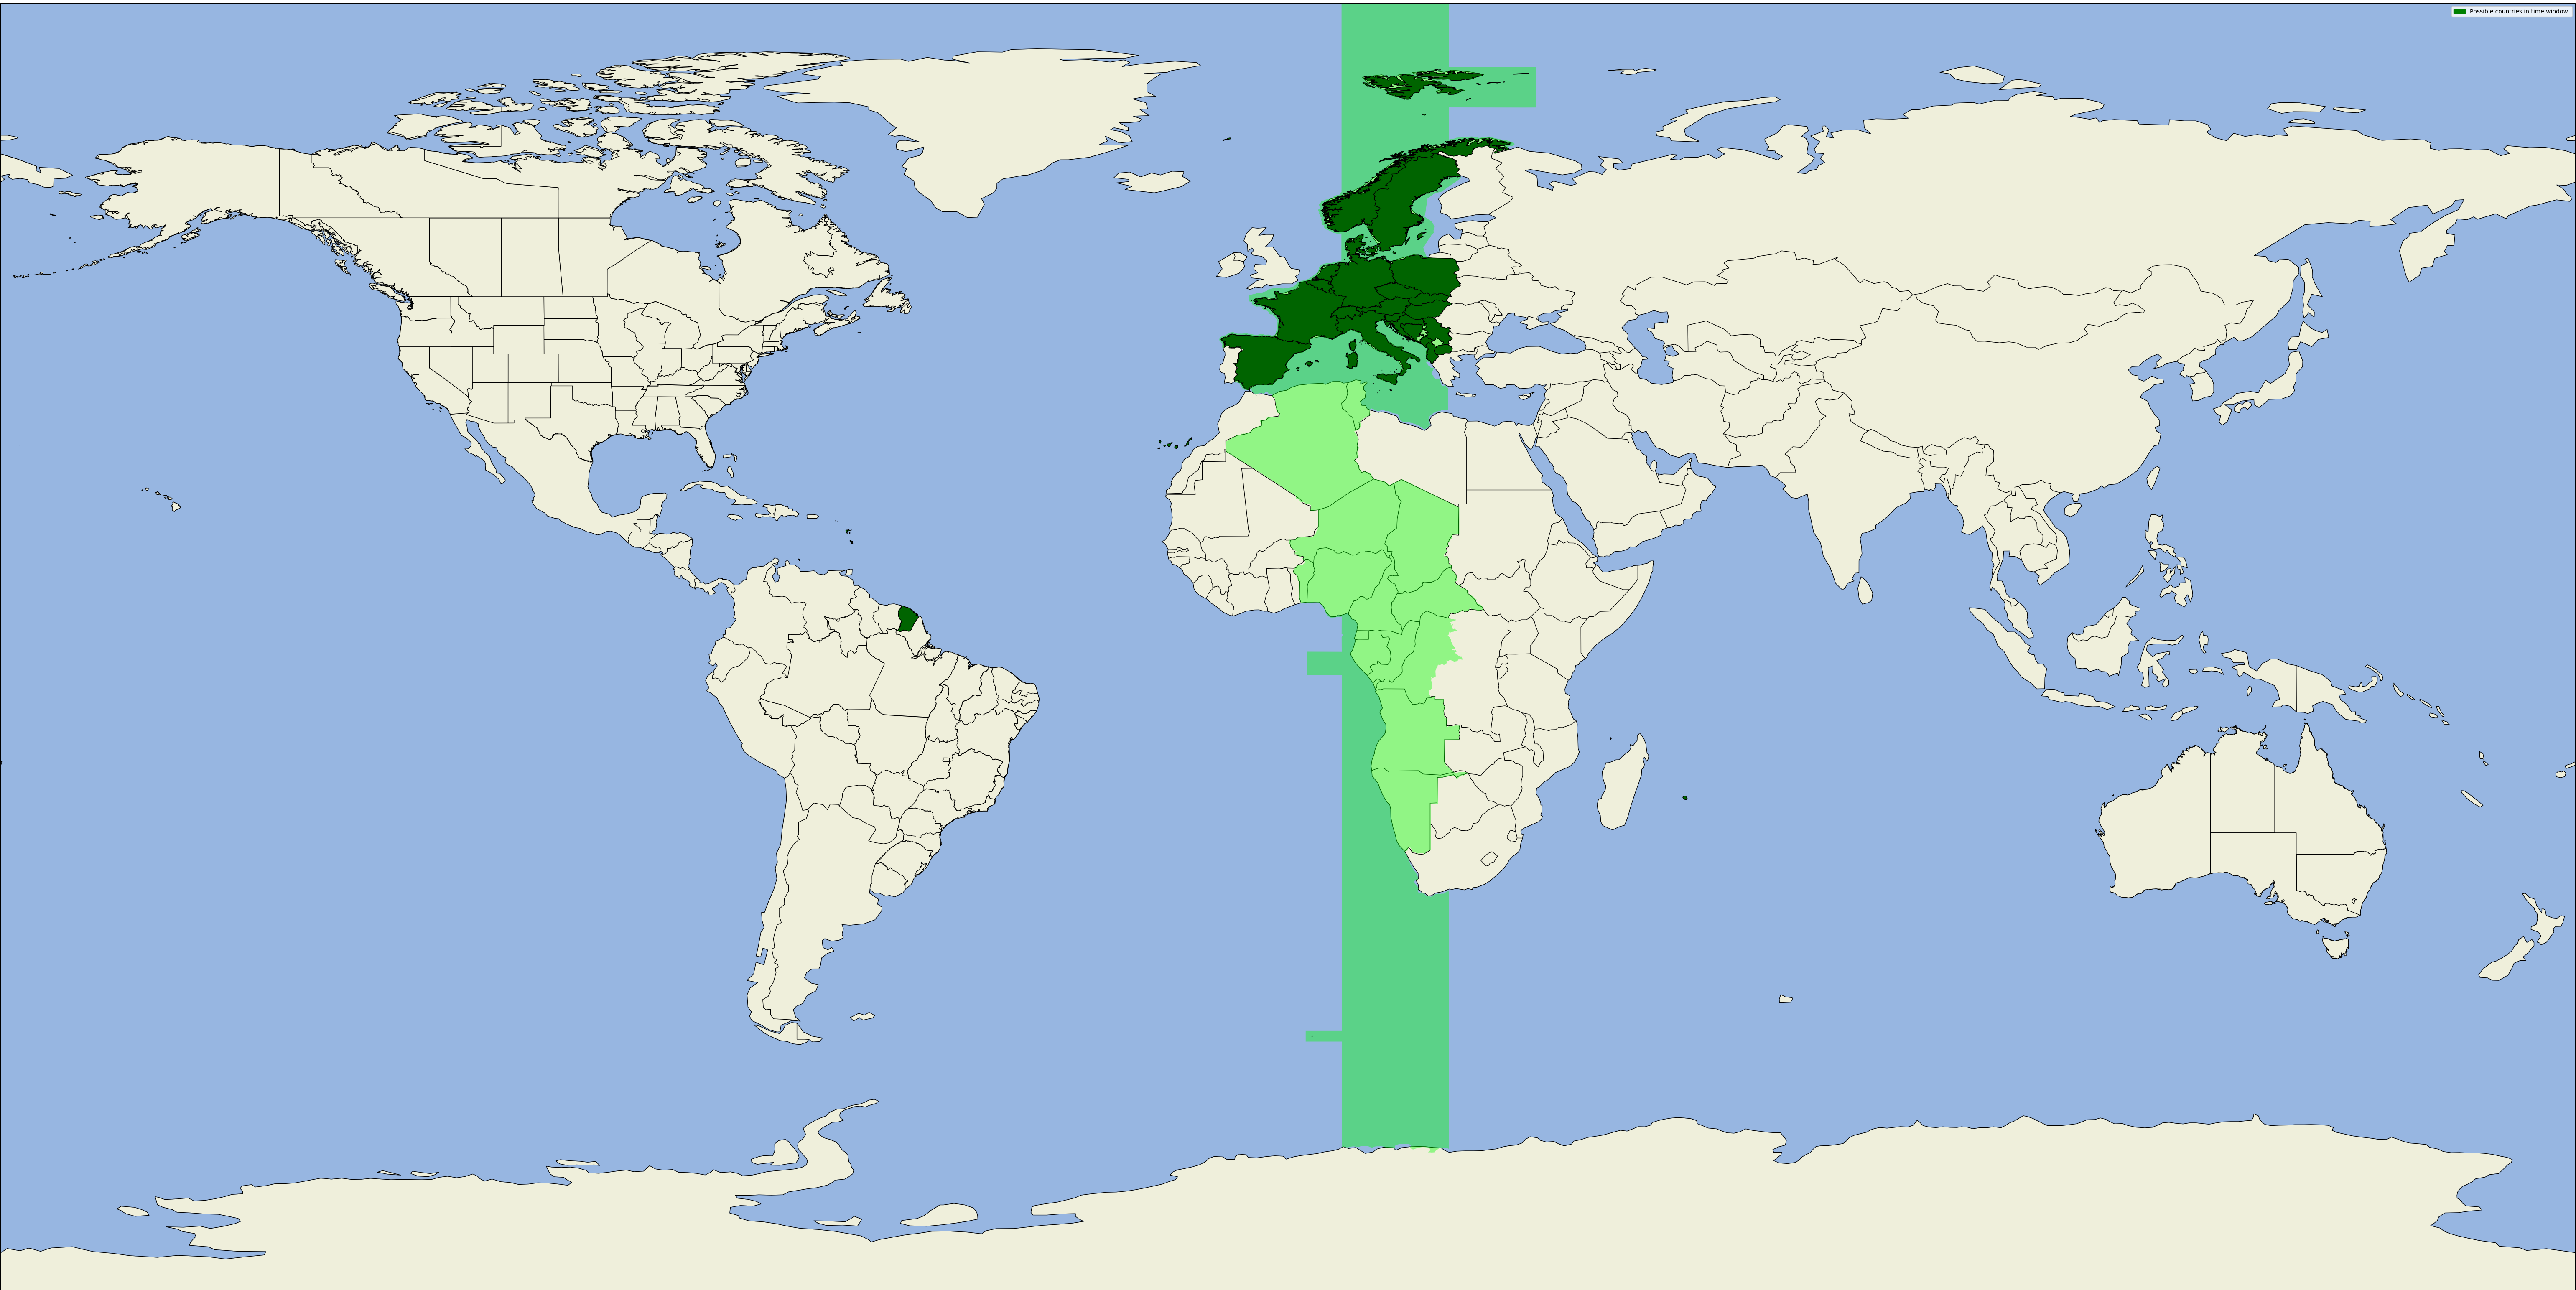
\includegraphics[scale=0.10]{./graphs/analysis/author-home-location}
    \centering
    \caption{The visualized home location analysis of the author.
    The light green indicates the timezone the target is probably in.
    The dark green color shows the remaining countries after considering \ac{dst} switches.}\label{fig:author-home-location}
\end{figure}

To evaluate the overall precision of the geographic location results, the correctness of the determined home locations are checked.
Github allows users to specify a string for their current home location, which is also collected during the data aggregation process.
Unfortunately, there are no conventions on how this string has to look like.
Initially, I tried to pass these strings to the OpenStreetMap \ac{api}, but this resulted in too many wrongly assigned locations.
The data provided by the users was obviously too arbitrary and full of mistakes for OpenStreetMap to handle.

As a result, I decided to manually choose a subset of locations by looking for distinct identifiers in the location strings.
For instance, every home location of a contributor, that contained \emph{Germany} or \emph{Deutschland} in their location string, should be in the timezone \inlinecode{Europe/Berlin}, which switches between \ac{cet} and \ac{cest}.
I created 14 such rules and was thus able to validate the home location of about 4200 contributors.
The assignment of the contributors home location was correct in about 82\% of the considered contributors.

It needs to be noted, that the accuracy of this result is quite certainly deteriorated by location strings which contain ambiguous information.
On manual review of the location strings there were strings such as \inlinecode{I love NYC} which belongs to a developer living in Germany.
The result might also be deteriorated by contributors who moved to another country in the last year, as we cannot detect those for sure.

It also needs to be noted, that the \ac{iana} database does not always have exact mappings for countries to their timezone.
For many countries or states, the current or an old capital city is used.
Some countries do not have an own timezone, such as Japan, which is included in \inlinecode{Pacific/Palau}.
The \ac{iana} database is the currently best viable approach, but for better results and a more fine-grained resolution, a specific mapping between countries, states and time zones would be necessary.

Nevertheless, an accuracy of 76\% clearly shows, that it is possible to narrow down the location of a contributor to a timezone and even to a subset of countries, see Table~\ref{home-location-table} for reference, by simply looking at their git commit timestamps.

\begin{landscape}
    \begin{table}[h]
        \centering
        \begin{tabular}{llrrrr}
            \toprule
            Query string & Expected timezone string & Considered & Correct & Timezone strings after DST & Before DST  \\
            \midrule
            & & & & & \\
            San Francisco        & US/Pacific           & 772        & 639     & 12.07   &  18     \\
            NYC, NY, New York    & America/New\_York    & 485        & 366     & 23.60   &  52     \\
            India                & Asia/Colombo         & 148        & 127     & 4       &  4      \\
            UK, United Kingdom   & Europe/London        & 667        & 510     & 13.14   &  22     \\
            France               & Europe/Paris         & 490        & 421     & 31.59   &  40     \\
            New Zealand          & Pacific/Auckland     & 59         & 52      & 4.76    &  9      \\
            Germany, Deutschland & Europe/Berlin        & 976        & 846     & 31.48   &  38     \\
            Poland               & Europe/Warsaw        & 180        & 154     & 31.56   &  40     \\
            Italy                & Europe/Rome          & 130        & 112     & 31.39   &  41     \\
            Tokyo                & Pacific/Palau        & 61         & 48      & 8.51    &  12     \\
            Spain                & Europe/Madrid        & 129        & 116     & 32.83   &  40     \\
            Los Angeles          & America/Los\_Angeles & 86         & 76      & 12.24   &  18     \\
            Adelaide             & Australia/Adelaide   & 2          & 2       & 4.00    &  4      \\
            Mexico               & Mexico/General       & 13         & 7       & 11.62   &  39     \\
            \bottomrule
        \end{tabular}
        \caption{Results of the home location evaluation.
        The first column shows the comma separated strings by which contributors are selected depending on their location.
        The second column is the timezone that is expected to be in the remaining home location timezone string set.
        }\label{home-location-table}
    \end{table}
\end{landscape}


\chapter{Evaluation and Interpretation}\label{evaluation}
In the previous chapter, the implementation of several possible attacks which could be performed on the gathered data has been shown.
This chapter will now attend to the evaluation of all results gained from these attacks.
I will present the extracted information from each algorithm and compare it to the real-world ground truth.
This information will be then be explained and audited in terms of precision and reliability.

\section{Holiday and Sick Leave Detection}

Figure~\ref{fig:missing-time} shows the analysis of an employee for their employer's repositories.
The y-axis represents the additions and deletions of commits, the x-axis represents the week of the respective year.
For better verification and evaluation of the results, a scatter plot with the additions and deletions of each commit has been added on top of individual miss-out graphs.

\begin{figure}[h]
    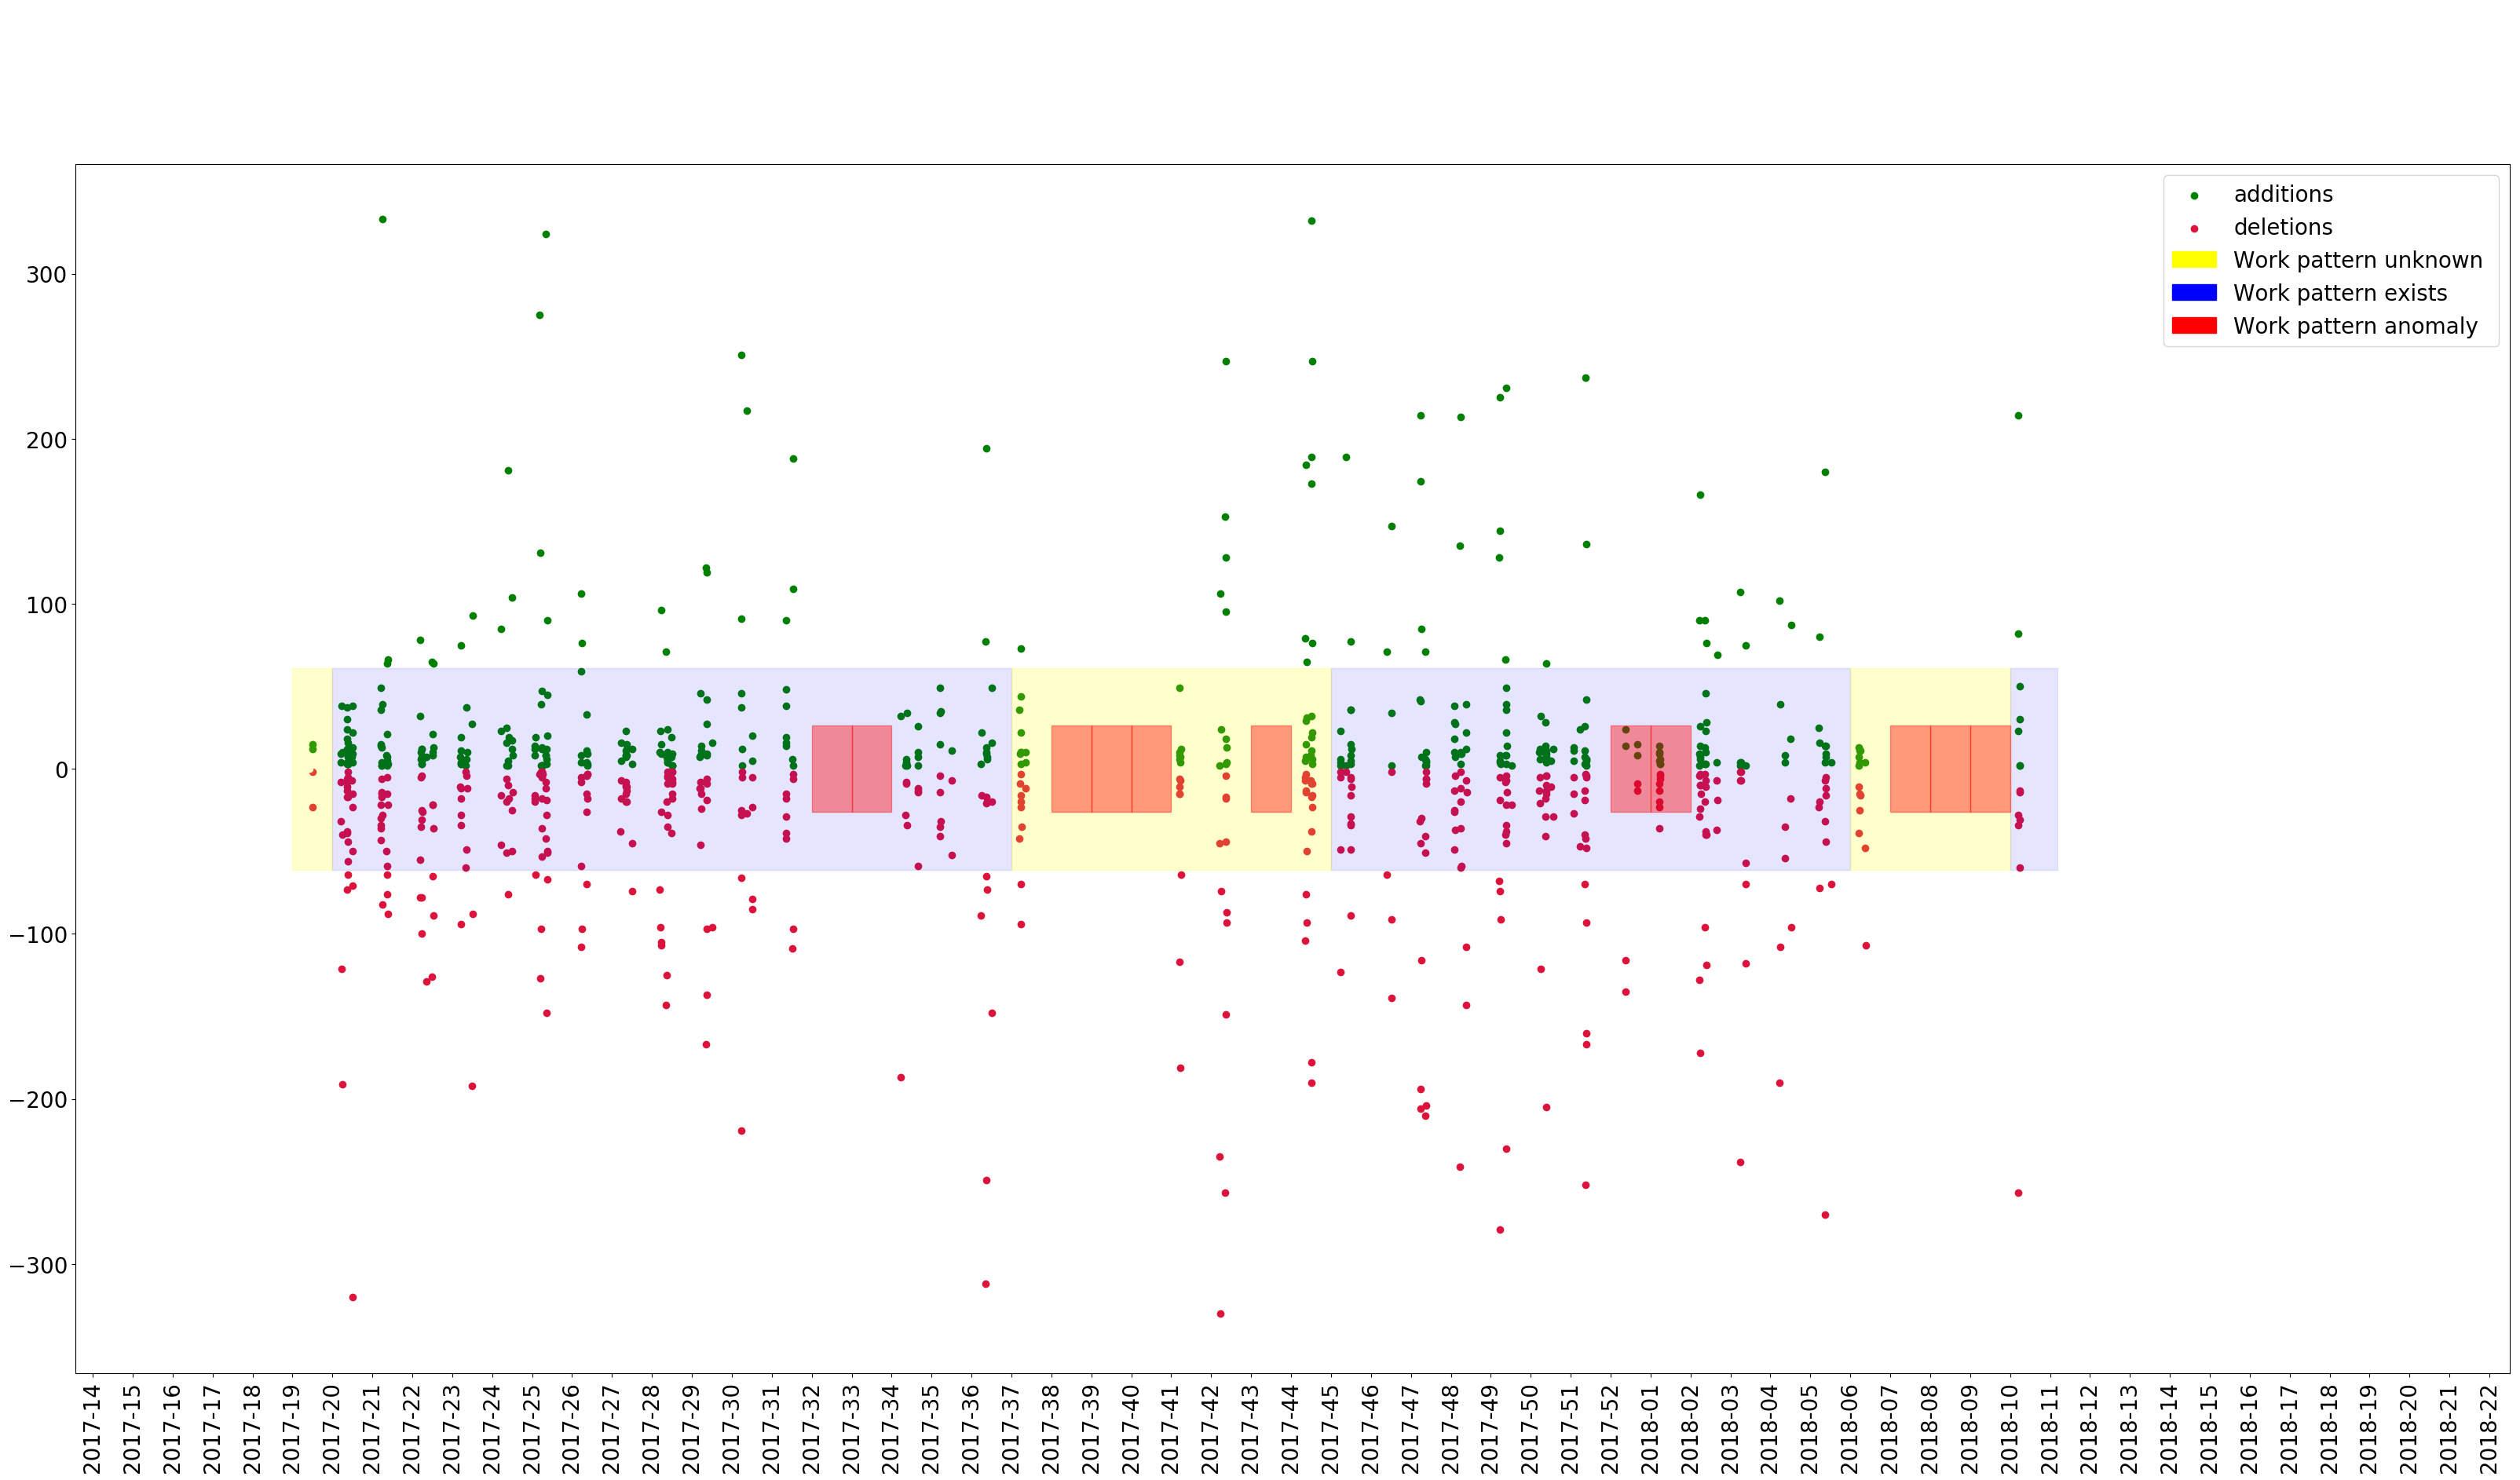
\includegraphics[scale=0.19]{./graphs/analysis/work-time-analysis}
    \centering
    \caption{
        The work time analysis of an employee.
        Blue sections are time spans in which the target has a consistent reoccurring week work pattern.
        Yellow sections show irregularities in their week work pattern.
        Red blocks are miss-out anomalies detected by the algorithm, which indicate holiday or sick leave.
    }\label{fig:missing-time}
\end{figure}

The evaluation of this algorithm turned out to be quite difficult, as there is no publicly available information about sick leave or holiday.
For the purpose of this thesis, I was allowed to use anonymous statistics of a company with a test group of five developing employees.

After scanning and analyzing the company's repositories, a survey has been conducted, for which each employee had to look at their visualized miss-out graph and check whether there are any wrong or missing detections.

The algorithm successfully managed to find all sick leave and holiday-related miss-outs in all cases.
However, there were three false positive cases.
Firstly a developer did work related research and did thereby not commit as regularly as usual, which was then detected as a miss-out.
Secondly, a developer contributed to repositories, which are not owned by the employee.
As a result, two weeks were marked as miss-out.
Thirdly there were two developers, that contributed to a branch, but their work has not been merged into the master branch yet, hence the commits were not being scanned yet.
This particular problem can be solved by not only scanning the master branch but also all other branches, however, this adds a lot of complexity to the continuous mining process and has thereby not been implemented yet.
Anyway, this problem only seems to occur in the latest weeks.

A not intended side effect of detecting prototypes is that the algorithm not only detected anomalies, such as sick leave or holiday, but also found inconsistencies in the work routine.
For instance between week 37 to 45 in Figure~\ref{fig:missing-time}, a developer was forced to reduce their working hours due to legal questions and continuously shifted hours and working days for several weeks.
It is hard to interpret those inconsistencies without more contextual information, but nevertheless, it provides the fact that something happened during this time.

The conducted survey also included a question about the precision of these inconsistencies.
In the case of three developers, the inconsistencies perfectly matched real-world occurrences in their work behavior.
In the two remaining cases, there were a few inconsistencies the developers could not explain, even though there definitely were inconsistencies in their commit pattern.
But those inconsistencies could be explained by the fact that those developers were working on flexible work time.

\begin{figure}[h]
    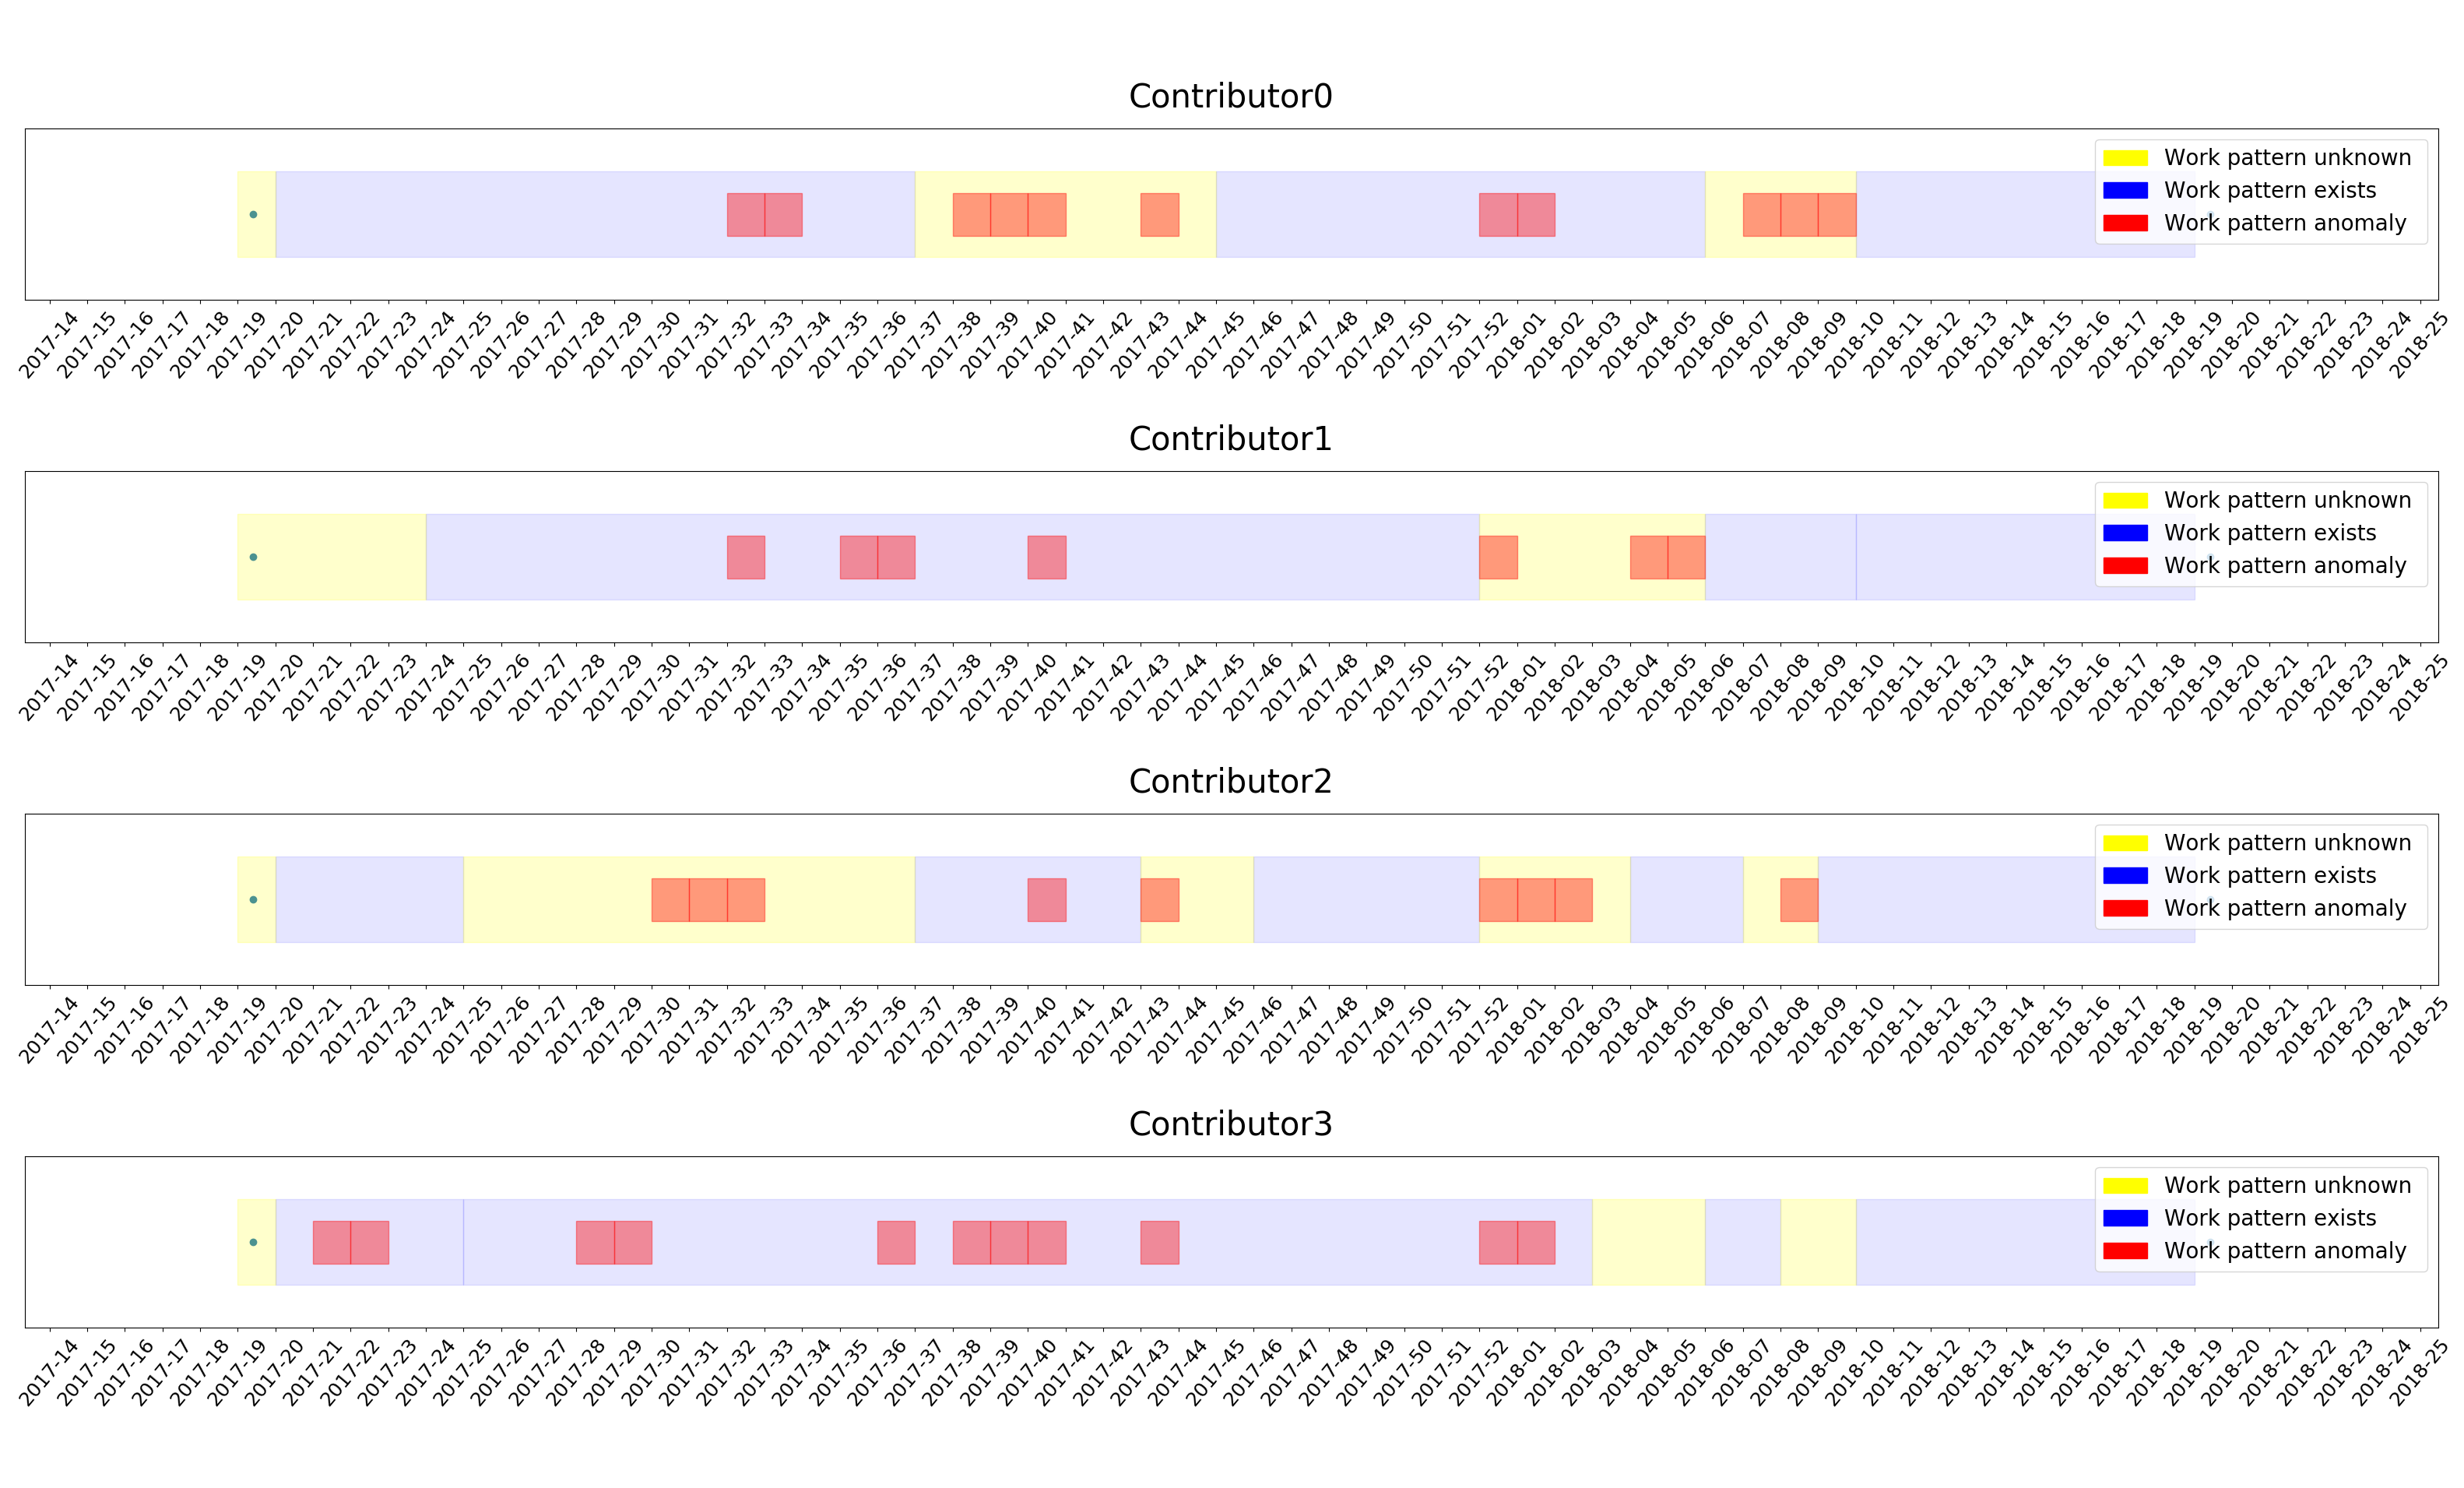
\includegraphics[scale=0.19]{./graphs/analysis/work-time-analysis-comparison}
    \centering
    \caption{The miss-out analysis graphs of the four employees from the survey.}\label{fig:miss-out-comparison}
\end{figure}

In Figure~\ref{fig:miss-out-comparison} the comparison between multiple employees can be seen.
\emph{Contributor0} and \emph{Contributor2} are working on flexible work time, which reflects in the inconsistencies in the work patterns (yellow sections in Figure~\ref{fig:miss-out-comparison}) of those contributors.
The other two contributors have very consistent working hours patterns, as can be seen by the long-lasting blue sections.


\section{Sleep Rhythm and Working Hours}

\subsection{Sleep Rythm}
To evaluate the significance of the punch card in terms of sleep rhythm analysis, a small survey in a closed community has been made.
A group of ten people, who know each other well, has been selected for this purpose.
Furthermore, a subset of four people has been chosen who were going to be evaluated.
The data gathered for the test group only contained their leisure time contributions, as their work repositories were not open-source.
All ten people then needed to assign the punch card of those four persons to a specific person.
The specific task given to test group was to assign each punch card to a specific person based on their knowledge about their sleep rhythm and leisure time behavior.

To this end, three quite similar patterns, from which one contributor has a very regular sleep rhythm (Subfigure 2 in Figure~\ref{fig:punchcard-survey}) and one pattern of a practically inexistent sleep rhythm (Subfigure 1 in Figure~\ref{fig:punchcard-survey}) have been selected.

For the three similar graphs, no significant results could be assessed, as the assignments were more or less random.
The contributor with the irregular sleep rhythm, on the other hand, got correctly assigned in all cases.

Sadly, as such a survey needs very specific targeting and a long lead time for data collection, it could only be executed on a small number of subjects.
Anyhow the result of this survey indicates that there exists a correlation between the structure of the punch card and the sleep and leisure time commit behavior of a contributor, even if it can only be accurately assigned in extreme cases.


\begin{figure}[H]
    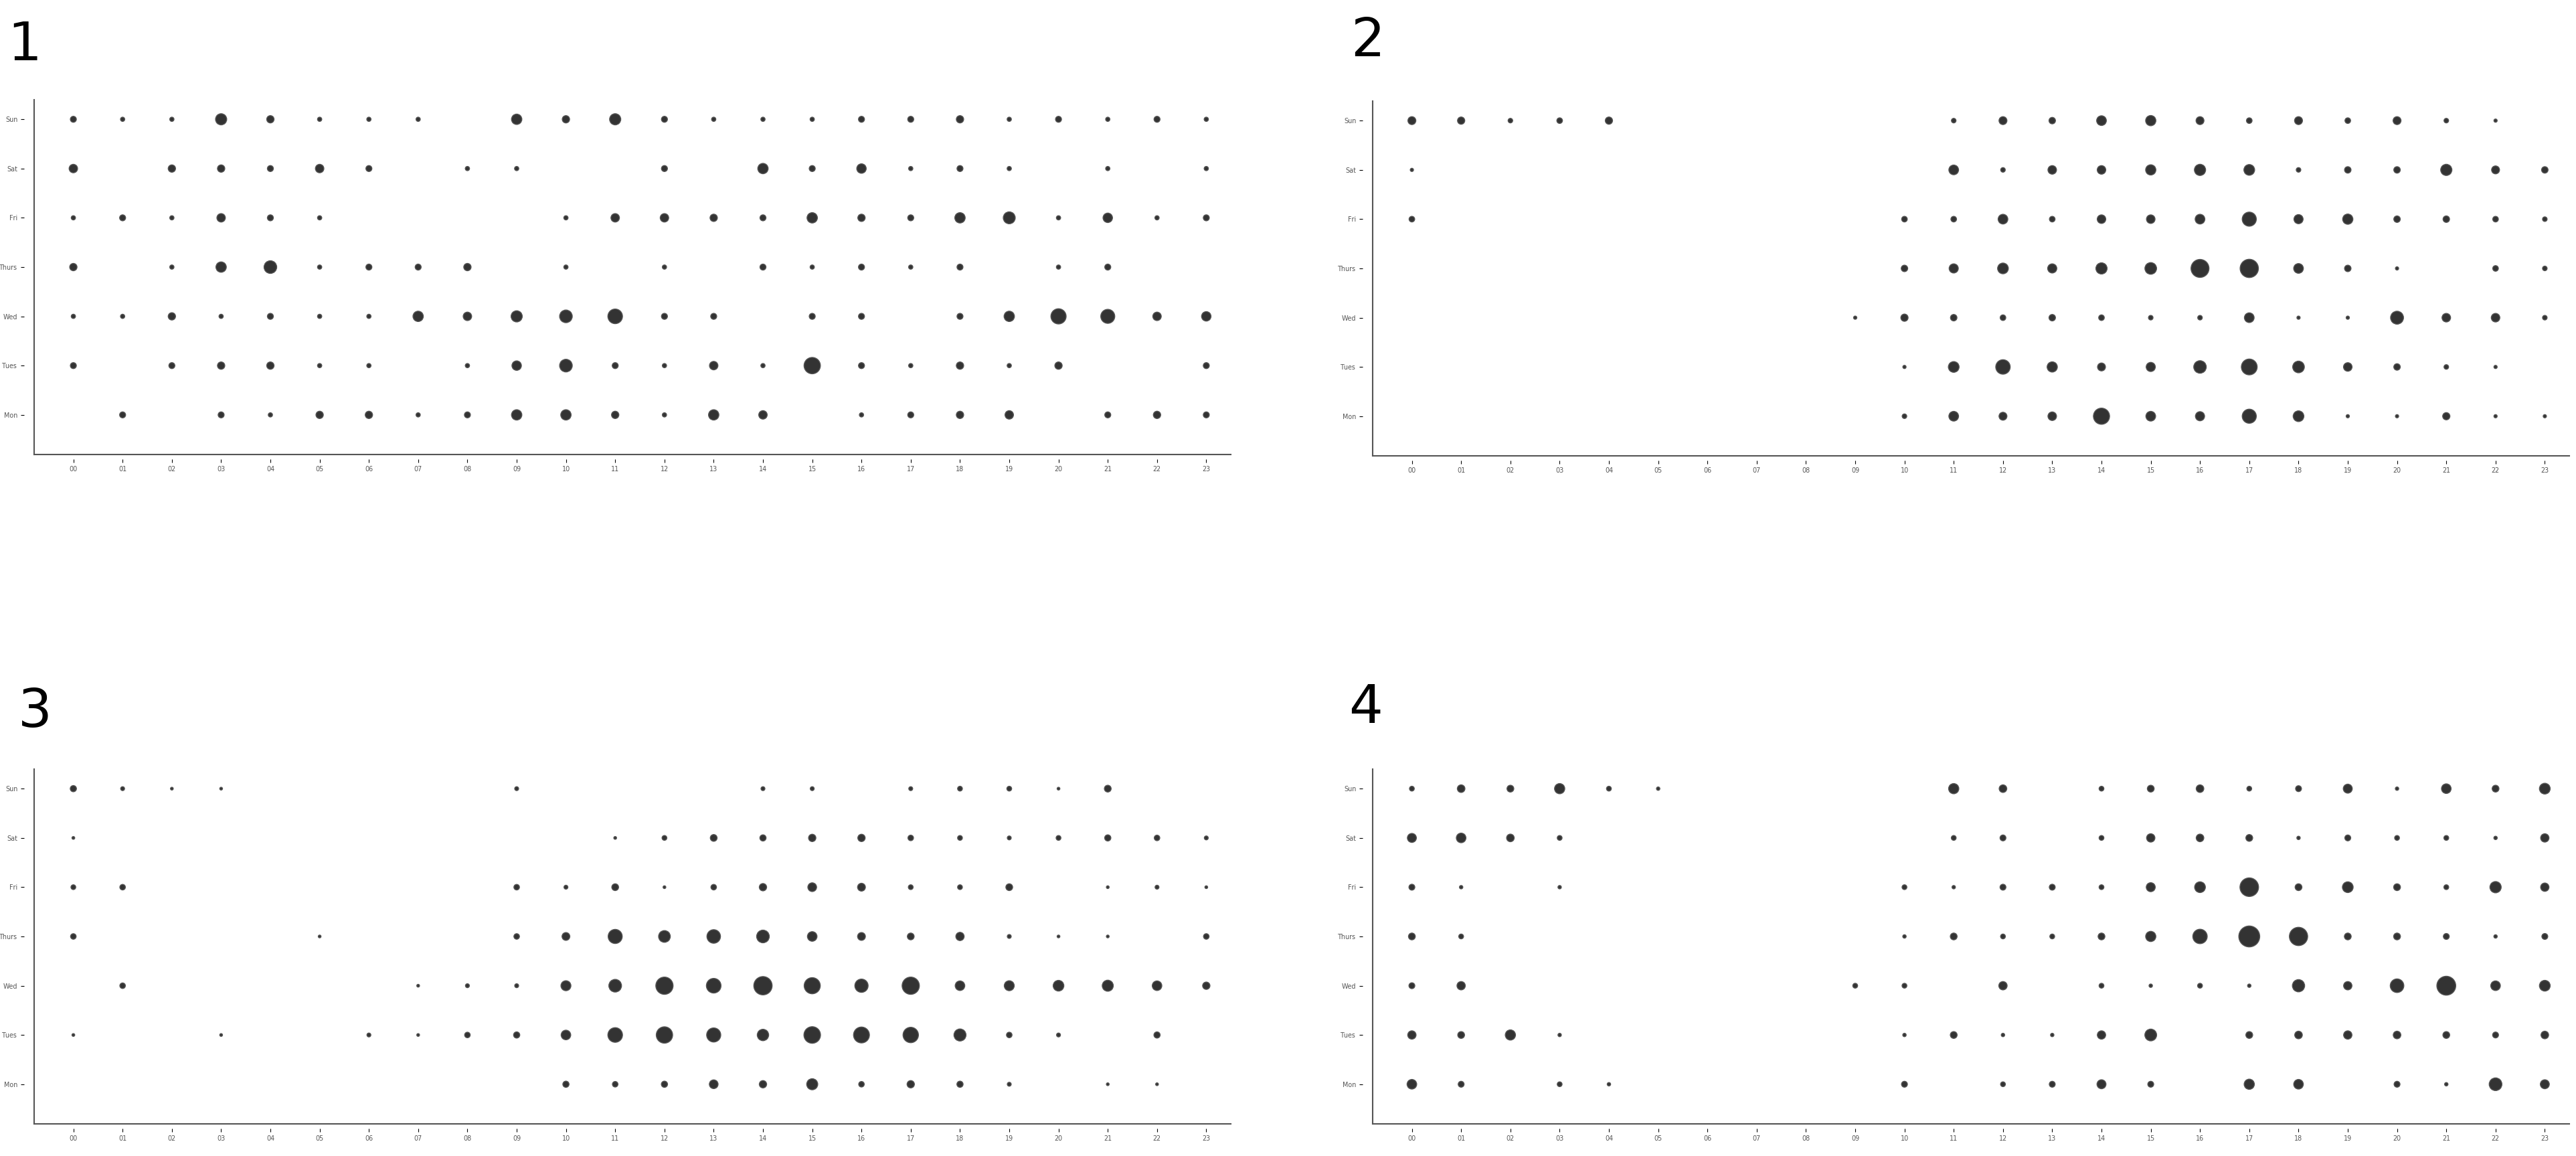
\includegraphics[scale=0.16]{./graphs/analysis/survey_combined}
    \centering
    \caption{The punch cards created and used for the test group in the survey.}\label{fig:punchcard-survey}
\end{figure}

\subsection{Employee or Open-Source Contributor}
To determine whether a punch card could be used to distinguish between an employee or an open-source volunteer, the results of the clustering described in Section~\ref{punchcard-implementation} have been utilized.
For this approach, two assumptions have been made.
A usual employee works between Monday and Friday during the day and only as an exception at the weekend, an example cluster can be seen in Figure~\ref{fig:normal-office-hours}.
An open-source volunteer works outside of the usual work shifts, which means early and late during weekdays and at the weekend, an example cluster can be seen in Figure~\ref{fig:leisure-time-hours}.

\begin{figure}[H]
    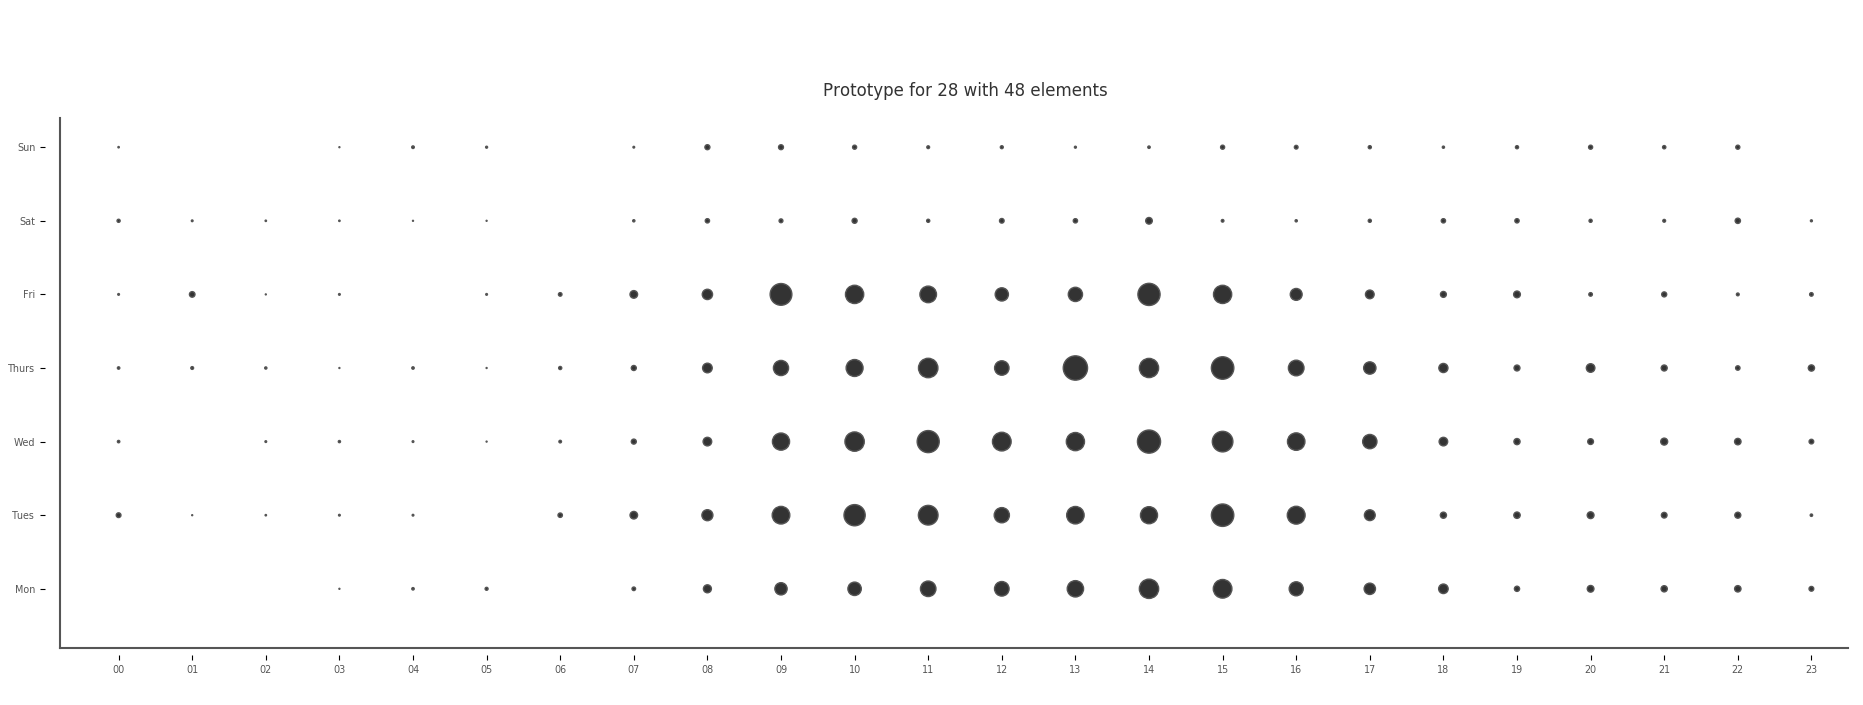
\includegraphics[scale=0.32]{./graphs/analysis-affinity/28}
    \centering
    \caption{Punch card of an example from an affinity propagation cluster of contributors with normal work shifts.
    A clear tendency to regular office working hours can be seen (Monday to Friday between 7:00 and 18:00 o'clock)}\label{fig:normal-office-hours}
\end{figure}

For each assumption, two representative clusters have been chosen and ten random persons have been selected from each cluster.
The manual verification is conducted by checking if the contributor mainly contributes to repositories which belong to the registered employee.
If no employee is registered, but other sources such as a homepage are provided, the information of these sources is checked for possible employee details as well.
In case no employee exists, it is examined whether the contributor pushes to their own and to open-source projects or rather to the repositories of a specific company.

\begin{figure}[H]
    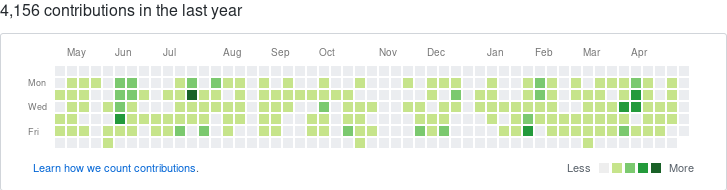
\includegraphics[scale=0.6]{./graphs/contribution-overview-alxhub}
    \centering
    \caption{Github contribution overview of a Google developer with the nickname alxhub.}\label{fig:github-contribution-overview}
\end{figure}

For this purpose, the Github contribution overview on the contributors' profile page has been used.
An example of such an overview can be seen in Figure~\ref{fig:github-contribution-overview}.
It provides a good overview of the usual weekday work pattern over the last year and allows to quickly inspect the repositories a contributor committed to at a specific month.

\begin{figure}[H]
    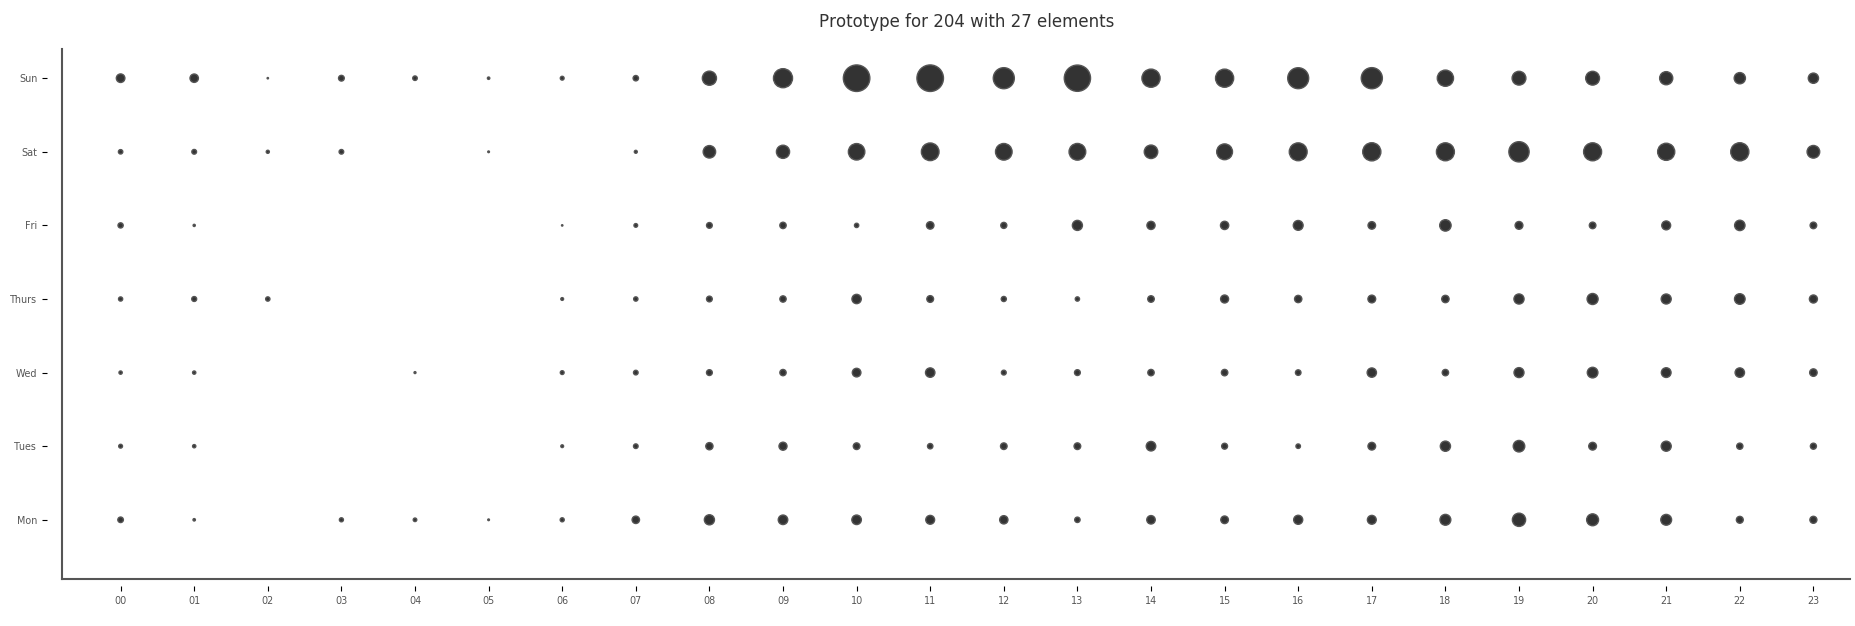
\includegraphics[scale=0.32]{./graphs/analysis-affinity/204}
    \centering
    \caption{Punch card of an example from an affinity propagation cluster of leisure time contributors. A clear tendency to contributions out of regular working hours and at the weekend.}\label{fig:leisure-time-hours}
\end{figure}

The representatives for the usual five-day week commit behavior were surprisingly accurate.
19 out of 20 considered contributors were mainly working on projects of their companies, with occasional commits to other open-source projects.
For the remaining contributor, it could not be determined if they work for a company.

The representatives for the leisure time commit behavior are mostly correct as well.
15 out of 20 considered contributors were irregularly contributing to either work unrelated open-source projects or to their own projects.
See Appendix~\ref{tbl:leasure-time-cluster-evaluation} for a table with the results of the leisure time cluster evaluation.
The remaining five contributors were either contributors working and committing to their employee's projects, but also to their own and open-source projects or employees with an untypical commit behavior.

This analysis shows quite well, that there is a correlation between the assumed patterns and the Github commit behavior or the usage of their Github accounts.
Unfortunately, the evaluation process for these results is very time consuming and thereby only a relatively small sample (n=40) has been chosen.
As it is not trivial to link the employee of a contributor to all their funded projects, all verification needed to be conducted manually.

\begin{landscape}
    \begin{table}[]
        \centering
        \captionof{table}{Employee cluster evaluation.}\label{tbl:employee-cluster-evaluation}
        \begin{tabular}{lllll}
            \toprule
            Nickname      & Employer     & Main projects                & Work related & Over 90\% work related \\
            \midrule
                          &              &                              &              &                        \\
            brettfo       & Microsoft    & visualfsharp                 & yes          & no                     \\
            aputinski     & Salesforce   & Salesforce                   & yes          & yes                    \\
            alxhub        & Google       & Angular                      & yes          & yes                    \\
            MatrixFrog    & Google       & Google Projects              & yes          & yes                    \\
            ryanemerson   & Red Hat      & Infinispan                   & yes          & no                     \\
            garagatyi     & Red Hat      & Eclipse and related projects & yes          & yes                    \\
            eternoendless & PrestaShop   & PrestaShop                   & yes          & yes                    \\
            initvector    & vanilla      & vanilla                      & yes          & yes                    \\
            kyhavlov      & HashiCorp    & HashiCorp                    & yes          & no                     \\
            XenoPhex      & CloudFoundry & CloudFoundry                 & yes          & yes                    \\
            gjoranv       & unknown      & vespa-engine/vespa           & probably     & yes                    \\
            doolse        & Equella      & Equella                      & yes          & yes                    \\
            leplatrem     & Mozilla      & Mozilla/Kinto                & yes          & yes                    \\
            StrongMonkey  & Rancher Labs & Rancher Labs                 & yes          & no                     \\
            lukaseder     & jOOQ         & jOOQ                         & yes          & yes                    \\
            DaazKu        & vanilla      & vanilla                      & yes          & yes                    \\
            brettcannon   & Microsoft    & Microsoft/Python             & yes          & yes                    \\
            isidorn       & Microsoft    & Microsoft Projects           & yes          & yes                    \\
            jackhorton    & Microsoft    & Microsoft Projects           & yes          & yes                    \\
            glasserc      & Mozilla      & Mozilla/Kinto                & yes          & yes                    \\
            nickwei84     & CloudFoundry & CloudFoundry                 & yes          & yes                    \\
            \bottomrule
        \end{tabular}
    \end{table}
\end{landscape}


\subsection{Bot Detection}
Another possible attack that opened up during the creation of the clusters was the detection of automatically committing programs, so-called \emph{bots}.
Several clusters showed a very consistent commit behavior around a specific hour, such a punch card can be seen in Figure~\ref{fig:bot-punchcard}.

\begin{figure}[H]
    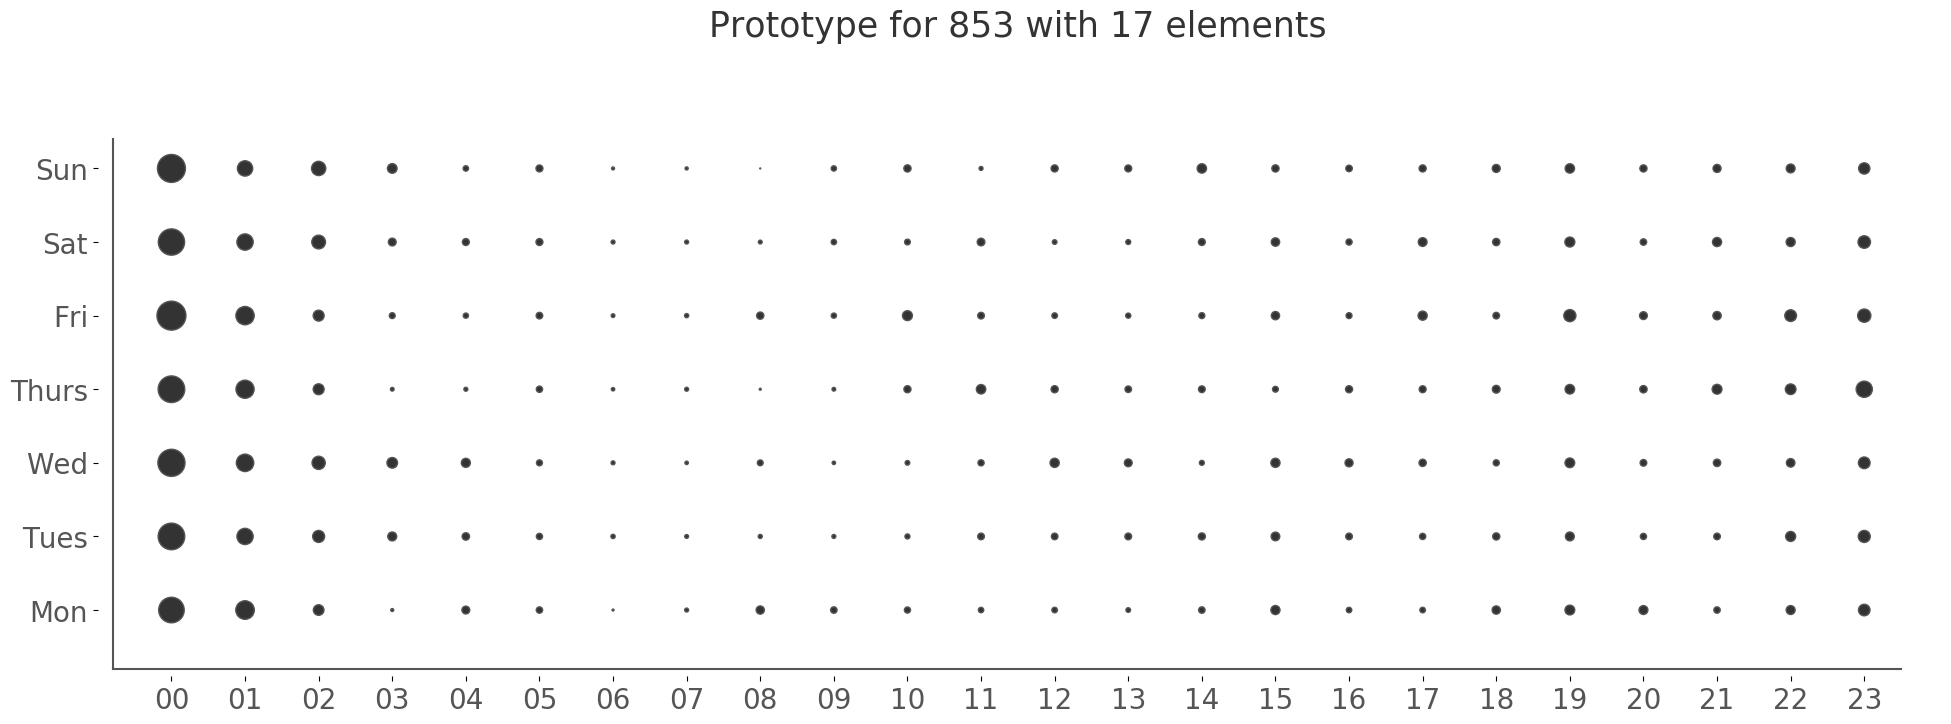
\includegraphics[scale=0.32]{./graphs/analysis/bot-punchcard}
    \centering
    \caption{A punch card with an extraordinary commit pattern around midnight. This might indicate a regularly automatically committing program, a so-called \emph{bot}}\label{fig:bot-punchcard}
\end{figure}

In the following, I implemented an algorithm which simply detected centroids with an extremely equally distributed pattern or patterns with a spike at a specific hour.
After a manual revision of the clusters detected by this methodology, it became apparent that only a very small subset of those clusters actually contained bots.
Even if the cluster contained bots there usually were only one or two of a much larger pool of cluster members.

Detection of bots in the outliers, which were not assigned to any cluster, did not seem to be promising as well.
Manual revision of over 100 possible candidates led to not a single bot.
After reviewing these results, I decided that there is currently no viable approach to this problem.


\subsection{Fingerprinting}
Another possible attack was to fingerprint a contributor and create a unique identifier by analyzing their commit behavior.

This attack soon proved to be unfeasible, as the pattern of a contributor can significantly differ from month to month, as can be seen in Figure~\ref{fig:october-punchcard} and Figure~\ref{fig:november-punchcard}.

\begin{figure}[H]
    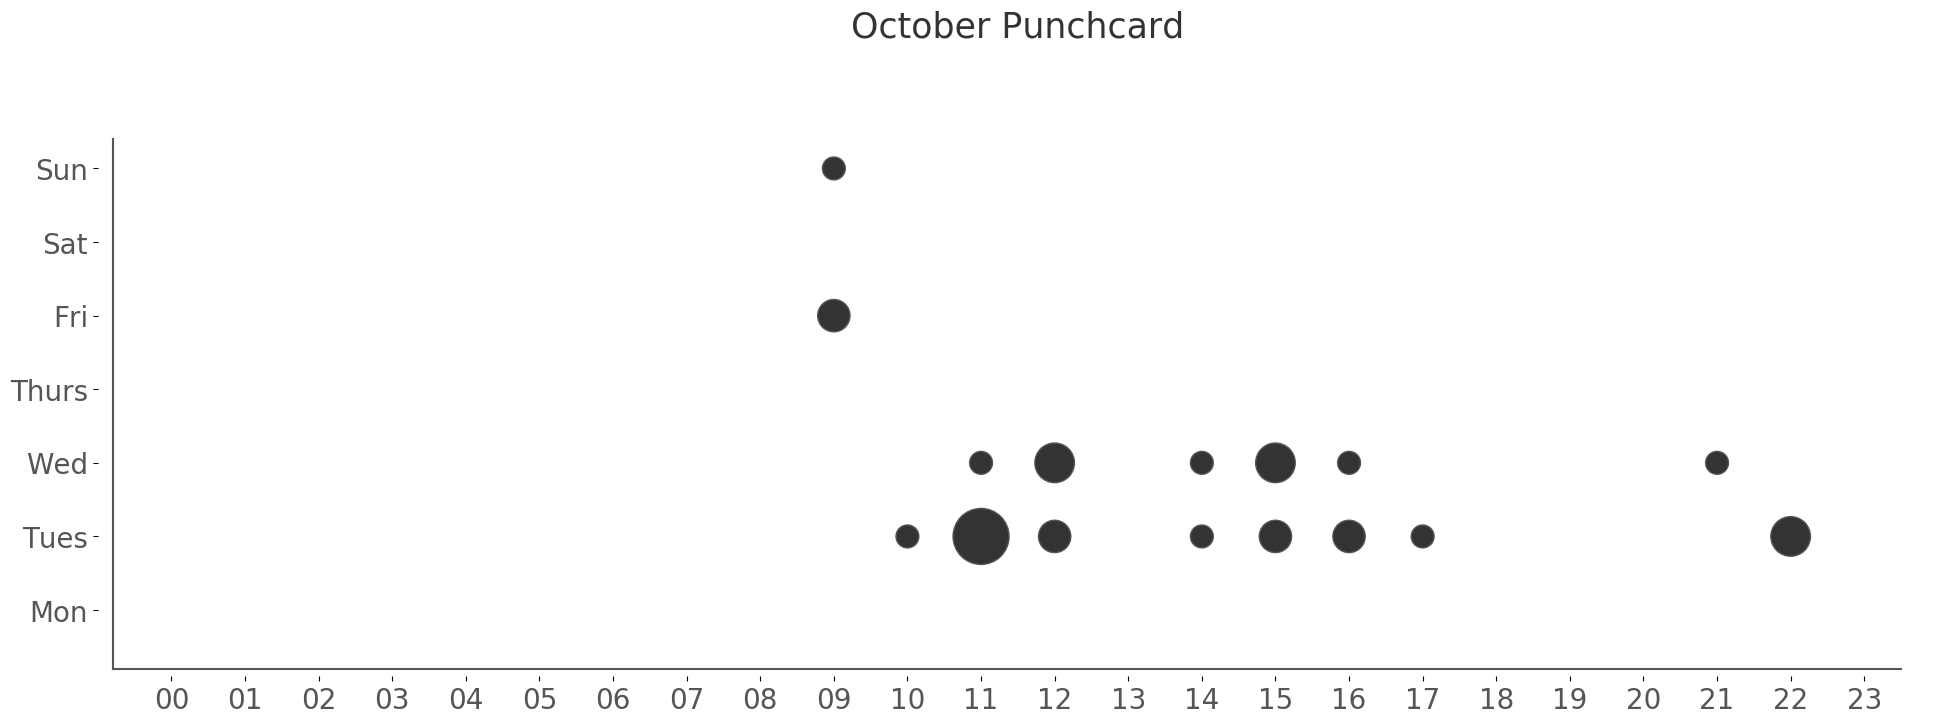
\includegraphics[scale=0.32]{./graphs/analysis/october-punchcard}
    \centering
    \caption{The author's punch card from October 2017.}\label{fig:october-punchcard}
\end{figure}

\begin{figure}[H]
    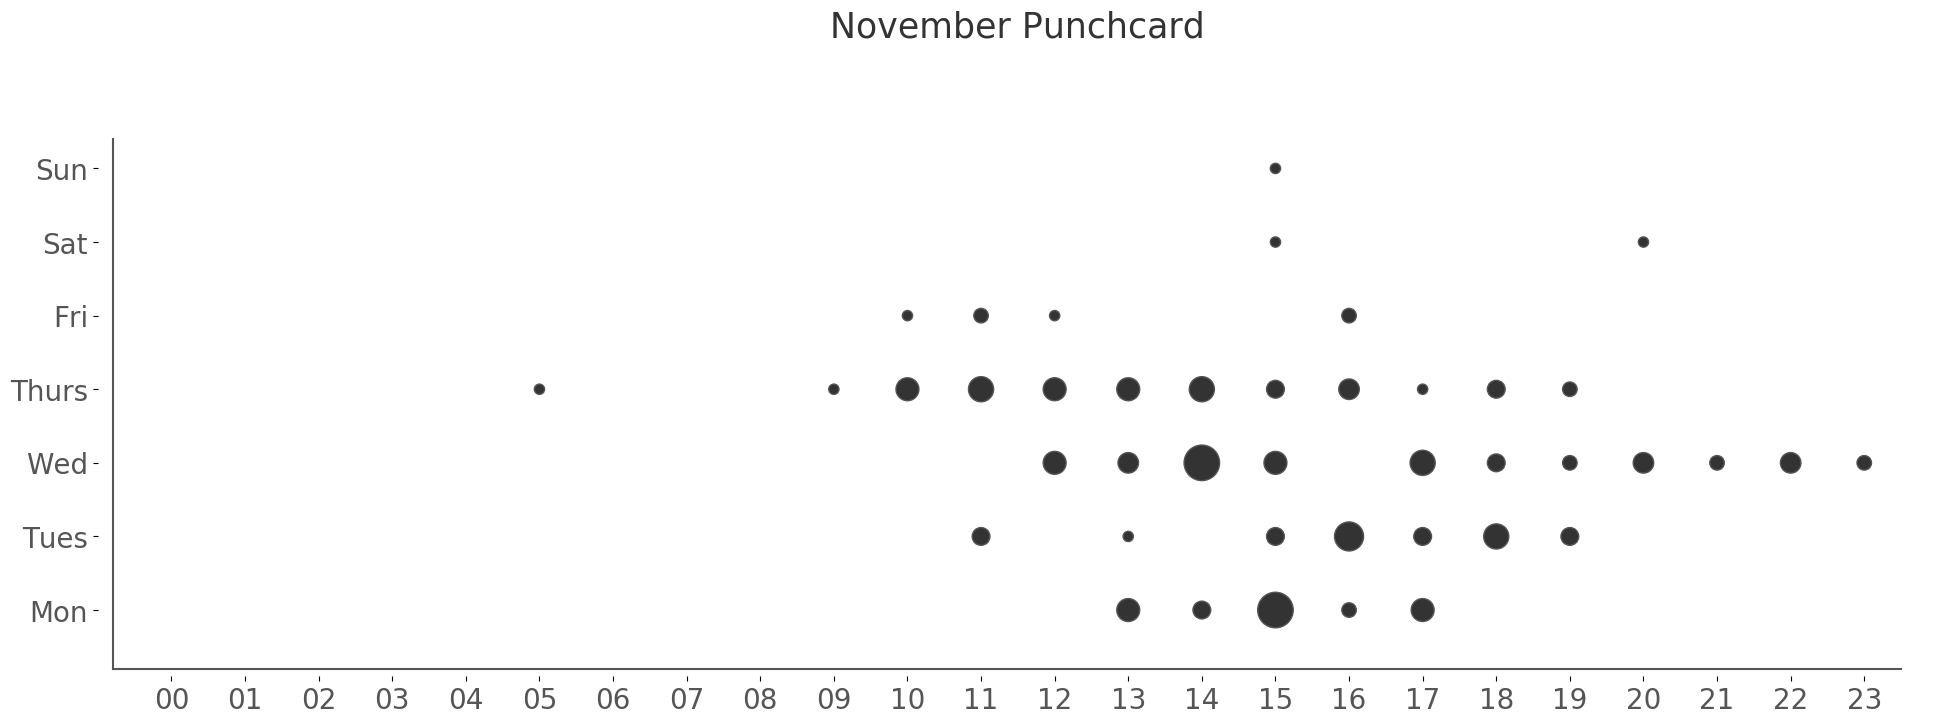
\includegraphics[scale=0.32]{./graphs/analysis/november-punchcard}
    \centering
    \caption{The author's punch card from November 2017.}\label{fig:november-punchcard}
\end{figure}

If the interval of a year is considered and the compared interval is shifted by a single month, the occurring changes are not that drastic, but still too different to see a consistent pattern over a longer time.
The commit behavior of people seems to be too inconsistent to create a unique fingerprint.


\section{Geographic Location}

First of all, it needs to be clarified that parts of this attack only works under specific circumstances.
Git commit timestamps are created by taking the current local time of the underlying \ac{os}.
If one wants to show the travel path of a target, the target's \ac{os} needs to automatically adjust the \ac{utc} offset accordingly to the current geographic location of the device.

This feature is available for newer versions of popular \acp{os}, such as \emph{Windows}~\footnote{Ivan Jenic, `Your Time Zone Can Now Switch Automatically in Windows 10', windowsreport.com, https://windowsreport.com/time-zone-automatic-switch-windows-10 (accessed, 24.04.2018)}
and \emph{Mac Os}, but they are not enabled by default.
It is also available for Linux, for instance, with the \emph{tzupdate} package~\footnote{`Set the system timezone based on IP geolocation', github.com, https://github.com/cdown/tzupdate (accessed, 24.04.2018)}, but it needs to be manually installed and activated.

\begin{figure}[H]
    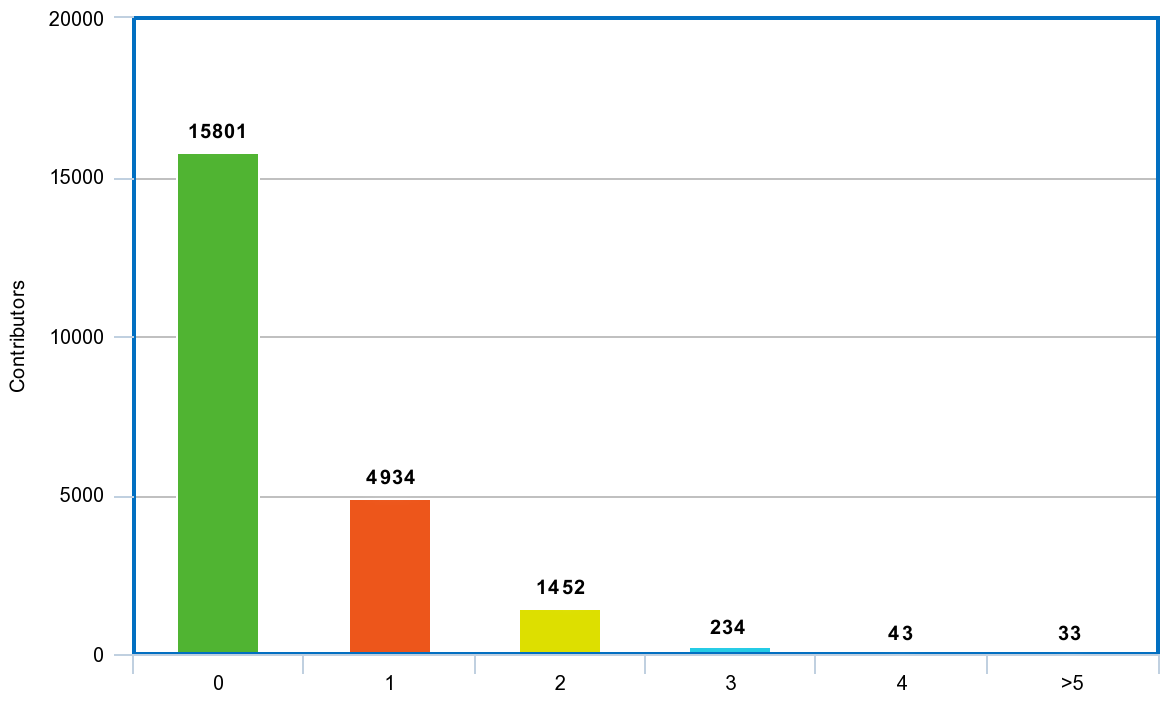
\includegraphics[scale=0.38]{./graphs/analysis/timezone-switch-distribution}
    \centering
    \caption{Distribution of users according to the amount of timezone switches detected by the algorithm.
    The major part of all contributors does not have any detectable timezone changes.}\label{fig:timezone-switch-distribution}
\end{figure}

Figure~\ref{fig:timezone-switch-distribution} shows the number of contributors in relation to the number of detected timezone switches.
On about 70\% of considered contributors, only a single timezone has been detected, looking at the last year.
These 70\% do either not commit when they travel, their \acp{os} do not synchronize the timezone accordingly to their location or they simply did not travel in the last two years.

\begin{figure}[h]
    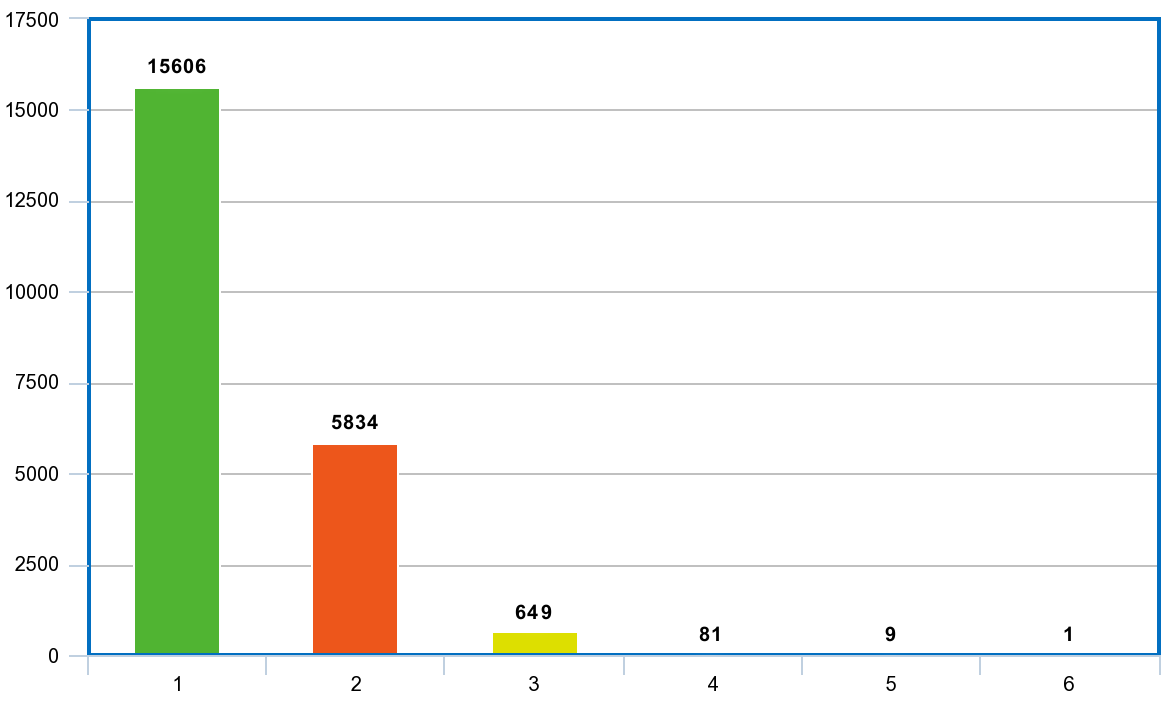
\includegraphics[scale=0.38]{./graphs/analysis/timezone-distribution}
    \centering
    \caption{Distribution of users according to the amount of the different timezones detected by the algorithm.}\label{fig:timezone-distribution}
\end{figure}

In Figure~\ref{fig:author-home-location} the visualized home location analysis of the author can be seen.
Regions marked in dark green are regions in which the contributor is likely to live.
The light green region represents the timezone of the home location.
As you can see in Figure~\ref{fig:author-home-location} the country of French Guiana is also marked as a possible home location.
This problem occurs due to the several conversions between country names and codes, which were necessary as stated in Section~\ref{timezone-implementation}.
This misassignment only happens during the visualization process of the results and thereby does not affect the results of the analysis.

\begin{figure}[h]
    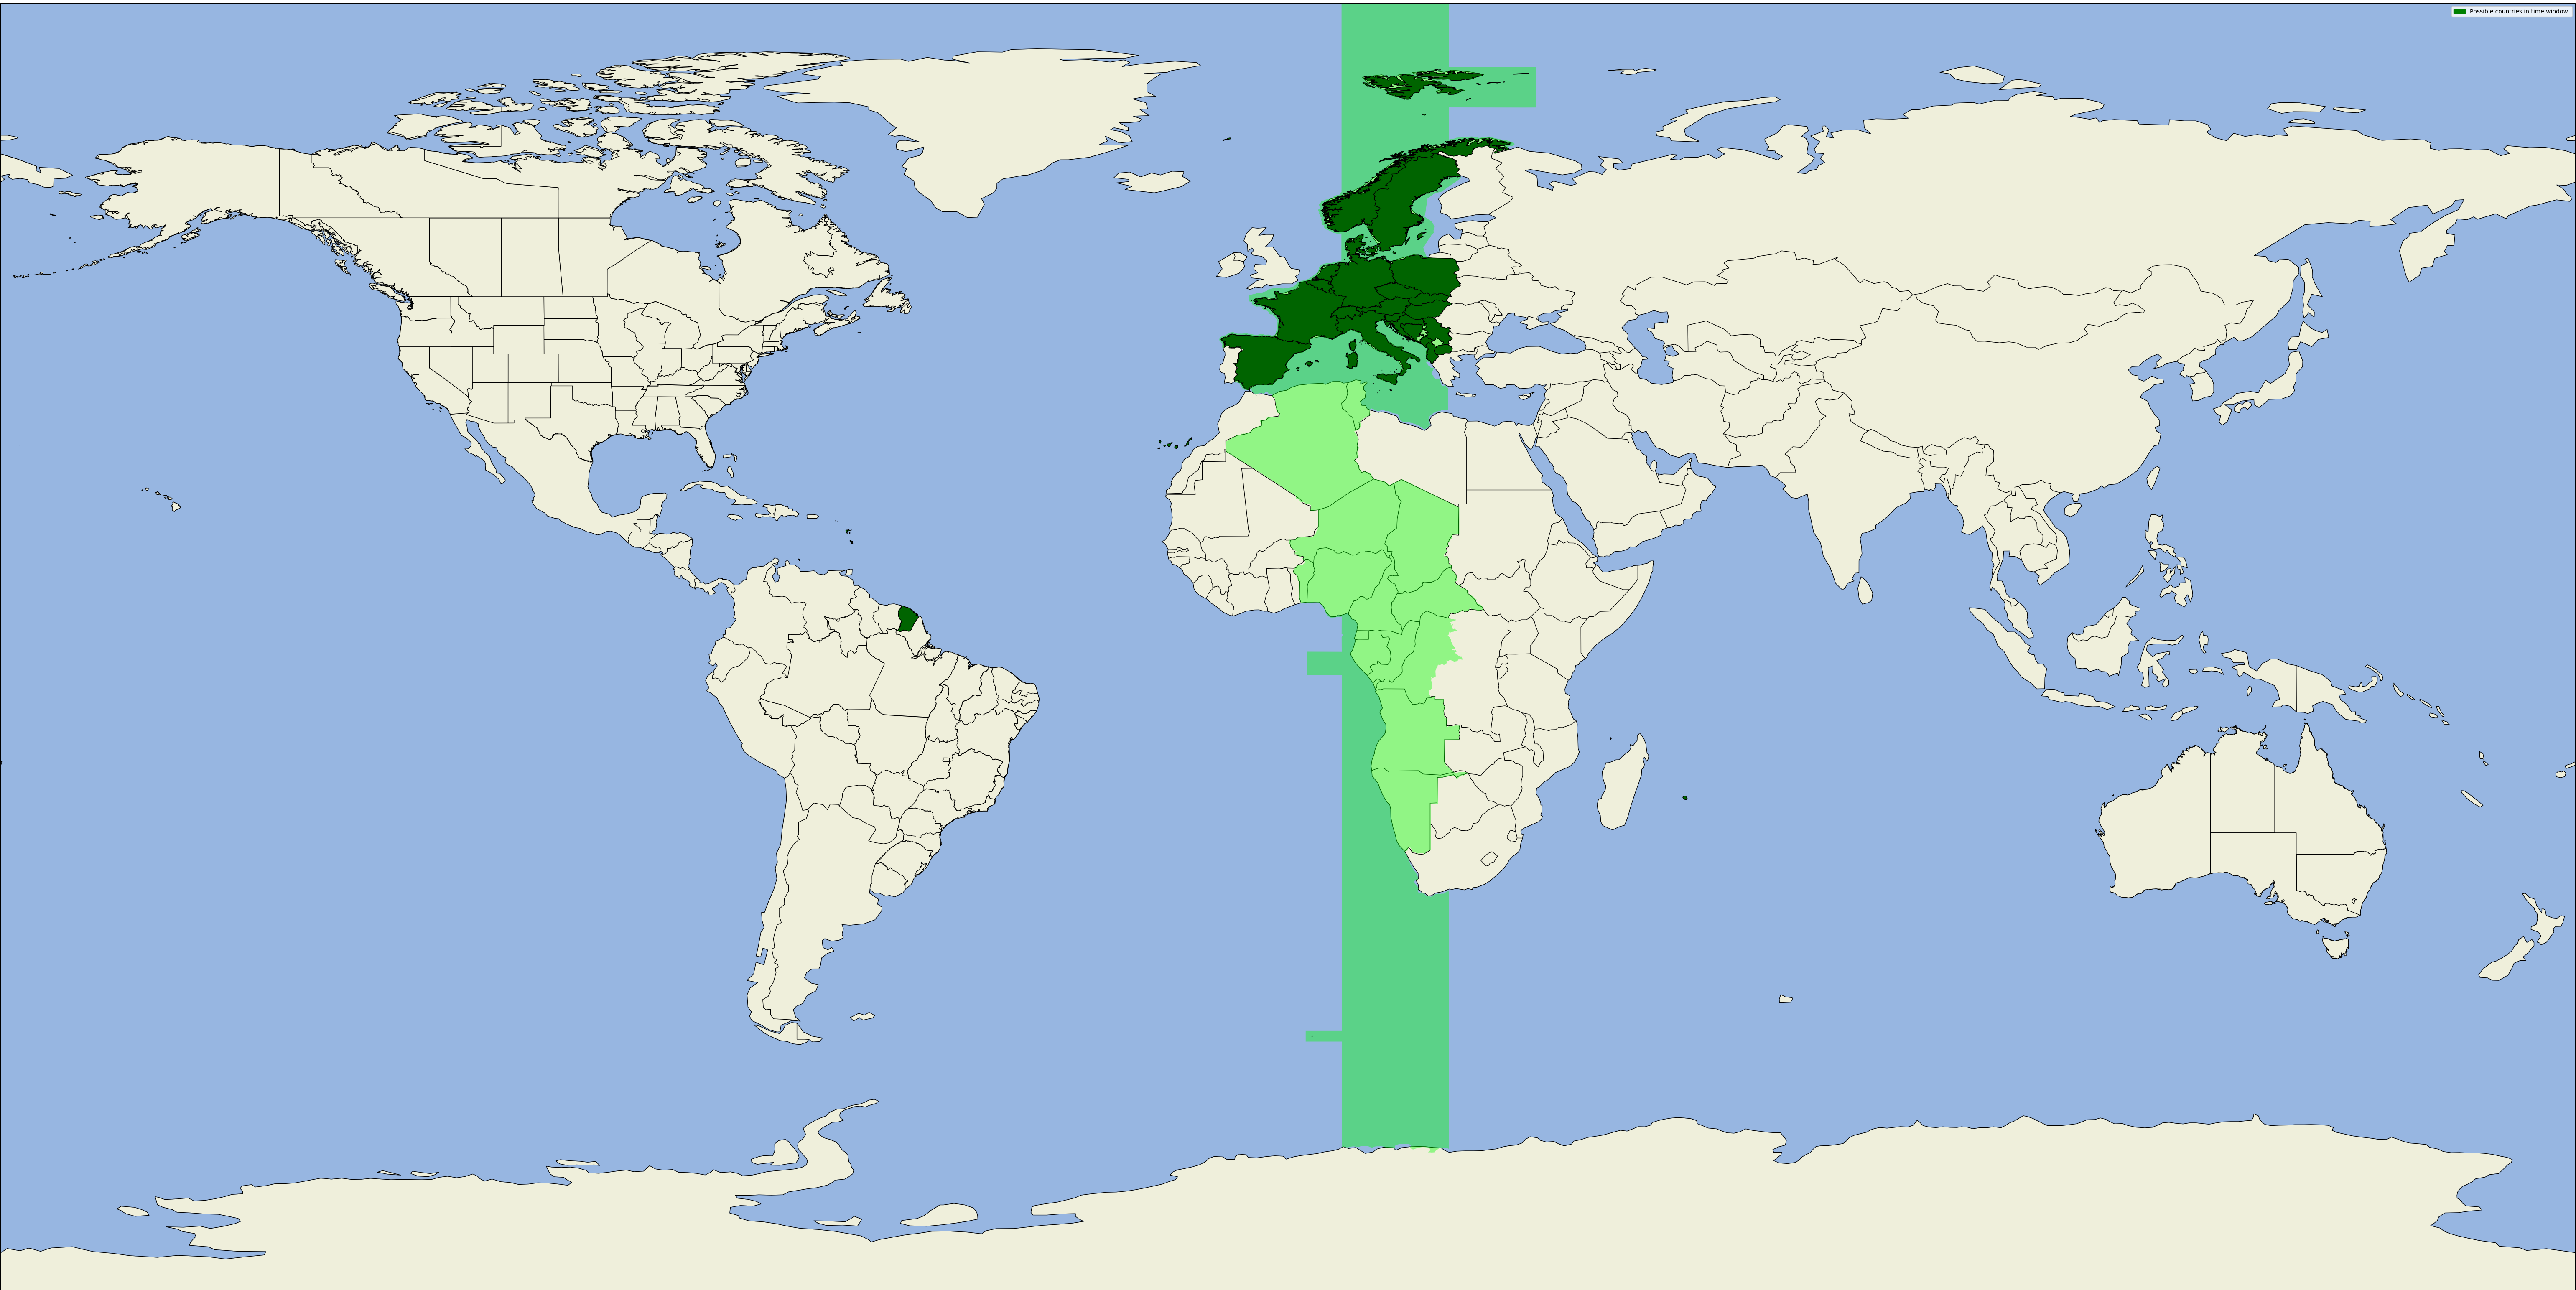
\includegraphics[scale=0.10]{./graphs/analysis/author-home-location}
    \centering
    \caption{The visualized home location analysis of the author.
    The light green indicates the timezone the target is probably in.
    The dark green color shows the remaining countries after considering \ac{dst} switches.}\label{fig:author-home-location}
\end{figure}

To evaluate the overall precision of the geographic location results, the correctness of the determined home locations are checked.
Github allows users to specify a string for their current home location, which is also collected during the data aggregation process.
Unfortunately, there are no conventions on how this string has to look like.
Initially, I tried to pass these strings to the OpenStreetMap \ac{api}, but this resulted in too many wrongly assigned locations.
The data provided by the users was obviously too arbitrary and full of mistakes for OpenStreetMap to handle.

As a result, I decided to manually choose a subset of locations by looking for distinct identifiers in the location strings.
For instance, every home location of a contributor, that contained \emph{Germany} or \emph{Deutschland} in their location string, should be in the timezone \inlinecode{Europe/Berlin}, which switches between \ac{cet} and \ac{cest}.
I created 14 such rules and was thus able to validate the home location of about 4200 contributors.
The assignment of the contributors home location was correct in about 82\% of the considered contributors.

It needs to be noted, that the accuracy of this result is quite certainly deteriorated by location strings which contain ambiguous information.
On manual review of the location strings there were strings such as \inlinecode{I love NYC} which belongs to a developer living in Germany.
The result might also be deteriorated by contributors who moved to another country in the last year, as we cannot detect those for sure.

It also needs to be noted, that the \ac{iana} database does not always have exact mappings for countries to their timezone.
For many countries or states, the current or an old capital city is used.
Some countries do not have an own timezone, such as Japan, which is included in \inlinecode{Pacific/Palau}.
The \ac{iana} database is the currently best viable approach, but for better results and a more fine-grained resolution, a specific mapping between countries, states and time zones would be necessary.

Nevertheless, an accuracy of 76\% clearly shows, that it is possible to narrow down the location of a contributor to a timezone and even to a subset of countries, see Table~\ref{home-location-table} for reference, by simply looking at their git commit timestamps.

\begin{landscape}
    \begin{table}[h]
        \centering
        \begin{tabular}{llrrrr}
            \toprule
            Query string & Expected timezone string & Considered & Correct & Timezone strings after DST & Before DST  \\
            \midrule
            & & & & & \\
            San Francisco        & US/Pacific           & 772        & 639     & 12.07   &  18     \\
            NYC, NY, New York    & America/New\_York    & 485        & 366     & 23.60   &  52     \\
            India                & Asia/Colombo         & 148        & 127     & 4       &  4      \\
            UK, United Kingdom   & Europe/London        & 667        & 510     & 13.14   &  22     \\
            France               & Europe/Paris         & 490        & 421     & 31.59   &  40     \\
            New Zealand          & Pacific/Auckland     & 59         & 52      & 4.76    &  9      \\
            Germany, Deutschland & Europe/Berlin        & 976        & 846     & 31.48   &  38     \\
            Poland               & Europe/Warsaw        & 180        & 154     & 31.56   &  40     \\
            Italy                & Europe/Rome          & 130        & 112     & 31.39   &  41     \\
            Tokyo                & Pacific/Palau        & 61         & 48      & 8.51    &  12     \\
            Spain                & Europe/Madrid        & 129        & 116     & 32.83   &  40     \\
            Los Angeles          & America/Los\_Angeles & 86         & 76      & 12.24   &  18     \\
            Adelaide             & Australia/Adelaide   & 2          & 2       & 4.00    &  4      \\
            Mexico               & Mexico/General       & 13         & 7       & 11.62   &  39     \\
            \bottomrule
        \end{tabular}
        \caption{Results of the home location evaluation.
        The first column shows the comma separated strings by which contributors are selected depending on their location.
        The second column is the timezone that is expected to be in the remaining home location timezone string set.
        }\label{home-location-table}
    \end{table}
\end{landscape}


\chapter{Conclusion and Outlook}

The study set out to determine how feasible and precise data mining attacks on simple Git metadata could be.
All three performed attacks, lead to promising results and showed potential for malicious usage.

The miss-out analysis showed that it is possible to automatically detect holiday and sick-leave anomalies.
Additionally, it is capable of detecting other anomalies in the developer's work pattern.

Analyzing the Git commit timestamps to narrow down the geographic location of a user-led to a significant reduction of possible locations on the globe.
With a proper test group, it is also likely to prove, that the other detected timezones represent the travel history of the target.

The analysis of punch cards showed, that it is possible to detect developers working at regular five day office hours and to distinguish between working employees and leisure time developers.

However, it must be noted that in all attacks only a small amount of the available data was used.
Simply using the Git commit timestamps allowed us to perform analyses such as narrowing down the location of a contributor.
The possible applications for the remaining data, like actual changes in code, references of contributors between repositories or commit messages, are extensive.

If one would add additional data from Github, such as followers, stars or information from their issues system, the results could become even more accurate.
Developers around the world provide metadata about themselves on a daily basis, probably without knowing how much they are actually exposing.
To prevent the unauthorized usage and abuse of this data, we need to create countermeasures or prevent exposing this data in the first place.

Luckily the \ac{eu} set an example by enforcing the \ac{gdpr}, which is a regulation that strictly rules the handling of any user data.
But there are still many countries left in the world, that do not have such strict rules and that might need ways to protect their privacy from being invaded.

While \emph{Gitalizer} is a foundation for data aggregation and the conduct of rather simple analyses, there is a necessity for more detailed research with better sources for ground truth.
Additionally, more statistics about the mining process would be convenient for evaluating the research results, such as the ratio between starred and contributed repositories.
\emph{Gitalizer} is a quite complex program, but it is well documented and should allow other people to easily jump into using it.

Many of the attacks mentioned in Section~\ref{attack-goals} are not implemented, as they did not fit in the scope of this thesis.
Implementing those could be the topic of another bachelor thesis or for a subsequent master thesis.

Furthermore, it would be interesting to explore the possibilities of countermeasures such as obfuscating Git commit timestamps.


\begin{appendices}
\chapter{Leisure time cluster evaluation}
\begin{landscape}
    \begin{table}[]
        \centering
        \captionof{table}{Leisure time developer cluster evaluation.}\label{tbl:leasure-time-cluster-evaluation}
        \begin{tabular}{llllll}
            \toprule
            Nickname      & Employer      & Main projects exists               & Work related    & Over 90\% work related & Commits rarely \\
            \midrule
                          &               &                                    &                 &                        &                \\
            craigbarratt  & unknown       & backuppc                           & unknown         & unknown                & yes            \\
            hackebrot     & Mozilla       & Own repos, open-source             & no              & no                     & no             \\
            itamarnet     & unknown       & Open-source                        & no              & no                     & yes            \\
            JamesNK       & unknown       & Own repos                          & no              & no                     & no             \\
            kpreid        & unknown       & Own repos                          & no              & no                     & yes            \\
            vrasneur      & unknown       & Own repos                          & no              & no                     & yes            \\
            chrissimpkins & SourceFoundry & Own repos, SourceFoundry           & yes             & no                     & no             \\
            klauscfhq     & Cookfood HQ   & Own repos                          & no              & no                     & no             \\
            knowthelist   & unknown       & Own repos                          & no              & no                     & yes            \\
            larskanis     & Comcard       & Open-source                        & no              & no                     & no             \\
            NickeManarin  & unknown       & Own repos                          & no              & no                     & yes            \\
            obilodeau     & GoSecure      & GoSecure                           & yes             & no                     & no             \\
            piotrmurach   & unknown       & Own repos                          & no              & no                     & no             \\
            hauke         & unknown       & Open-source                        & unknown         & unknown                & yes            \\
            rspeele       & unknown       & Own repos                          & no              & no                     & yes            \\
            DylanC        & PhotoFlare    & PhotoFlare                         & yes             & yes                    & yes            \\
            Gitmaninc     & unknown       & SecWiki                            & no              & no                     & yes            \\
            lgreski       & unknown       & Own repos                          & no              & no                     & yes            \\
            vitaut        & Facebook      & Open-source                        & no              & no                     & no             \\
            wikimatze     & MyHammer AG   & Own repos, open-source             & no              & no                     & yes            \\
            schaal        & unknown       & Own repos                          & no              & no                     & yes            \\
            \bottomrule
        \end{tabular}
    \end{table}
\end{landscape}

\end{appendices}


\begingroup
    \footnotesize
    \listoffigures
    \let\clearpage\relax
    \listoflistings{}
    \listoftables
\endgroup

\renewcommand*{\bibfont}{\footnotesize}
\printbibliography{}

\chapter*{Eidesstattliche Erklärung}
\onehalfspace{}
„Hiermit versichere ich an Eides statt, dass ich die vorliegende Arbeit im
Studiengang Informatik selbstständig verfasst und keine anderen als die
angegebenen Hilfsmittel – insbesondere keine im Quellenverzeichnis nicht
benannten Internet-Quellen – benutzt habe. Alle Stellen, die wörtlich oder
sinngemäß aus Veröffentlichungen entnommen wurden, sind als solche kenntlich
gemacht. Ich versichere weiterhin, dass ich die Arbeit vorher nicht in einem
anderen Prüfungsverfahren eingereicht habe und die eingereichte schriftliche
Fassung der auf dem elektronischen Speichermedium entspricht.“
\singlespace{}

\vspace{1cm}

\begin{tabular}{ll}
    \centering
    \makebox[5cm]{\hrulefill} & \makebox[5cm]{\hrulefill}\\
    Ort, Datum & Unterschrift \\
\end{tabular}


\end{document}
